\documentclass{article}

%%%%%%%%%%%%%%%%%%%%%%%%%%%%%%%%%%%%%%%%

\usepackage[utf8]{inputenc}

%%%%%%%%%%%%%%%%%%%%%%%%%%%%%%%%%%%%%%%%

\usepackage{tikz}
\usepackage{pgfplots}
\pgfplotsset{compat=1.5}

\usetikzlibrary{external}
\tikzexternalize
\tikzsetexternalprefix{tikzexternal/}

%%%%%%%%%%%%%%%%%%%%%%%%%%%%%%%%%%%%%%%%

\usepackage{amsmath,amsfonts,amssymb}
\renewcommand{\baselinestretch}{1.0}
\usepackage{graphicx}
\usepackage[colorlinks=true, allcolors=blue]{hyperref}
\definecolor{gray}{gray}{0.75}
\definecolor{ligray}{gray}{0.9}
\usepackage{lscape}
\usepackage{enumitem}

\usepackage{chngcntr}
\counterwithin{figure}{section}
\counterwithin{table}{section}

%%%%%%%%%%%%%%%%%%%%%%%%%%%%%%%%%%%%%%%%

\setlength{\parindent}{0pt}
\setlength{\parskip}{\medskipamount}
\usepackage{setspace}

%%%%%%%%%%%%%%%%%%%%%%%%%%%%%%%%%%%%%%%%

\usepackage{newtxtext,newtxmath}

% Instead of the above, use this for arXiv:

%\usepackage{txfonts}
%\usepackage{textcomp}
%\usepackage{eurosym}
%\let\texteuro\euro

%%%%%%%%%%%%%%%%%%%%%%%%%%%%%%%%%%%%%%%%

\newcommand{\unit}[1]{\ensuremath{\mathrm{#1}}}
\newcommand{\micron}{\mbox{$\mu$m}}
\newcommand{\mm}{\mbox{mm}}
\newcommand{\sqmm}{\mbox{mm$^2$}}
\renewcommand{\deg}{\mbox{deg}}
\newcommand{\sqdeg}{\mbox{$\deg^2$}}
\newcommand{\persqdeg}{\mbox{$\deg^{-2}$}}
\newcommand{\arcmin}{\mbox{arcmin}}
\newcommand{\sqarcmin}{\mbox{\arcmin$^2$}}
\newcommand{\persqarcmin}{\mbox{\arcmin$^{-2}$}}
\newcommand{\arcsec}{\mbox{arcsec}}
\newcommand{\sqarcsec}{\mbox{\arcsec$^2$}}
\newcommand{\persqarcsec}{\mbox{\arcsec$^{-2}$}}
\newcommand{\Hs}{\mbox{$H_\mathrm{s}$}}
\newcommand{\CaF}{\ensuremath{\mathrm{CaF_2}}}

\newcommand{\TODO}[1]{\textcolor{red}{TODO: #1}}

%%%%%%%%%%%%%%%%%%%%%%%%%%%%%%%%%%%%%%%%

\begin{document}

\pagestyle{empty}

\begin{center}
\Large \bfseries
DDRAGO Interim Instrument\\Mechanical Design
\end{center}

\vspace{2cm}

\begin{center}

\begin{center}
\begin{tabular}{ll}
Prepared by:&Rosalía Langarica\\
&Alejandro Farah\\
&Salvador Cuevas\\
&Alan M. Watson\\
Approved by:&Alan M. Watson\\
Reference&GFT-MD-A3135-041-UNAM\\
Version:&3.0\\
Date:&9 May 2018\\
\end{tabular}
\end{center}

\vspace{\fill}

%\begin{center}
DDRAGO Project\\
Instituto de Astronomí­a\\
Universidad Nacional Autónoma de México
\end{center}

\clearpage
\section*{Document Change Record}

\begin{itemize}

\item Version 3.0 of 9 May 2018.

Designed the DDRAGO interim instrument and removed all material about the DDRAGO definitive instrument and CAGIRE.

\item Version 2.0 of 15 September 2017.

{\it Modifications from the previous version}

\begin{itemize}
\item Updated the design and analysis of the support structure.
\item Removed passive ventilation of the support structure.
\item Updated the designs of the lens mounts to use silicone O-rings for thermal compensation.
\item We will use a primer with the Krylon 1602 paint.
\end{itemize}

\item Version 1.0 of 22 January 2017.

Initial version.
\end{itemize}

\clearpage

\section*{Applicable Documents}

\begin{enumerate}[label={AD\arabic*}]
\item \label{management-plan} Watson, A.~M., “DDRAGO Interim Instrument Management Plan”, GFT-PL-A3135-045-UNAM, version 2.0.
\item \label{FPRD} Vives, S., R\'egal, X., \& Floriot, J., “Functional and Performance Requirements Documents”, version 3.3.
\item \label{telescope-icd} Floriot, J., \& Vola, P., “Telescope – Instrument
Interface Control Document”
\item \label{product-tree} Watson, A. M., “DDRAGO Product Tree”
\item \label{optics} Fuentes-Fernández,~J., Watson, A. M., \& Cuevas, S., “COLIBRÍ Optical Design”, GFT-OD-A3135-040-UNAM-3.0
\item \label{aiv} Cuevas,~S., Fuentes-Fernández,~J., Watson,~A.~M., \& Ángeles,~F., “DDRAGO Interim Instrument AIV Plan”, GFT-OD-A3135-043-UNAM-2.0
\item \label{control} Watson,~A.~M., \& Ángeles,~F., “DDRAGO Interim Instrument
Control System Design”, GFT-ED-A3135-042-UNAM-2.0

\end{enumerate}

\section*{Reference Documents}

\begin{enumerate}[label={RD\arabic*}]
\item \label{yoder15} Yoder, P. R and Vukobratovich, D., ``Opto-mechanical Systems Design", CRC Press, Fourth Ed., Vol. 1, Section 11.4.3. (2015)

\item \label{karow} Karow, H.H., [Fabrication methods for Precision Optics], Wiley, New York (1993).

\item \label{hopkins} Hopkins, R.E., “Lens Mounting and Centering”, chap. 2, [Applied Optics and Optical Engineering], Vol. VIII, Academic Press, New York (1980).
\item \label{ino} http://www.ino.ca/en/examples/lens-auto-centering-technology/

\item \label{parker} Parker O-Ring Handbook. 2001 Edition. Catalog 5700A/US, Section II, p.27.
Parker Hannifin Corporation, Cleveland, OH.

\item \label{black} Robinson,~F.~D., “RATIR Black Paint”, unpublished technical report, 2010.

\end{enumerate}

\clearpage

\pagestyle{plain}

\tableofcontents
\clearpage

\listoffigures
\clearpage

\listoftables
\clearpage

\section{Introduction}

This document describes the mechanical design of the DDRAGO interim instrument. This is a single-channel optical imager with a $4\mathrm{k}\times4\mathrm{k}$ CCD with a field of 26 arcmin square and five filters. 

The interim instrument is essentially an unfolding of the blue channel of the DDRAGO definitive instrument. The definitive instrument has a doublet (L1+L2) followed by reflections off two dichroics (D1 and D2), followed by another lens (L3), a filter wheel (BFW), and a CCD detector (BDET). The interim instrument removes the reflections off the two dichroics, but keeps the other optical components.

The full motivation of the interim imager is described in \ref{management-plan}. Here, we will simply repeat that the interim instrument is intended to provide a full-field instrument for optical tests of the telescope at the Observatoire de Haute-Provence (OHP) in 2019. However, it could also serve as a commissioning instrument and initial science instrument for the Observatorio Astronómico Nacional on the Sierra de San Pedro Mártir (OAN/SPM) in case of unexpected delays with the definitive instrument.

To avoid confusion, we will only present the mechanical design of the DDRAGO interim instrument in this document. We had developed the mechanical design of the DDRAGO definitive instrument and CAGIRE WOB far beyond those presented in PDR, but late changes in the optical design mean that we will have to redesign the mechanical support structure almost from scratch. As discussed in \ref{management-plan}, we propose a CDR of the definitive instrument once we have finalized the design.

\clearpage
\section{Telescope}

The DDRAGO interim instrument is designed to mount at one of the Nasmyth focus of the COLIBRÍ telescope supplied by ASTELCO. 

The interface to the telescope is defined by \ref{telescope-icd}. The mechanical details are confirmed by a STEP file provided by ASTELCO. Briefly, the derotator instrument flange is $1454.5 +2.5/-0$~mm from the mechanical axis of M1-M2. Some space is available to the instrument within the derotator tunnel (and this space will be used by the L1+L2 barrel). The instrument attaches to the derotator flange using M12 bolts.

To orient the reader, renderings of the telescope with the interim instrument are shown in Figures~\ref{figure:alex-telescope-a} and \ref{figure:alex-telescope-b}.

\begin{figure}
\begin{center}
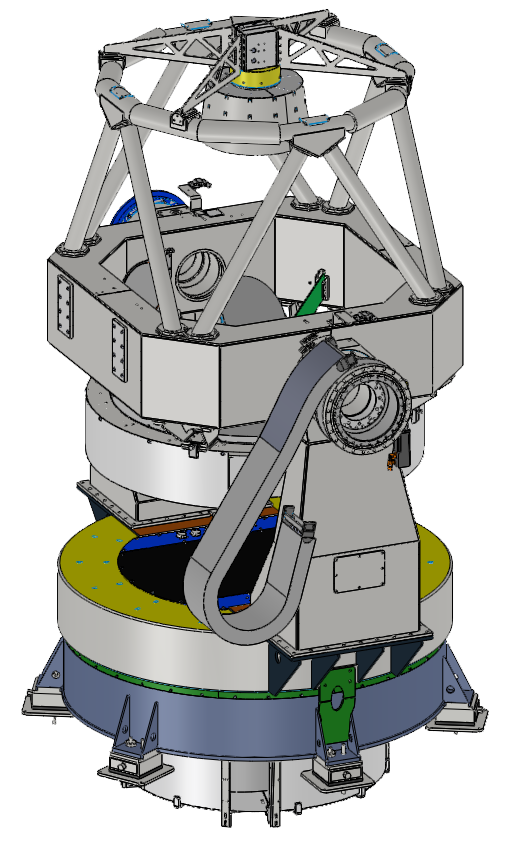
\includegraphics[width=0.8\linewidth]{newfigures/FigTel.png}
\end{center}
\caption{The COLIBRÍ Telescope}
\label{figure:alex-telescope-a}
\end{figure}

\begin{figure}
\begin{center}
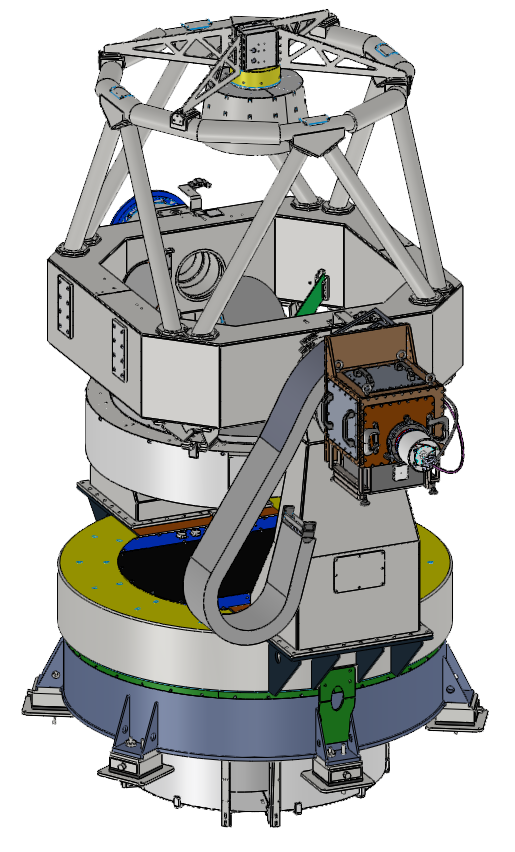
\includegraphics[width=0.8\linewidth]{newfigures/FigTelDDIN.png}
\end{center}
\caption{The COLIBRÍ Telescope and DDRAGO Interim Instrument}
\label{figure:alex-telescope-b}
\end{figure}

The reference origin of the instrument for structural design is at the intersection of the optical axis and the derotator flange.

\clearpage
\section{Support Structure}

\subsection{Design}

%\TODO{Lifting eyes on the SS?}
%
%\TODO{Describe support for RET1.}

\subsubsection{General Principles}

The design of the support structure for DDRAGO interim instrument is a simplification of the design we presented at the Conceptual Design Review in June 2016 and Preliminary Design Review in February 2017. The major simplification is to accommodate only one channel (corresponding to the blue channel) and to unfold its optics into a straight line, avoiding the reflections from D1 and D2. The science group, the optical designers, and mechanical designers worked together to refine this design through several iterations.

In our experience, for a compact instrument one of the best options for the support structure is using plates. This gives excellent stiffness but also allows us to use pin-holes in the plates as references for placing optical components. We built the warm part of the RATIR instrument according to these ideas, and the result was successful.

Our design uses 15 mm thick plates of Alumold 500 (although an equivalent 7000-series alloy could be substituted if need be). Alumold 500 is suitable for precision machining. We have used relatively large and continuous plates, with cut-outs where necessary, to give stiffness. The plates will be attached to each other using M8 bolts and threaded steel inserts. The manufacturing tolerances for these holes is good enough to guarantee the feasibility for assembling the structure and the subsystems.

The support structure has removable covers to allow the installation and calibration of all optical and electronic components of the instrument.

%\TODO{All removable plates need handles to ease their manipulation.}

\subsubsection{Complete Support Structure}

Figure~\ref{figure:alex-supported-components} shows the main components that are supported by the DDRAGO interim support structure.

Figure~\ref{figure:alex-complete} shows the complete support structure and all of the supported components.

Figure~\ref{figure:alex-ss-exploded} shows the support structure plates. We classify the plates as fixed (DR-ME-IN-FP$n$) and removable (DR-ME-IN-RP$n$).

Figure~\ref{figure:alex-support-plates} shows only the plates that support the components from Figure~\ref{figure:alex-supported-components}.

\begin{figure}[p]
\begin{center}
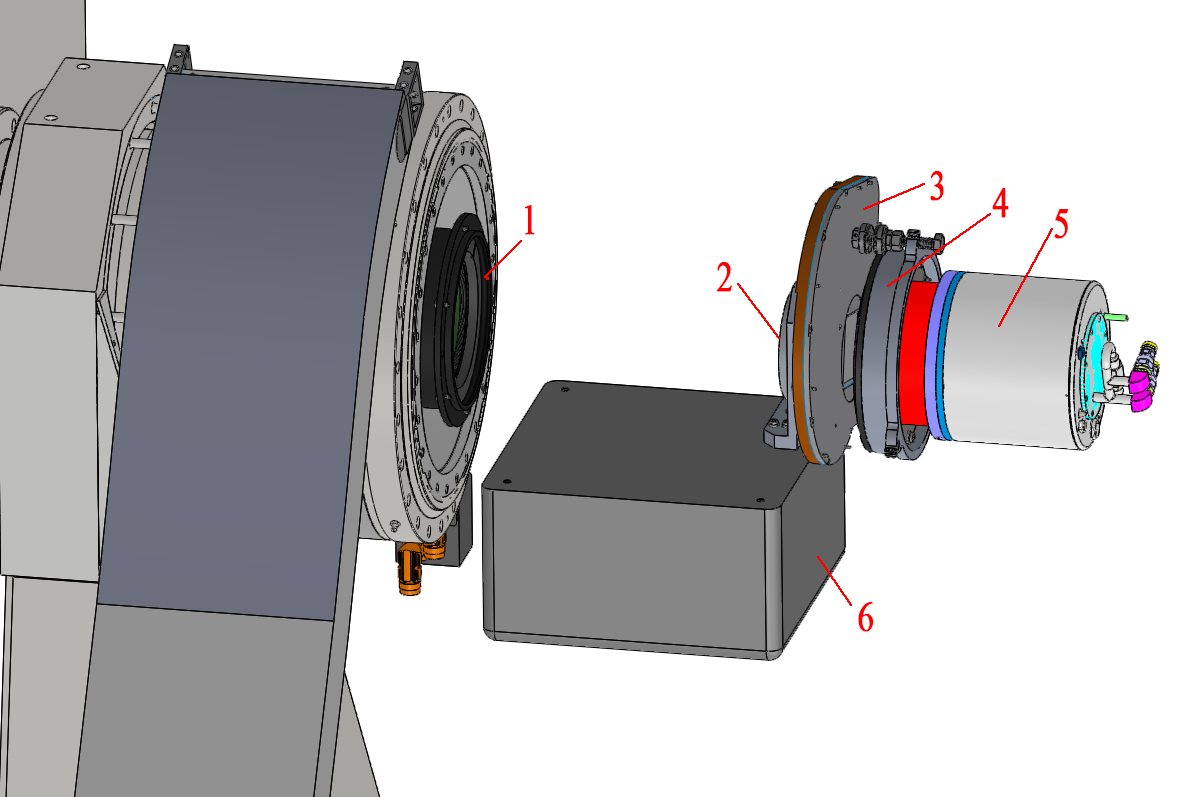
\includegraphics[width=\linewidth]{newfigures/Fig3_1.png}
\end{center}
\caption[The Supported Components]{The Supported Components. 1: The L1+L2 barrel (DR-ME-OML1L2), 2: the L3 mount (DR-ME-OML3), 3: the blue filter wheel (DR-ME-BFW), 4: the blue detector mount (DR-ME-OMBDET), 5: the blue detector (BDET) and 6: the close electronics (CE).}
\label{figure:alex-supported-components}
\end{figure}

\begin{figure}[p]
\begin{center}
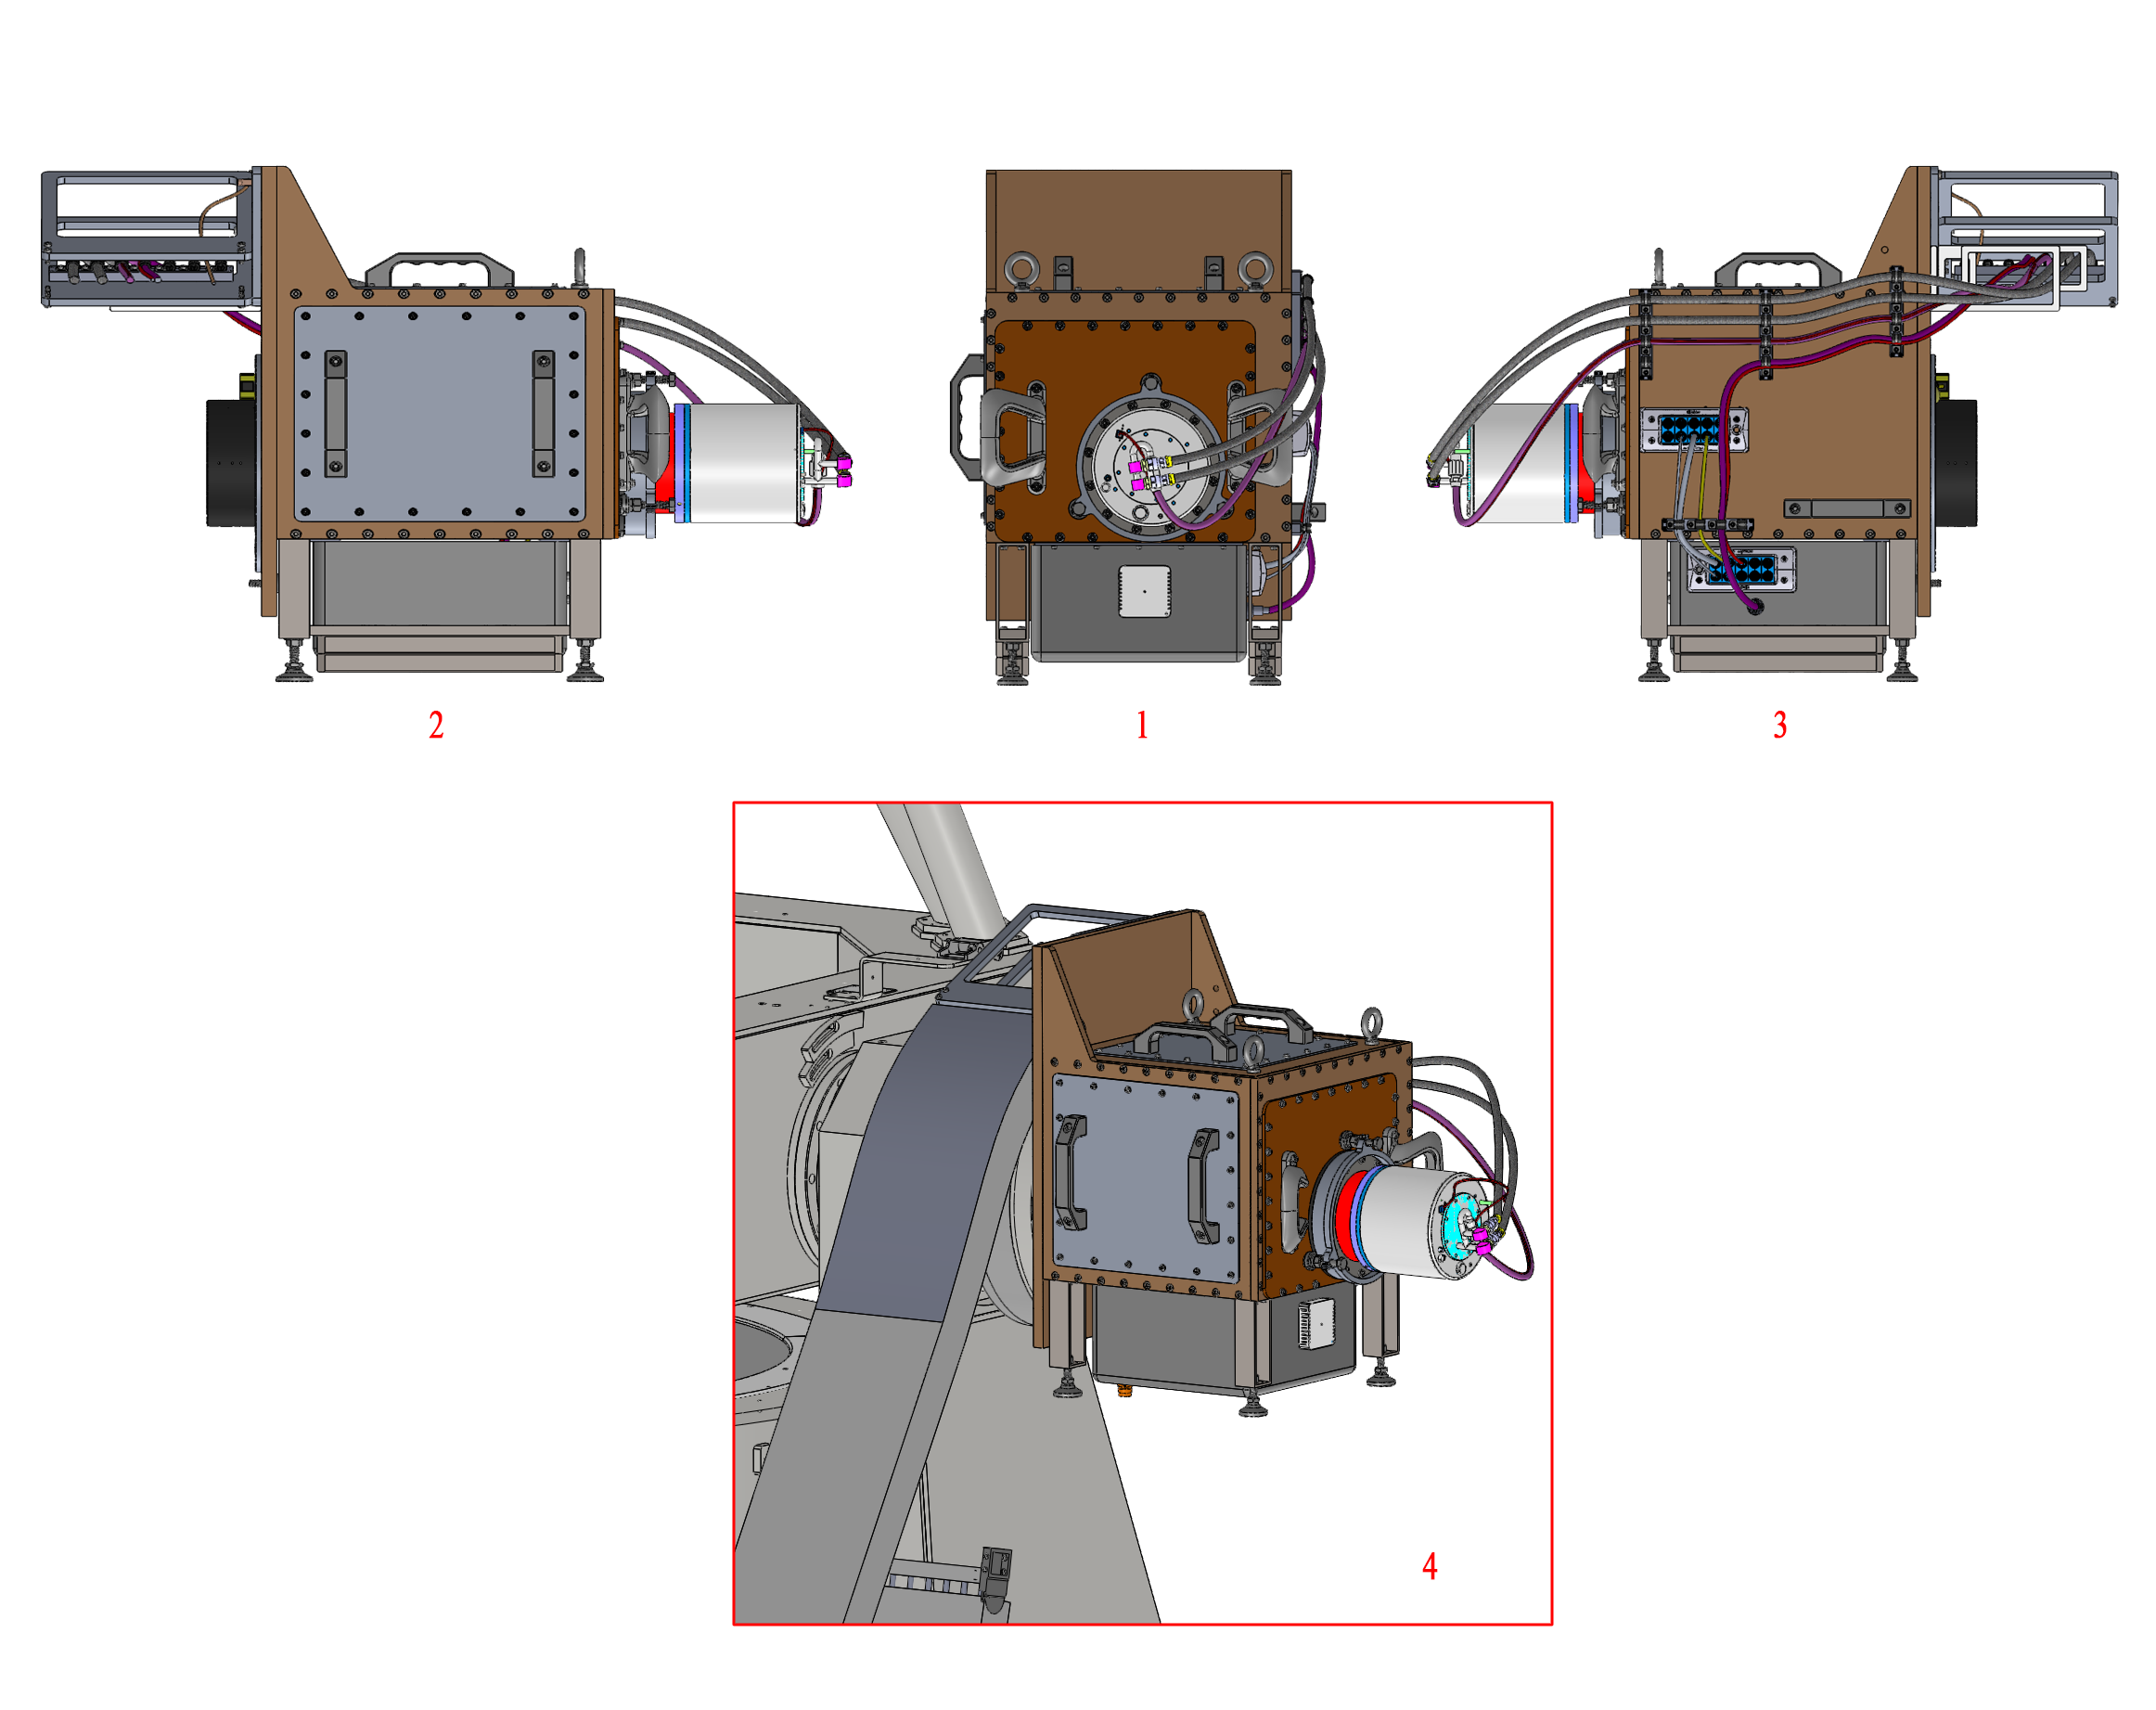
\includegraphics[width=\linewidth]{newfigures/Fig3_2.png}
\end{center}
\caption[The Complete Interim Support Structure and the Components it Supports.]{The Complete Interim Support Structure and the Components it Supports.
%(a--c) Transverse and lateral views of the support structure including all DDRAGO and CAGIRE components. (d) 3D view of the support structure including only the DDRAGO components. (e) 3D view of the support structure including all DDRAGO and CAGIRE components. The designs of the CAGIRE cryostat and close electronics are preliminary; we presume the final version of the close electronics will have a closed cabinet.
}
\label{figure:alex-complete}
\end{figure}

\begin{figure}
\begin{center}
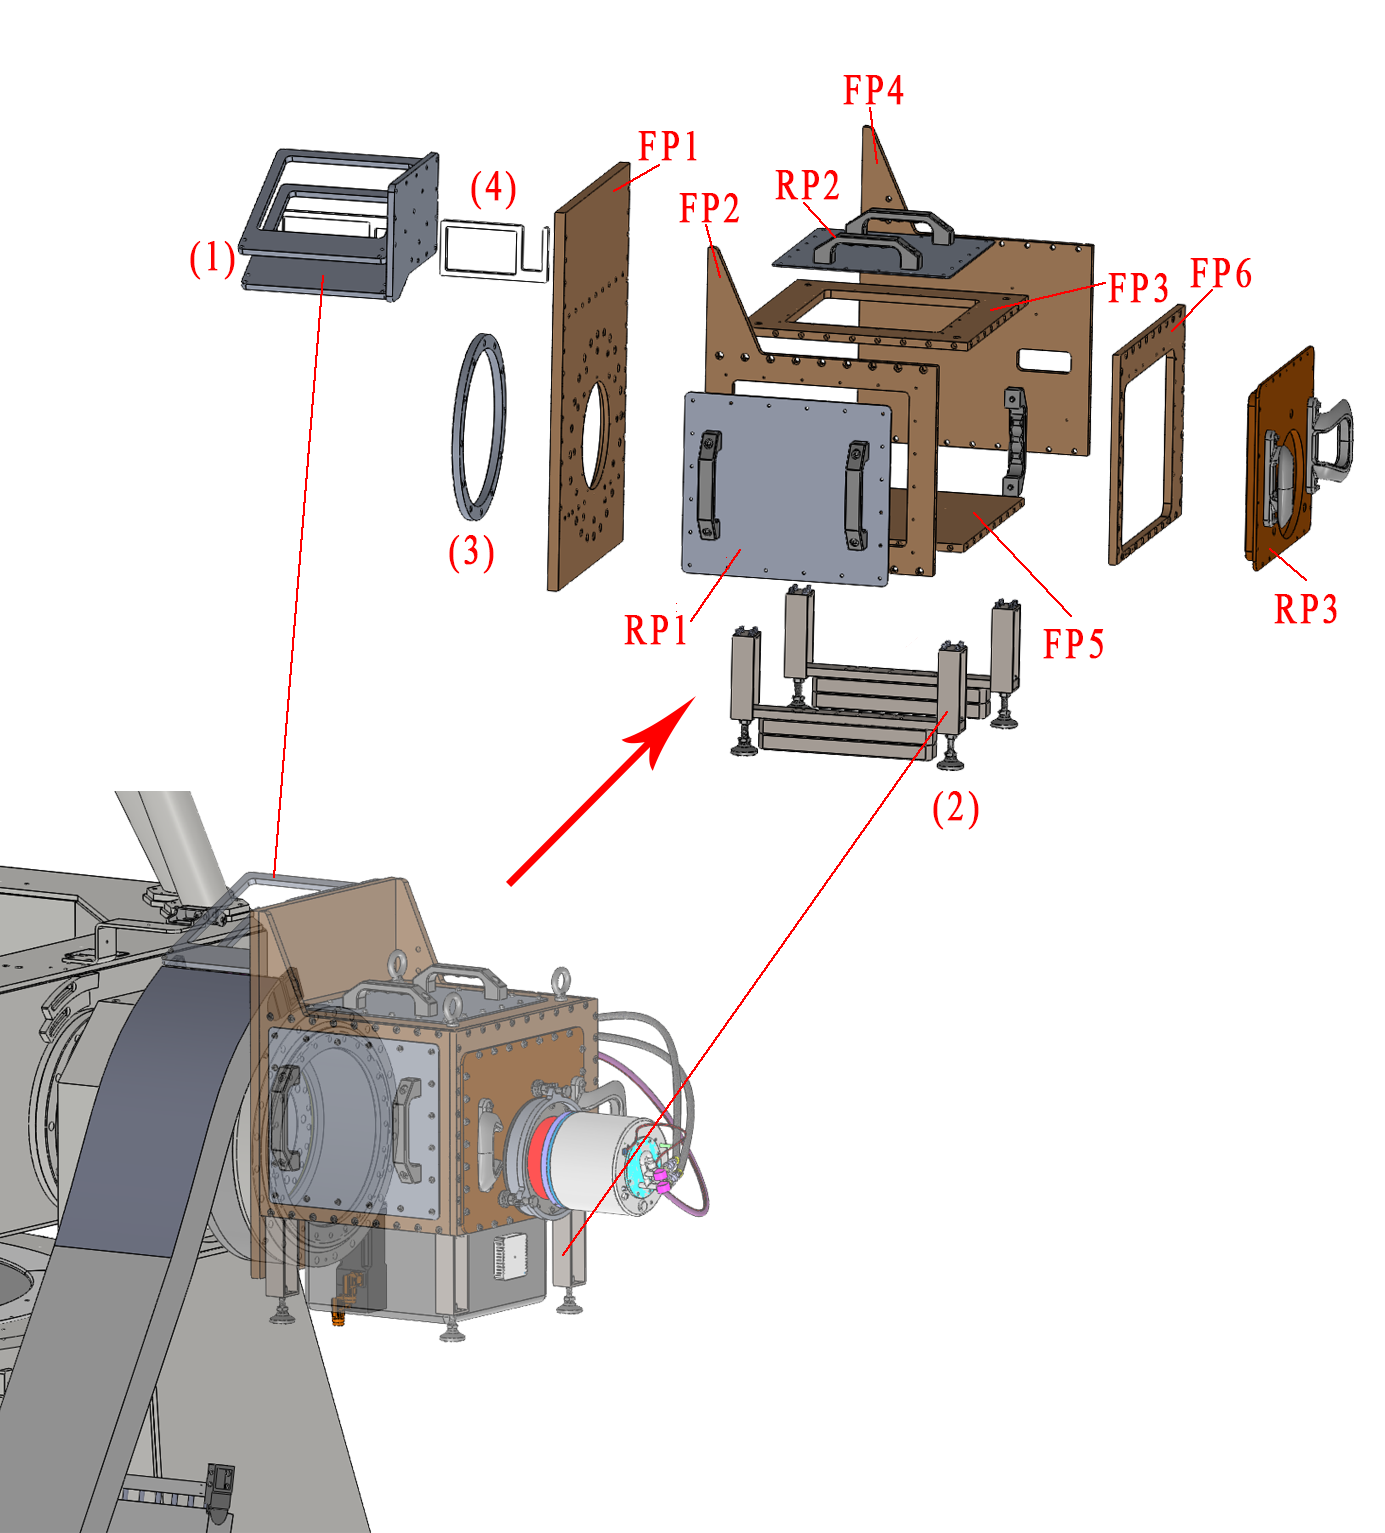
\includegraphics[width=\linewidth]{newfigures/Fig3_3.png}
\end{center}
\caption[The support structure plates.]{The support structure plates. In addition to the labelled plates, (1) is the cable wrap support (CWS), (2) are the support legs (SL1/2/3/4), (3) is the centering ring, and (4) is cable support guide (CSG).}
\label{figure:alex-ss-exploded}
\end{figure}

\begin{figure}
\begin{center}
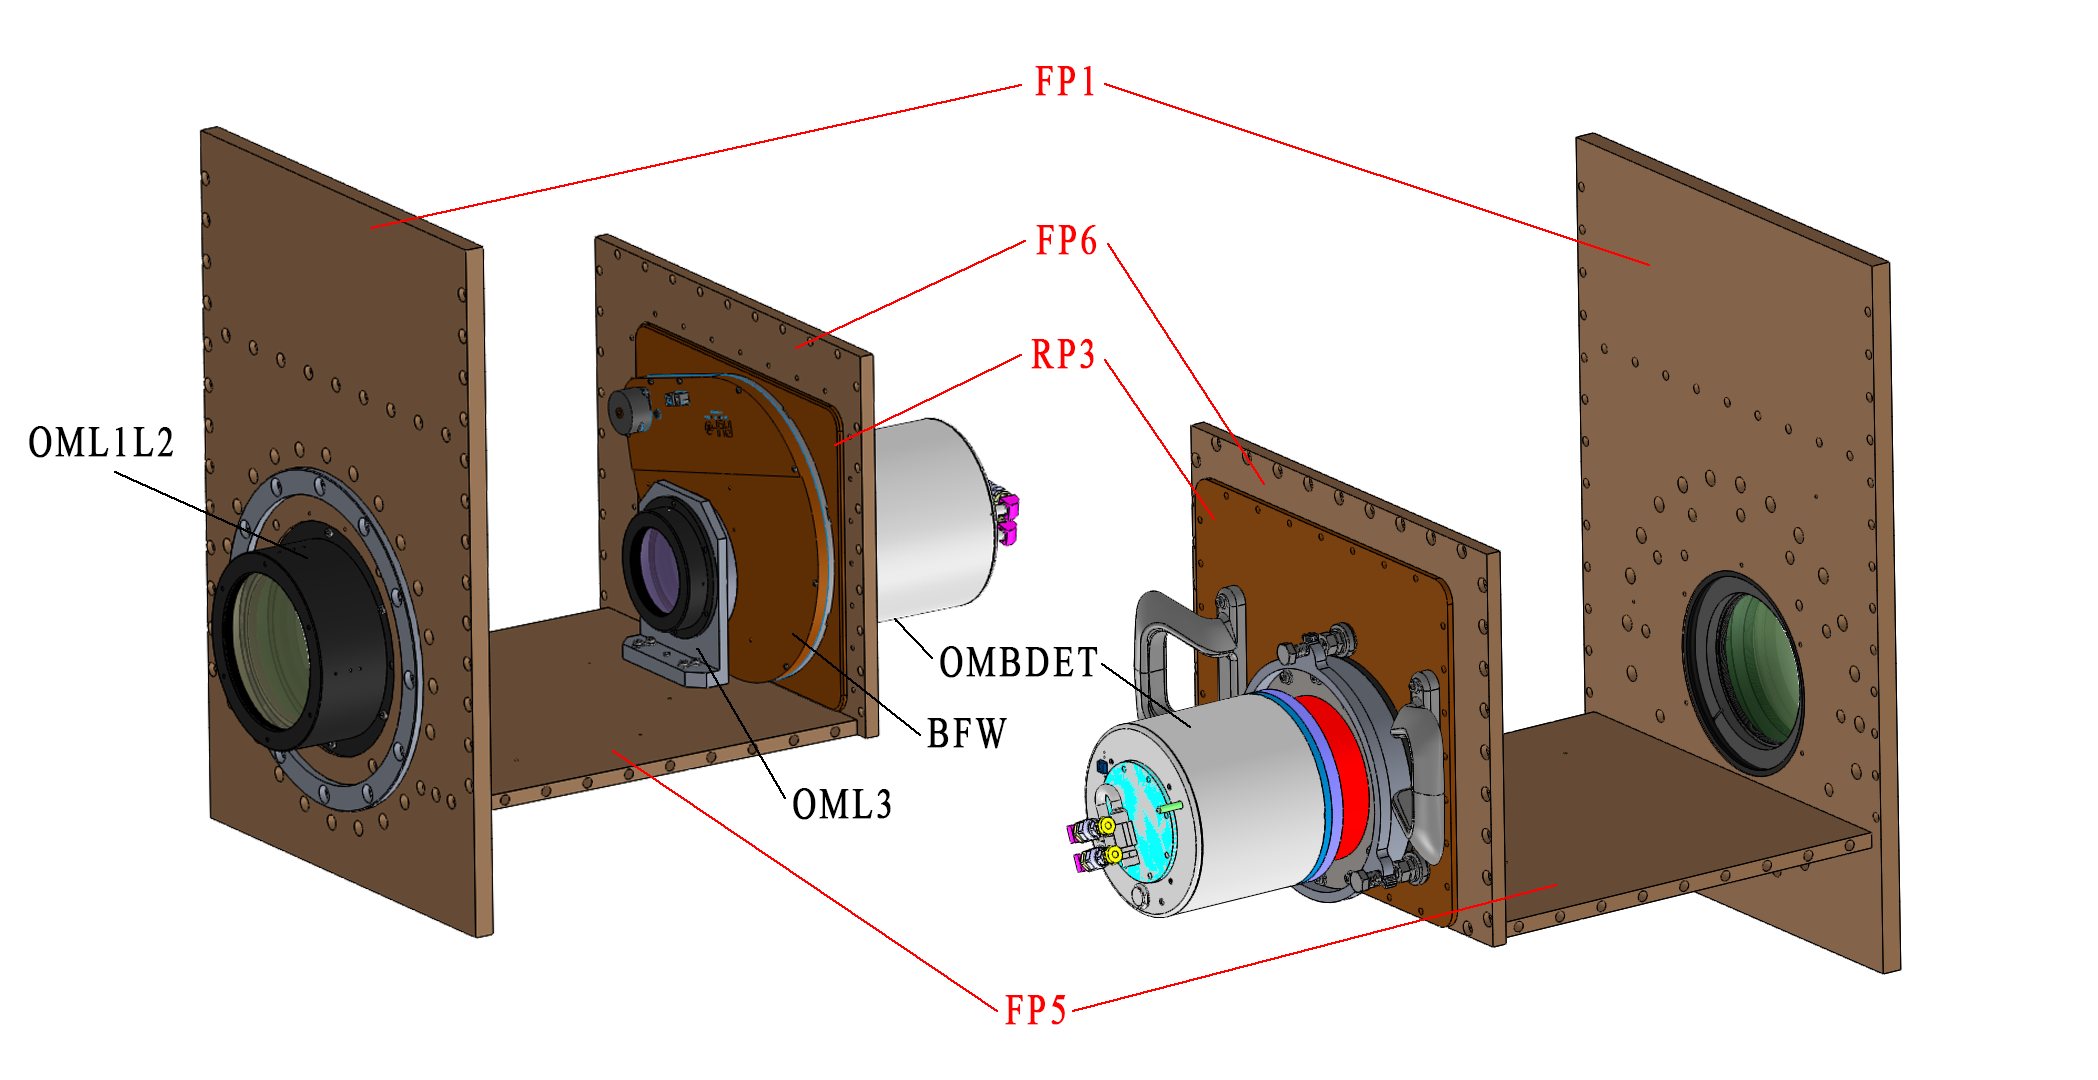
\includegraphics[width=\linewidth]{newfigures/Fig3_4.png}
\end{center}
\caption{The plates that support the optomechanical components.}
\label{figure:alex-support-plates}
\end{figure}


\subsubsection{Fixed Plate DR-ME-IN-FP1}

The front fixed plate DR-ME-IN-FP1, shown in Figure~\ref{figure:alex-ss-fp1}, is the interface between the telescope derotator and the instrument. Alignment with the derotator is achieved with the centering ring (DR-ME-IN-SR). The ring is 50 {\micron} undersized with tolerance h5 and so with the H6 tolerance on the derotator the final margin will be between 60 and 103 {\micron}.

The DR-ME-IN-FP1 plate also supports the optomechanical barrel for the doublet L1+L2 (DR-ME-OML1L2) and the cable wrap. The latter is divided in the actual cable wrap (CW), the cable wrap support (DR-ME-IN-CWS) and the cable support guides (DR-ME-IN-CSG1/2).

\begin{figure}
\begin{center}
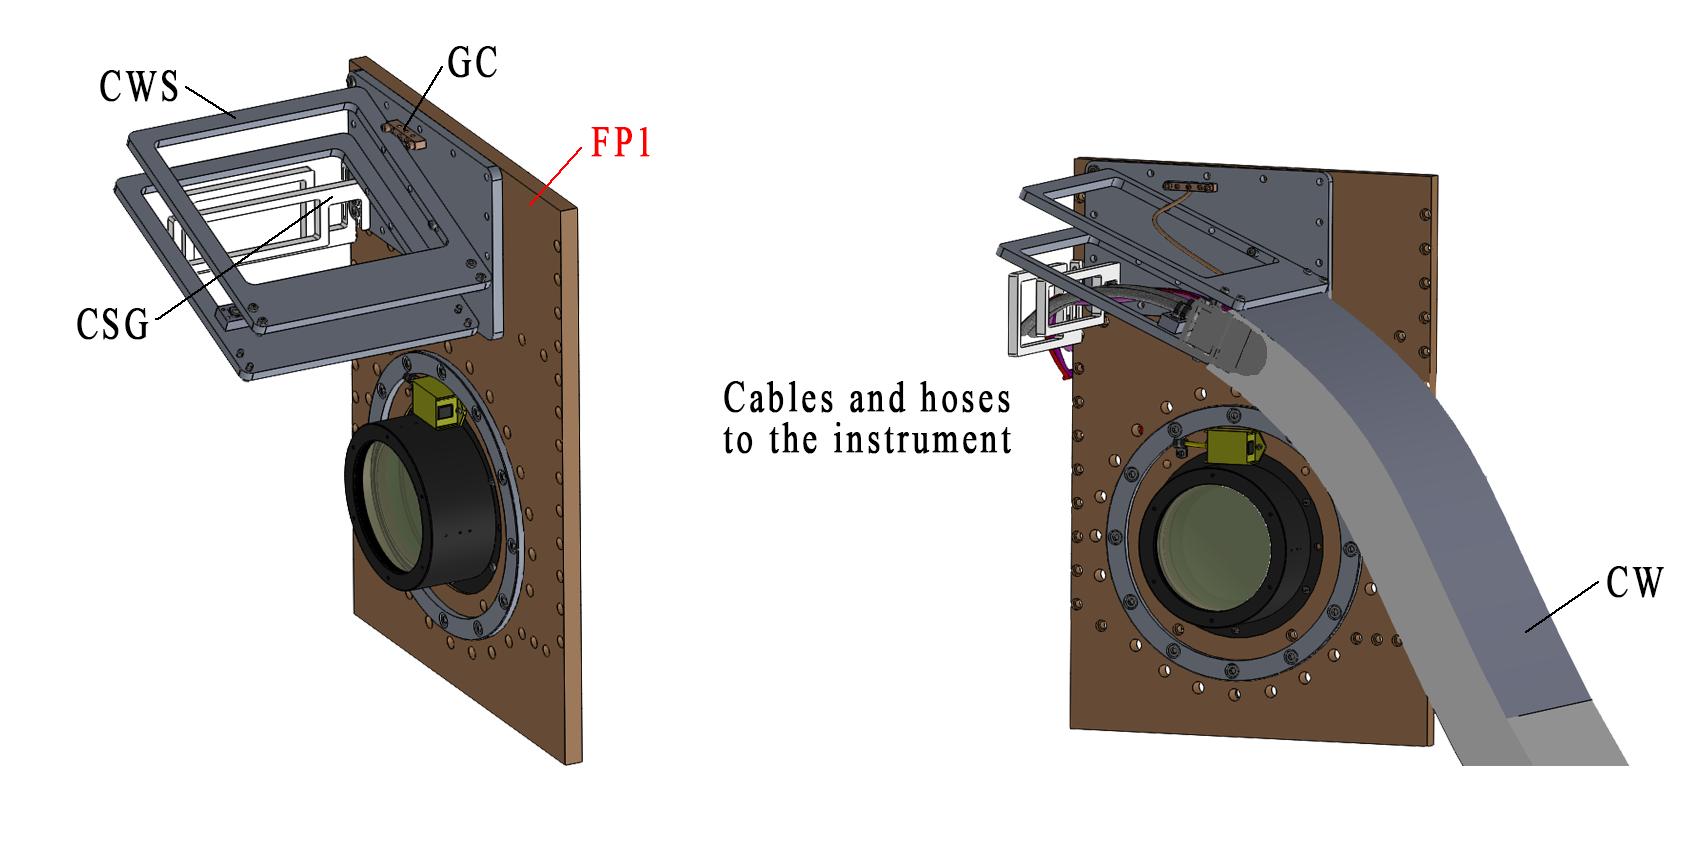
\includegraphics[width=\linewidth]{newfigures/Fig3_5.png}
\end{center}
\caption{The Support Structure Plate DR-ME-IN-FP1}
\label{figure:alex-ss-fp1}
\end{figure}

\subsubsection{Fixed Plate DR-ME-IN-FP5}

The bottom fixed plate DR-ME-IN-FP5, shown in Figure~\ref{figure:alex-ss-fp5}, supports the optomechanical mount of the lens L3 (DR-ME-OML3) and the close electronics (DR-CO-CE), and has four legs (DR-ME-IN-SL1/2/3/4) for when the instrument is not on the telescope. The close electronics cabinet for the DDRAGO interim instrument will be attached to the fixed plate DR-ME-IN-FP5 using two custom supports (DR-ME-IN-CES1/2).

\begin{figure}
\begin{center}
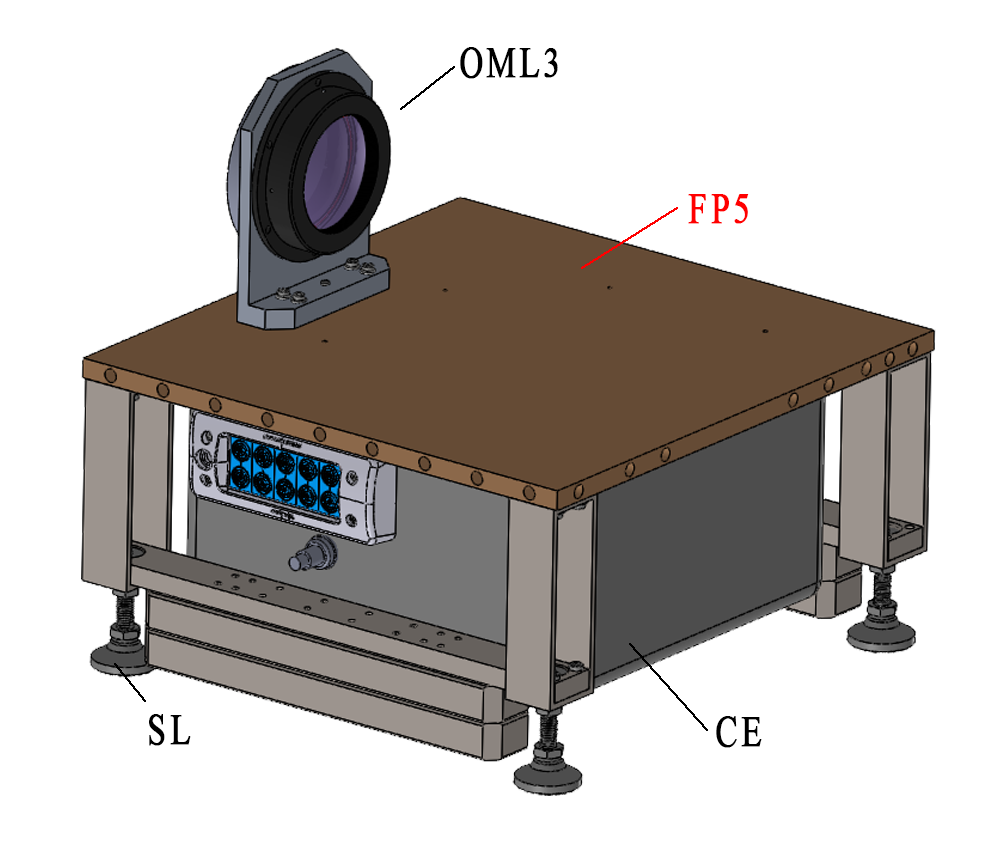
\includegraphics[width=0.6\linewidth]{newfigures/Fig3_6.png}
\end{center}
\caption{The Support Structure Plate DR-ME-IN-FP5.}
\label{figure:alex-ss-fp5}
\end{figure}

\subsubsection{Fixed Plate DR-ME-IN-FP6 and Removable Plate DR-ME-IN-RP3}

The back fixed plate DR-ME-IN-FP6, shown in Figure~\ref{figure:alex-support-plates}, supports the blue detector mount (DR-ME-OMBDET) and blue filter wheel (DR-ME-BFW), indirectly through the removable plate DR-ME-IN-RP3. 

The removable plate is mainly to provide access to the filter wheel, since the access the filter wheel from the inside of the instrument is very tight. The removable plate has two metal handles (McMaster part 1979A300) to ease its manipulation. The mass of RP3 with the detector and filter wheel is approximately 23~kg (of which about half is the CCD which can be removed first if need be).

%\TODO{Movement on RP3}

%\TODO{Blocking of RP3}

\subsubsection{Other Plates}

Plates DR-ME-IN-FP2, DR-ME-IN-FP2, and and DR-ME-IN-FP4 (see Figure \ref{figure:alex-ss-exploded}) are the lateral and top plates and do not support any optomechanical components, although FP4 does support cables.

The lateral plate DR-ME-IN-FP2 has the removable plate DR-ME-IN-RP1 for  access to the instrument. The removable plate has two nylon handles (McMaster part 5193A400) to ease its manipulation. The mass of the removable plate is about 2.5~kg.

The top plate DR-ME-IN-FP3 has the removable plate DR-ME-IN-RP2 for access to the instrument. The removable plate has two nylon handles (McMaster part 5193A400) to ease its manipulation. The mass of the removable plate is about 2.5~kg. The plate also has four M12 steel lifting eyebolts (McMaster part 3040T150) for attaching a lifting harness. Each eyebolt is capable of supporting a vertical load of 1000 kg.

The lateral plate DR-ME-IN-FP4 has a hole for the RoxTec CM 20w40 cable seal. Although FP4 is fixed, it also has an nylon handle (McMaster part 5193A400) to easy maneuvering the instrument on a crane, for example.

\subsubsection{Legs and Feet}

The four leg columns DR-ME-IN-SL1/2/3/4 are cut from stainless steel rectangular tube (McMaster part 89825K72) and are fitted with four feet DR-ME-IN-SL1/2/3/4-FT (McMaster part 6120K490). The leg columns also are used to support the steel counterweights. We estimate we need about 16~kg of counterweights to balance the instrument, but we will supply more and will supply different masses of counterweight to aid precise balancing.

\subsection{Manufacture and Assembly}

The support structure plates will be manufactured using CNC techniques. 
We have a CNC machine in the Instituto de Astronomía, but it is limited to pieces no larger than about $300 \times 300 \times 250$~mm. The support structure plates are larger and will have to be manufactured externally. We have identified a suitable commercial workshop in Mexico City.

Using standard CNC techniques, a typical precision for the holes is 100~{\micron}/m. This is sufficient that we can satisfy the optical tolerances on position by manufacture. 

We note that there are two classes of bolt holes in the support structure: \emph{precision} ones to assemble the support structure and to attach the optomechanics and \emph{non-precision} ones to attach components such as cables, electronic boxes, sensors, and counter-weights. 

We intend to place the contract for the external fabrication of the plates in the first week of June 2018. For this point, we need to have defined all of the precision bolt holes. We can add additional non-precision bolt holes later using conventional machining techniques. Obviously, though, it would be convenient to have as many of the bolt holes as possible fabricated externally.

Figure~\ref{figure:alex-bolts} shows the plates array of the support structure with bolts.

The verifications process of the support structure will validate the dimensions of the array prior to assembly and dimensions, perpendicularity, and parallelism after assembly. 

The support structure is about $77 \times 46 \times 47$~cm. This is small enough that we can use the Mitutoyo 7106 coordinate-measuring machine in the IA workshops to perform metrology of the entire structure. (The Mitutoyo 7106 accepts pieces up to $100 \times 70 \times 60$~cm.) 

Once the structure has been assembled and verified, all of the optomechanical supports can be integrated from outside.

\begin{figure}
\begin{center}
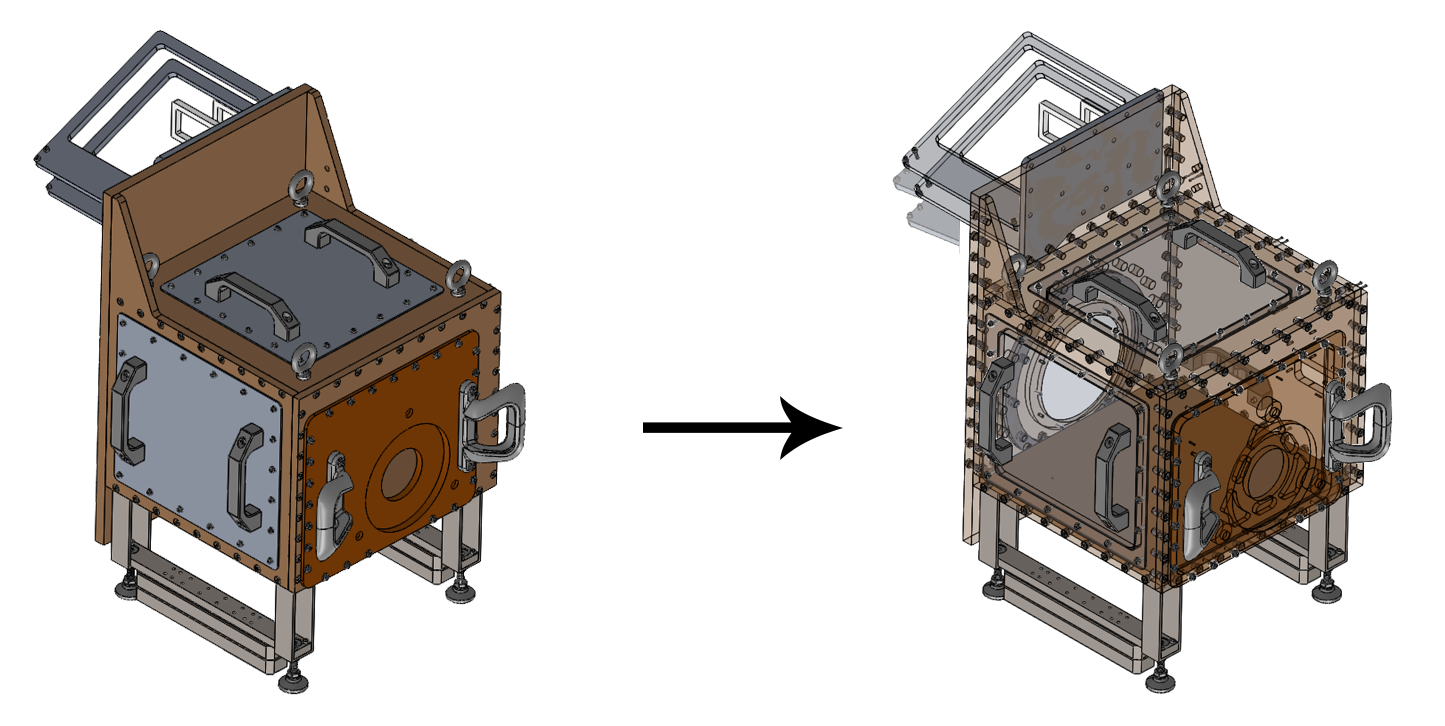
\includegraphics[width=\linewidth]{newfigures/Fig3_7.png}
\end{center}
\caption{The Bolts Used in the Support Structure.}
\label{figure:alex-bolts}
\end{figure}

\subsection{Displacements and Mechanical Stresses}

We have not explicitly studied the displacements and mechanical stresses in the structure. However, we did study these for the similar, but much heavier and larger, structure we designed after CDR and found that they were negligible compared to the tolerances on the positions of the optical components. Therefore, we are confident that in this lighter, smaller, and more rigid structure that they will also be negligible.

%\TODO{Repeat this analysis with the weights necessary to move the COM to the derotator axis. However, we are so far within the tolerances, that we are confident that this will make no significant difference.}
%
%\begin{figure}
%\begin{center}
%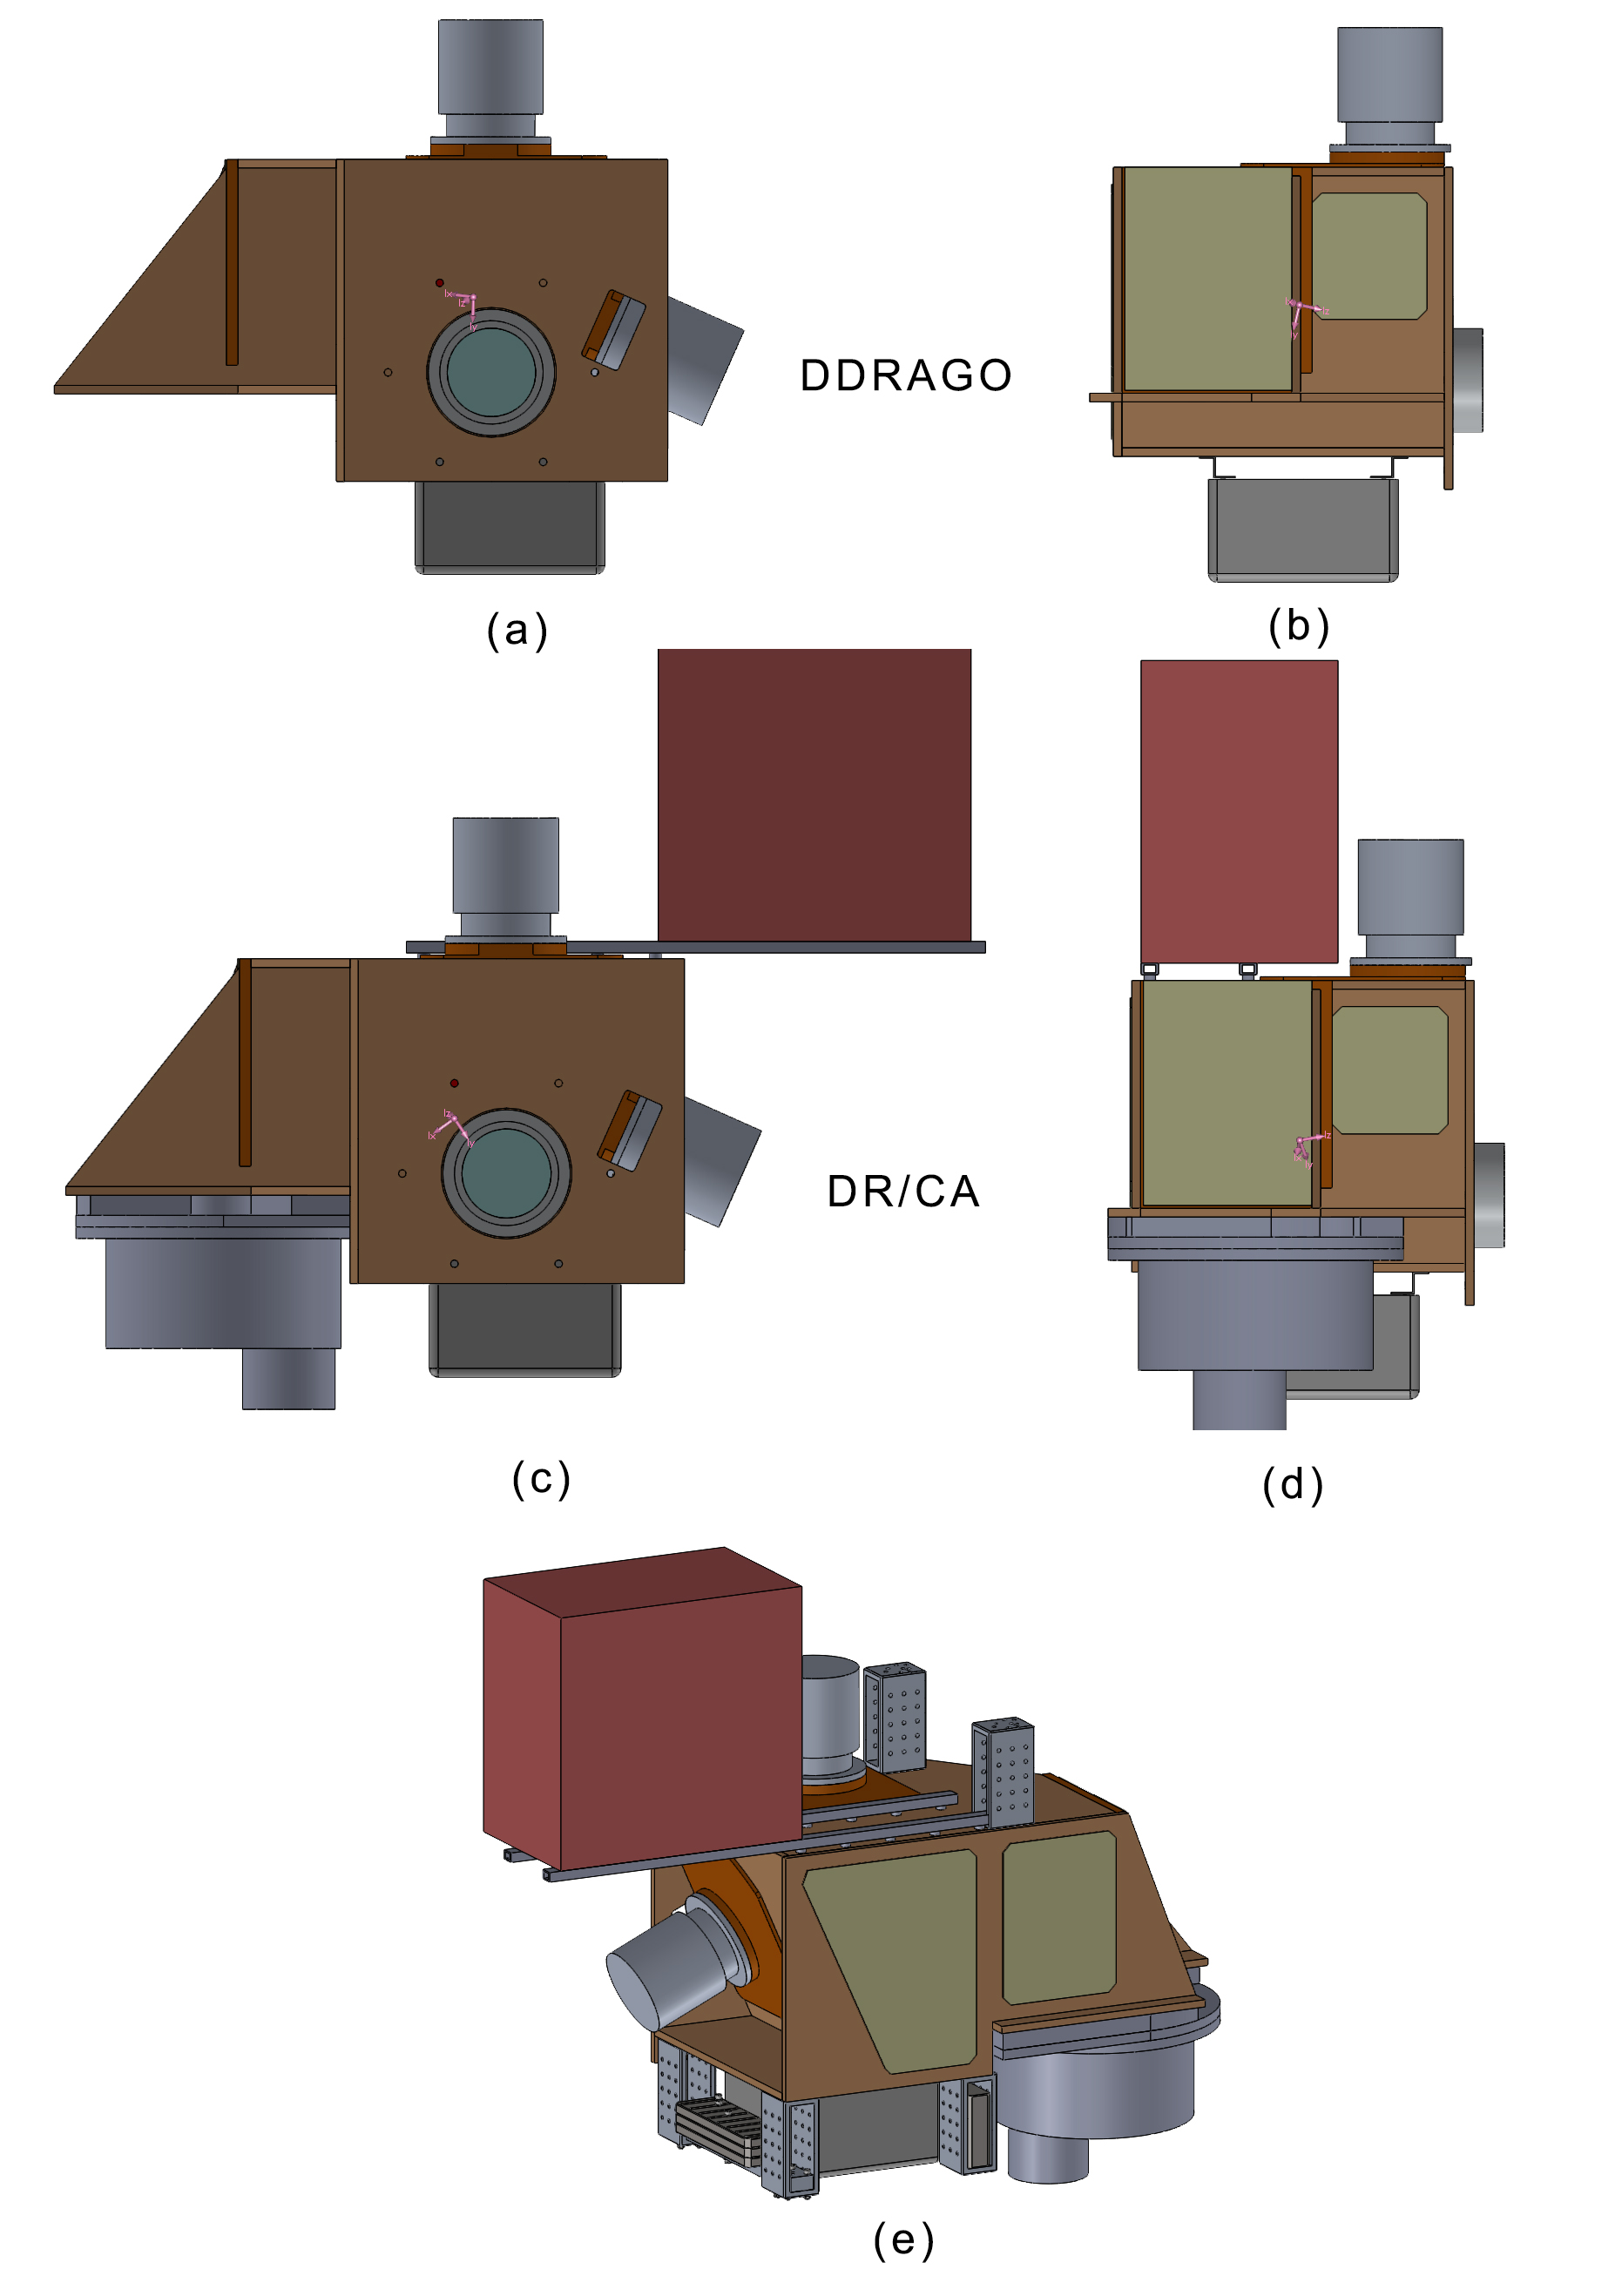
\includegraphics[width=\linewidth]{figures/alex-simplified-model.jpg}
%\end{center}
%\caption{Simplified Model for Finite-Element Analysis.}
%\label{figure:alex-simplified-model}
%\end{figure}
%
%\begin{figure}
%\begin{center}
%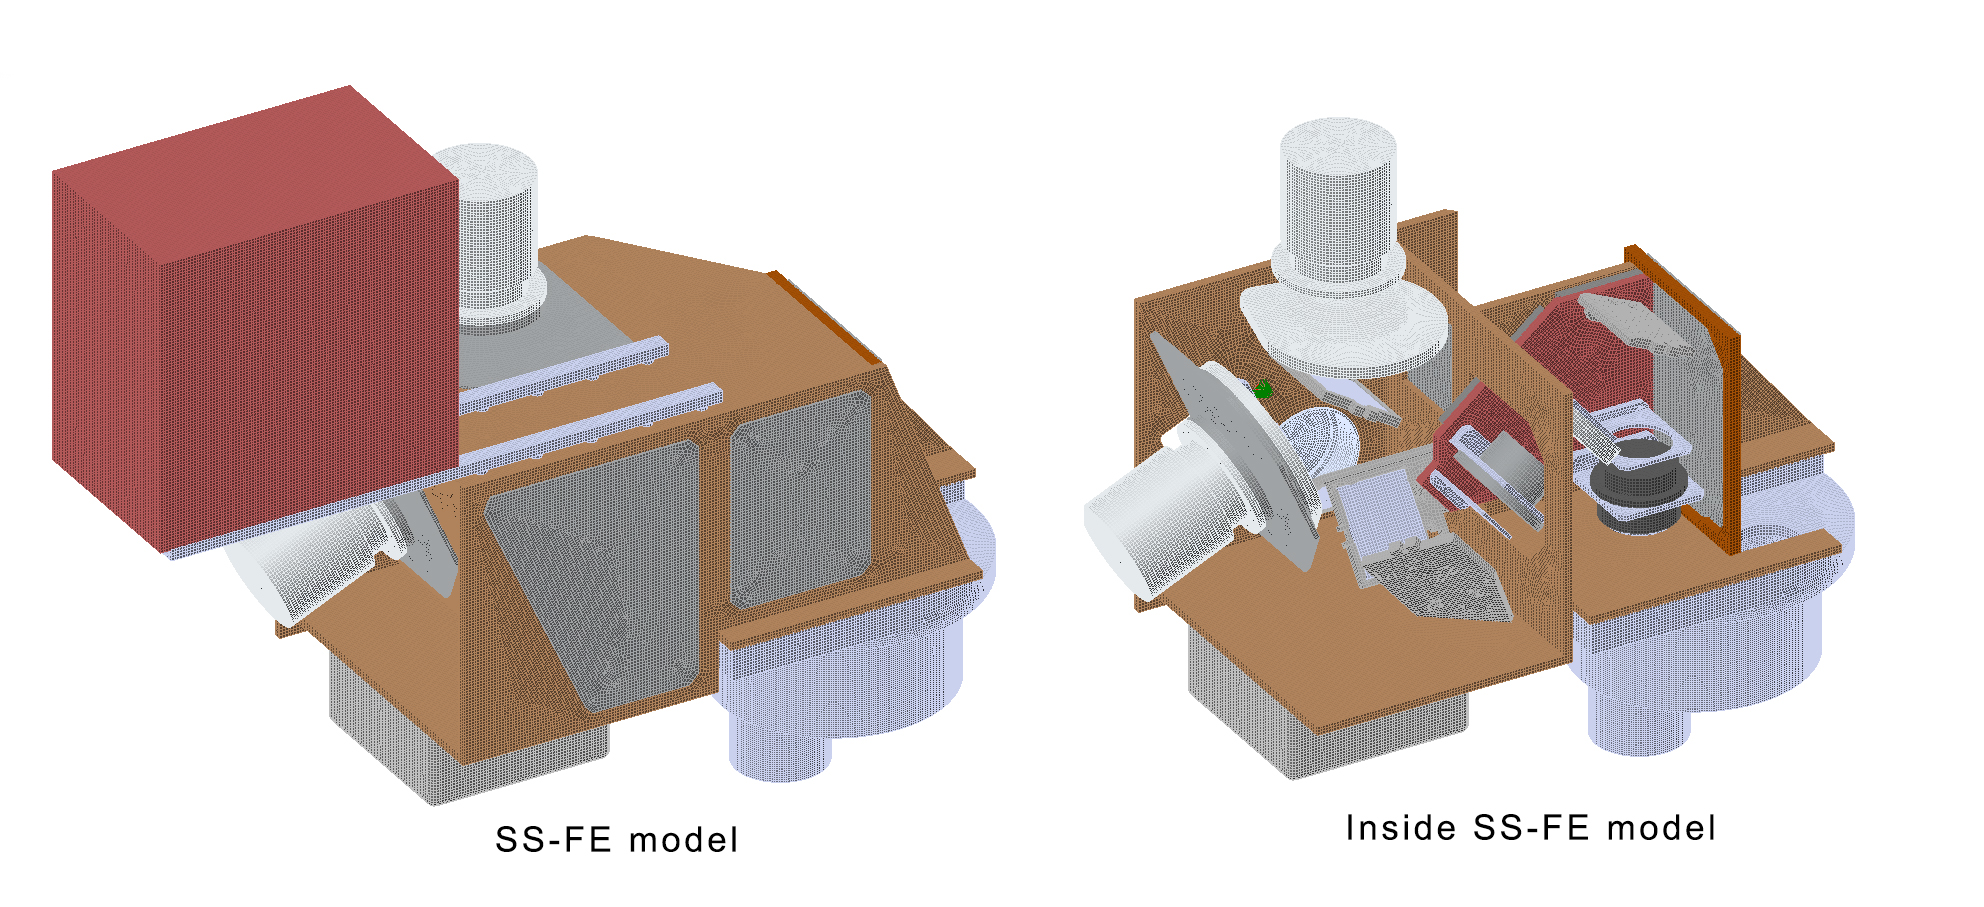
\includegraphics[width=\linewidth]{figures/alex-mesh.jpg}
%\end{center}
%\caption{The Finite-Element Analysis Mesh.}
%\label{figure:alex-mesh}
%\end{figure}
%
%\begin{figure}
%\begin{center}
%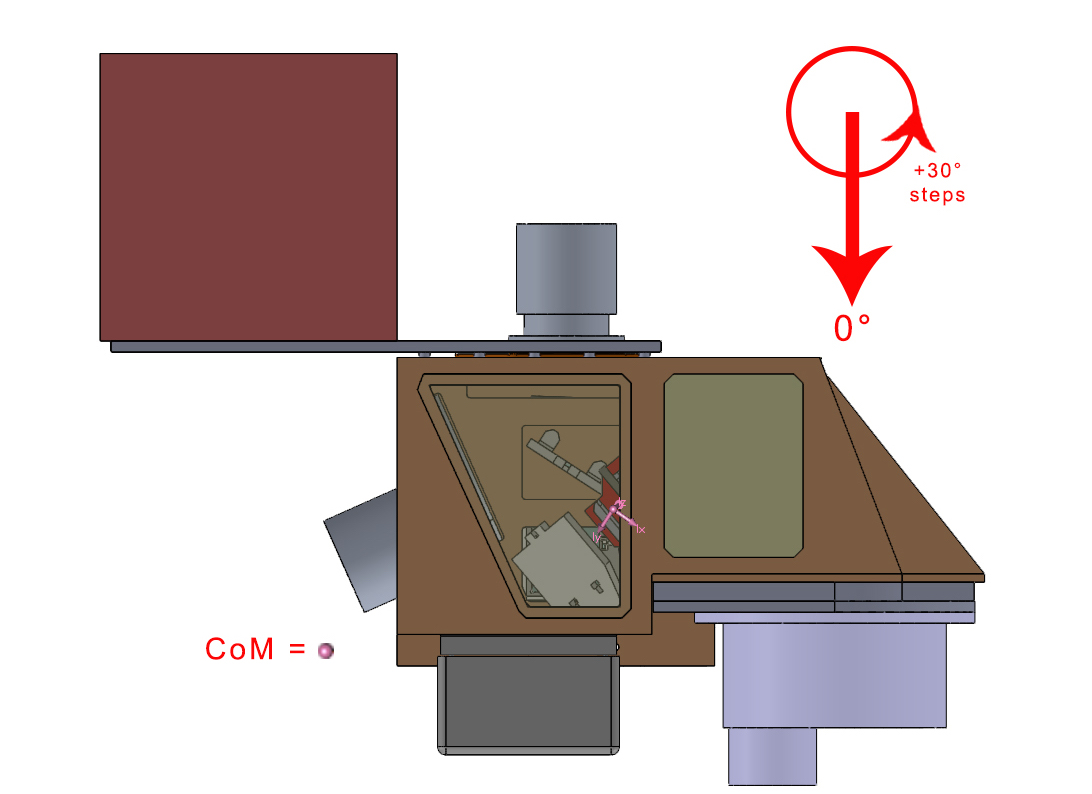
\includegraphics[width=\linewidth]{figures/alex-gravity.jpg}
%\end{center}
%\caption{The Variable Gravity Vector.}
%\label{figure:alex-gravity}
%\end{figure}
%
%\begin{figure}
%\begin{center}
%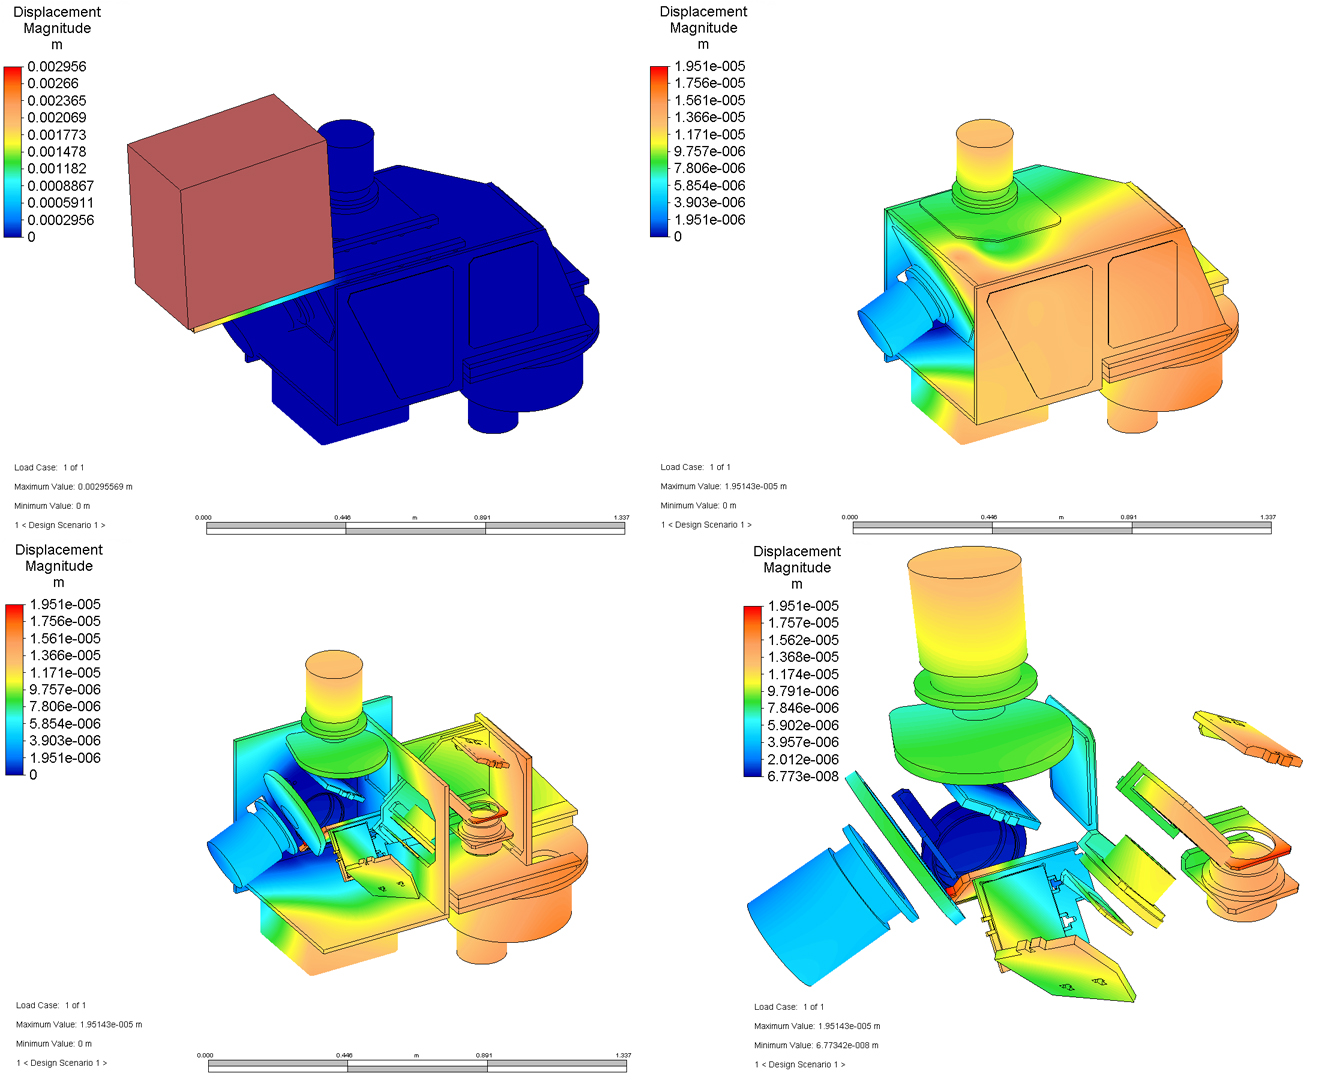
\includegraphics[width=\linewidth]{figures/alex-displacements.jpg}
%\end{center}
%\caption{The Displacements Under Gravity at 0 {\deg}.}
%\label{figure:alex-displacements}
%\end{figure}
%
%From the detailed model, we created a simplified model of the support structure and the optomechanical components for finite-element analysis. The simplified model is shown Figure~\ref{figure:alex-simplified-model} and the finite-element mesh is shown in Figure~\ref{figure:alex-mesh}.
%
%We then determined the distortion of the support structure and the displacements of the optomechanical elements as gravity varied. As Figure~\ref{figure:alex-gravity} shows, we varied the gravity by 30 {\deg} through a complete rotation on the derotator. Figure~\ref{figure:alex-displacements} shows the displacements under gravity at one position. The largest displacement at any rotation (with respect to zero gravity) is less than 20~{\micron}. The displacements are dominated by deformation of the interface plate DR-ME-IN-FP1 to the derotator; the rest of the structure behaves much more rigidly. The tilt of the instrument with respect to the derotator corresponds to approximately $0.002$ {\deg} (7~{\arcsec}). We have verified that the displacements are all small compared to the tolerances in position derived from the optical design.
%
%The stresses in the structure are sufficiently small that they fulfill the von Mises criterion. Therefore, we do not expect any mechanical failure.

%\subsection{Accessibility}
%
%\begin{figure}
%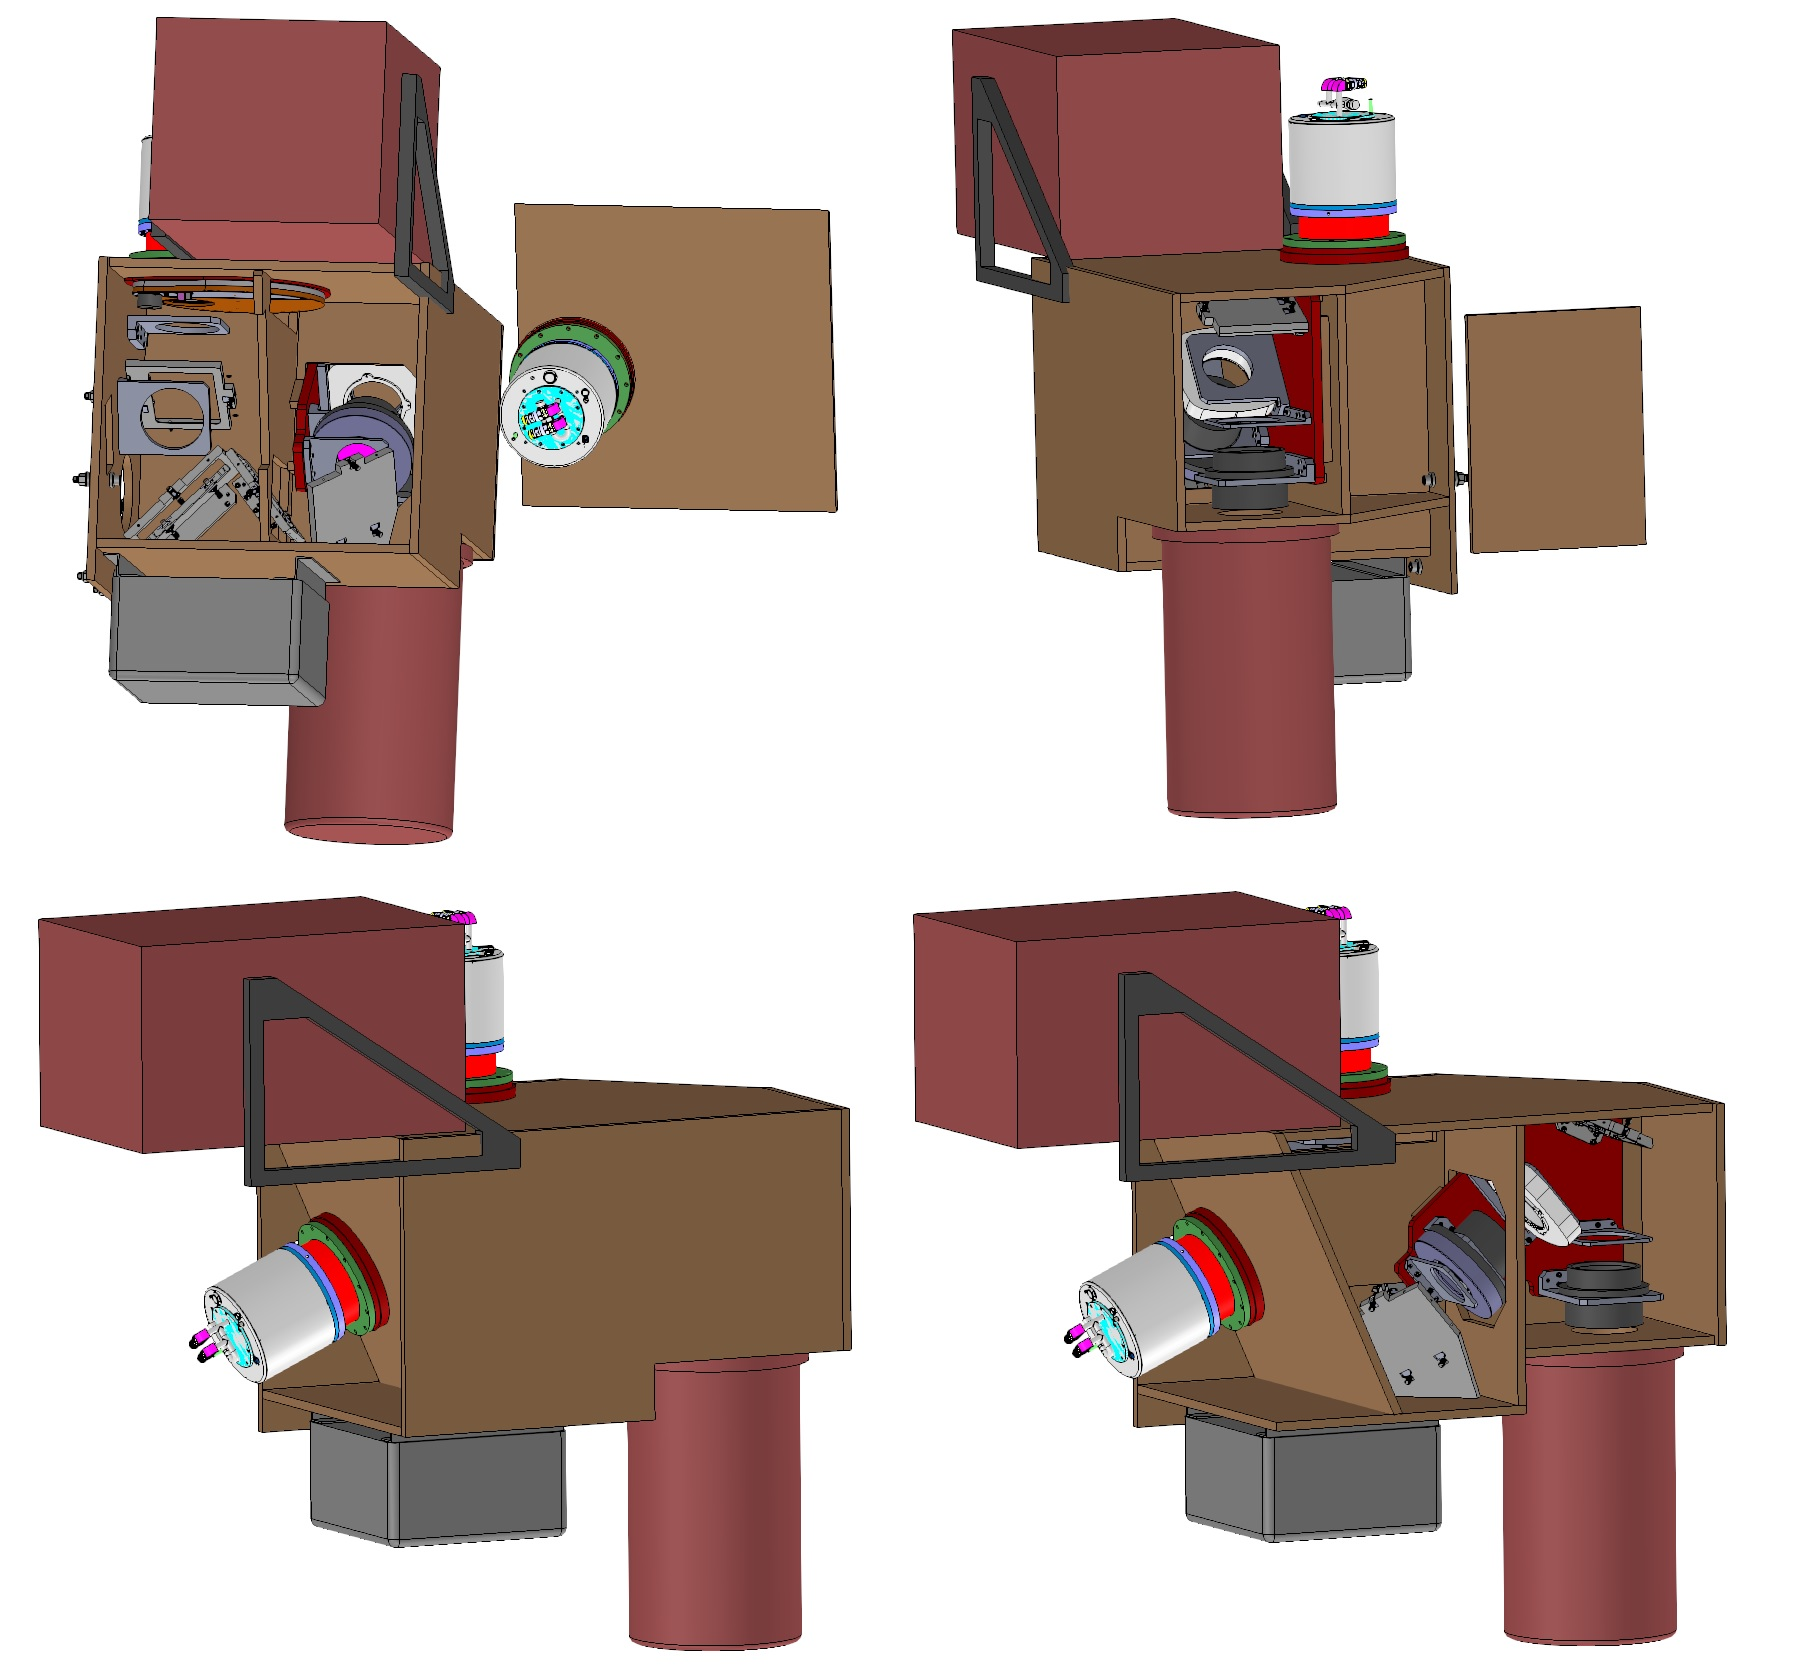
\includegraphics[width=\linewidth]{figures/alex-16.jpg}
%\medskip
%\caption{Access to the Components in the Support Structure}
%\label{figure:alex-16}
%\end{figure}
%
%Alignment and maintenance will require access to the components mounted within the support structure. Figure~\ref{figure:alex-16} shows how we might achieve this access by dismounting individual plates. During the detailed design, we will make sure that the mechanical interferences and ergonomic problems are solved.
%
%All removable plates will have handles to ease their manipulation.

%\subsection{Ventilation}
%
%An earlier version of the FPRD required us to maintain the temperature within the support structure within 1 C of the ambient temperature, in order to avoid “instrument seeing”.
%
%This is somewhat difficult to achieve while still safeguarding the physical safety of the optics against dust and humidity. We have considered a passive solution that has two or more ventilation openings, without fans but with particle filters and light traps. We could guard against humidity by installing a hygrometer-activated heater that turns on at 95\% humidity.
%
%As the FPRD evolved, this requirement was removed. We arrived at the decision that we will initially not implement this passive solution, but will instead leave it as a possible upgrade. That is, we will design this system (ventilation and heating) and add the ventilation openings to the support structure. However, at least initially, we will close the ventilation openings with plates. If metrology from the temperature sensors in the support structure indicates that temperature gradients within the instrument are significant at the telescope, we will consider implementing the upgrade. Such a decision would be taken in consultation with the GFT project and the OAN.


\clearpage
\section{DDRAGO Lens Mounts}

%
%The optomechanical design refers to the positioning and fixation of the optical elements of DDRAGO/CAGIRE observing the optical specifications and contributing to achieving the goal of image quality. It takes into account as well, the instrument performance in the environment determined by the weather conditions at the OAN, the OHP, and the shipping conditions that the packed instrument will experience

%In this process the material selection, fabrication procedures and finish are adequately selected.

\subsection{Introduction}

Here we describe the optomechanical design proposed for the two lens mounts for the DDRAGO interim instrument: the common doublet L1+L2 (DR-ME-OML1L2 in the product tree) and the blue channel field singlet L3 (DR-ME-OML3).

The major change in the design from PDR is that we have changed the thermal compensator. In PDR, we proposed to use PTFE (Teflon) rings as the principal thermal compensator. However, as we developed this design we worried that precision PTFE rings, especially conical ones, would be difficult to manufacture. Therefore, we have now adopted silicone O-rings as the thermal compensator. (Simple PTFE rings are used to avoid friction between the aluminium O-ring holder and the aluminium preload ring, but they no longer require precise machining in thickness.)

%In the version 1.0 of this document, prepared for the PDR, we also presented a design for the L8+L9+L10 triplet from CAGIRE. The CAGIRE optomechanical supports have not been updated to use the new thermal compensator concept. Therefore, to avoid confusion, in this version we have omitted this and the other CAGIRE WOB lens mounts. (The optomechanical support for L11 is part of the cryostat work package being carried out by IRAP.)

We begin by summarizing the design considerations. We then present the designs, first in a general sense and then individually for DR-ME-OML1L2 and DR-ME-OML3. We then discuss the required preload, the thermal compensation, and the likelihood of failure due to stresses. (Birefringence is discussed in \ref{optics}.)

\subsection{Considerations}

The optomechanical design presented here was developed according to the following specifications established by the optical design:
\begin{enumerate}
\item
The lens materials are {\CaF}, N-BaK4, and fused silica.
\item The barrels should provide an attachment flange to allow them to be attached to the plates of the support structure (L1+L2) or to a precision L-brackets (L3).
\item The tolerances in axial positioning, decentering, and tilts are given by the optical design.
\item The alignment and verification of lenses inside their respective barrels will be carried out with the IA-UNAM aligning system ALBATROS (see \ref{aiv}).
\item Mechanical parts and lenses will be manufactured and integrated at a temperature of about 20~C
\item The operational temperature range is $-15$~C to 20~C.
\item The survival temperatures is from $-25$~C to 50~C.
\item The supports must protect the lenses and maintain their alignment against accelerations of $10g$.
\end{enumerate}

\subsection{Design}

\subsubsection{General Design}

The lens mounts will be manufactured from Alumold® 500 (or a similar 7000-series alloy). Alumold has been chosen for its ease of precision machining and excellent mechanical properties.

All of the barrels will have a flange for fastening to their corresponding structural brackets or plate. Their flange will provide the reference surface to locate the barrel in the correct position in the optical arrangement. The barrels are attached using are 316 Stainless Steel socket head screw low-profile (McMaster part 90666A124). The flange on the barrel for the L1+L2 doublet will be attached directly to the plate SS-FP1. The flange of the barrel for the L3 lens will be attached to a precision L-bracket which in turn is attached to plate IN-FP5. The L-bracket is attached using bolts for strength and smaller shoulder bolts to achieve the required tolerances by manufacture. 

Inside each barrel there is another reference surface designed to make contact with the polished convex surface of one of the lenses (L1 or L3) and to thereby maintain the lens in its correct position in the barrel. A precision aluminum spacer will be used to separate the lenses of the doublet L1+L2. This spacer will make contact on one side with the flat bevel of L1, and on the other side it will make a tangential contact with the polished convex surface of L2. The exact thickness of this spacer will be adjusted after metrology of L1 (see \ref{aiv}), and we expect that with this adjustment it will give the correct separation of L1 and L2 to $\pm50$~{\micron}, which is well within tolerance.

The glass-to-mount contact occurs on the polished surfaces of the lens or the bevel, so edging errors are not critical. The barrels are specified with a nominal clearance of 1 mm in diameter. The manufacturing tolerances on the lens diameters are $D^{+0}_{-0.05}$~mm and on the barrel inner diameters are $D_{-0}^{+0.05}$~mm.

\begin{figure}
\begin{center}
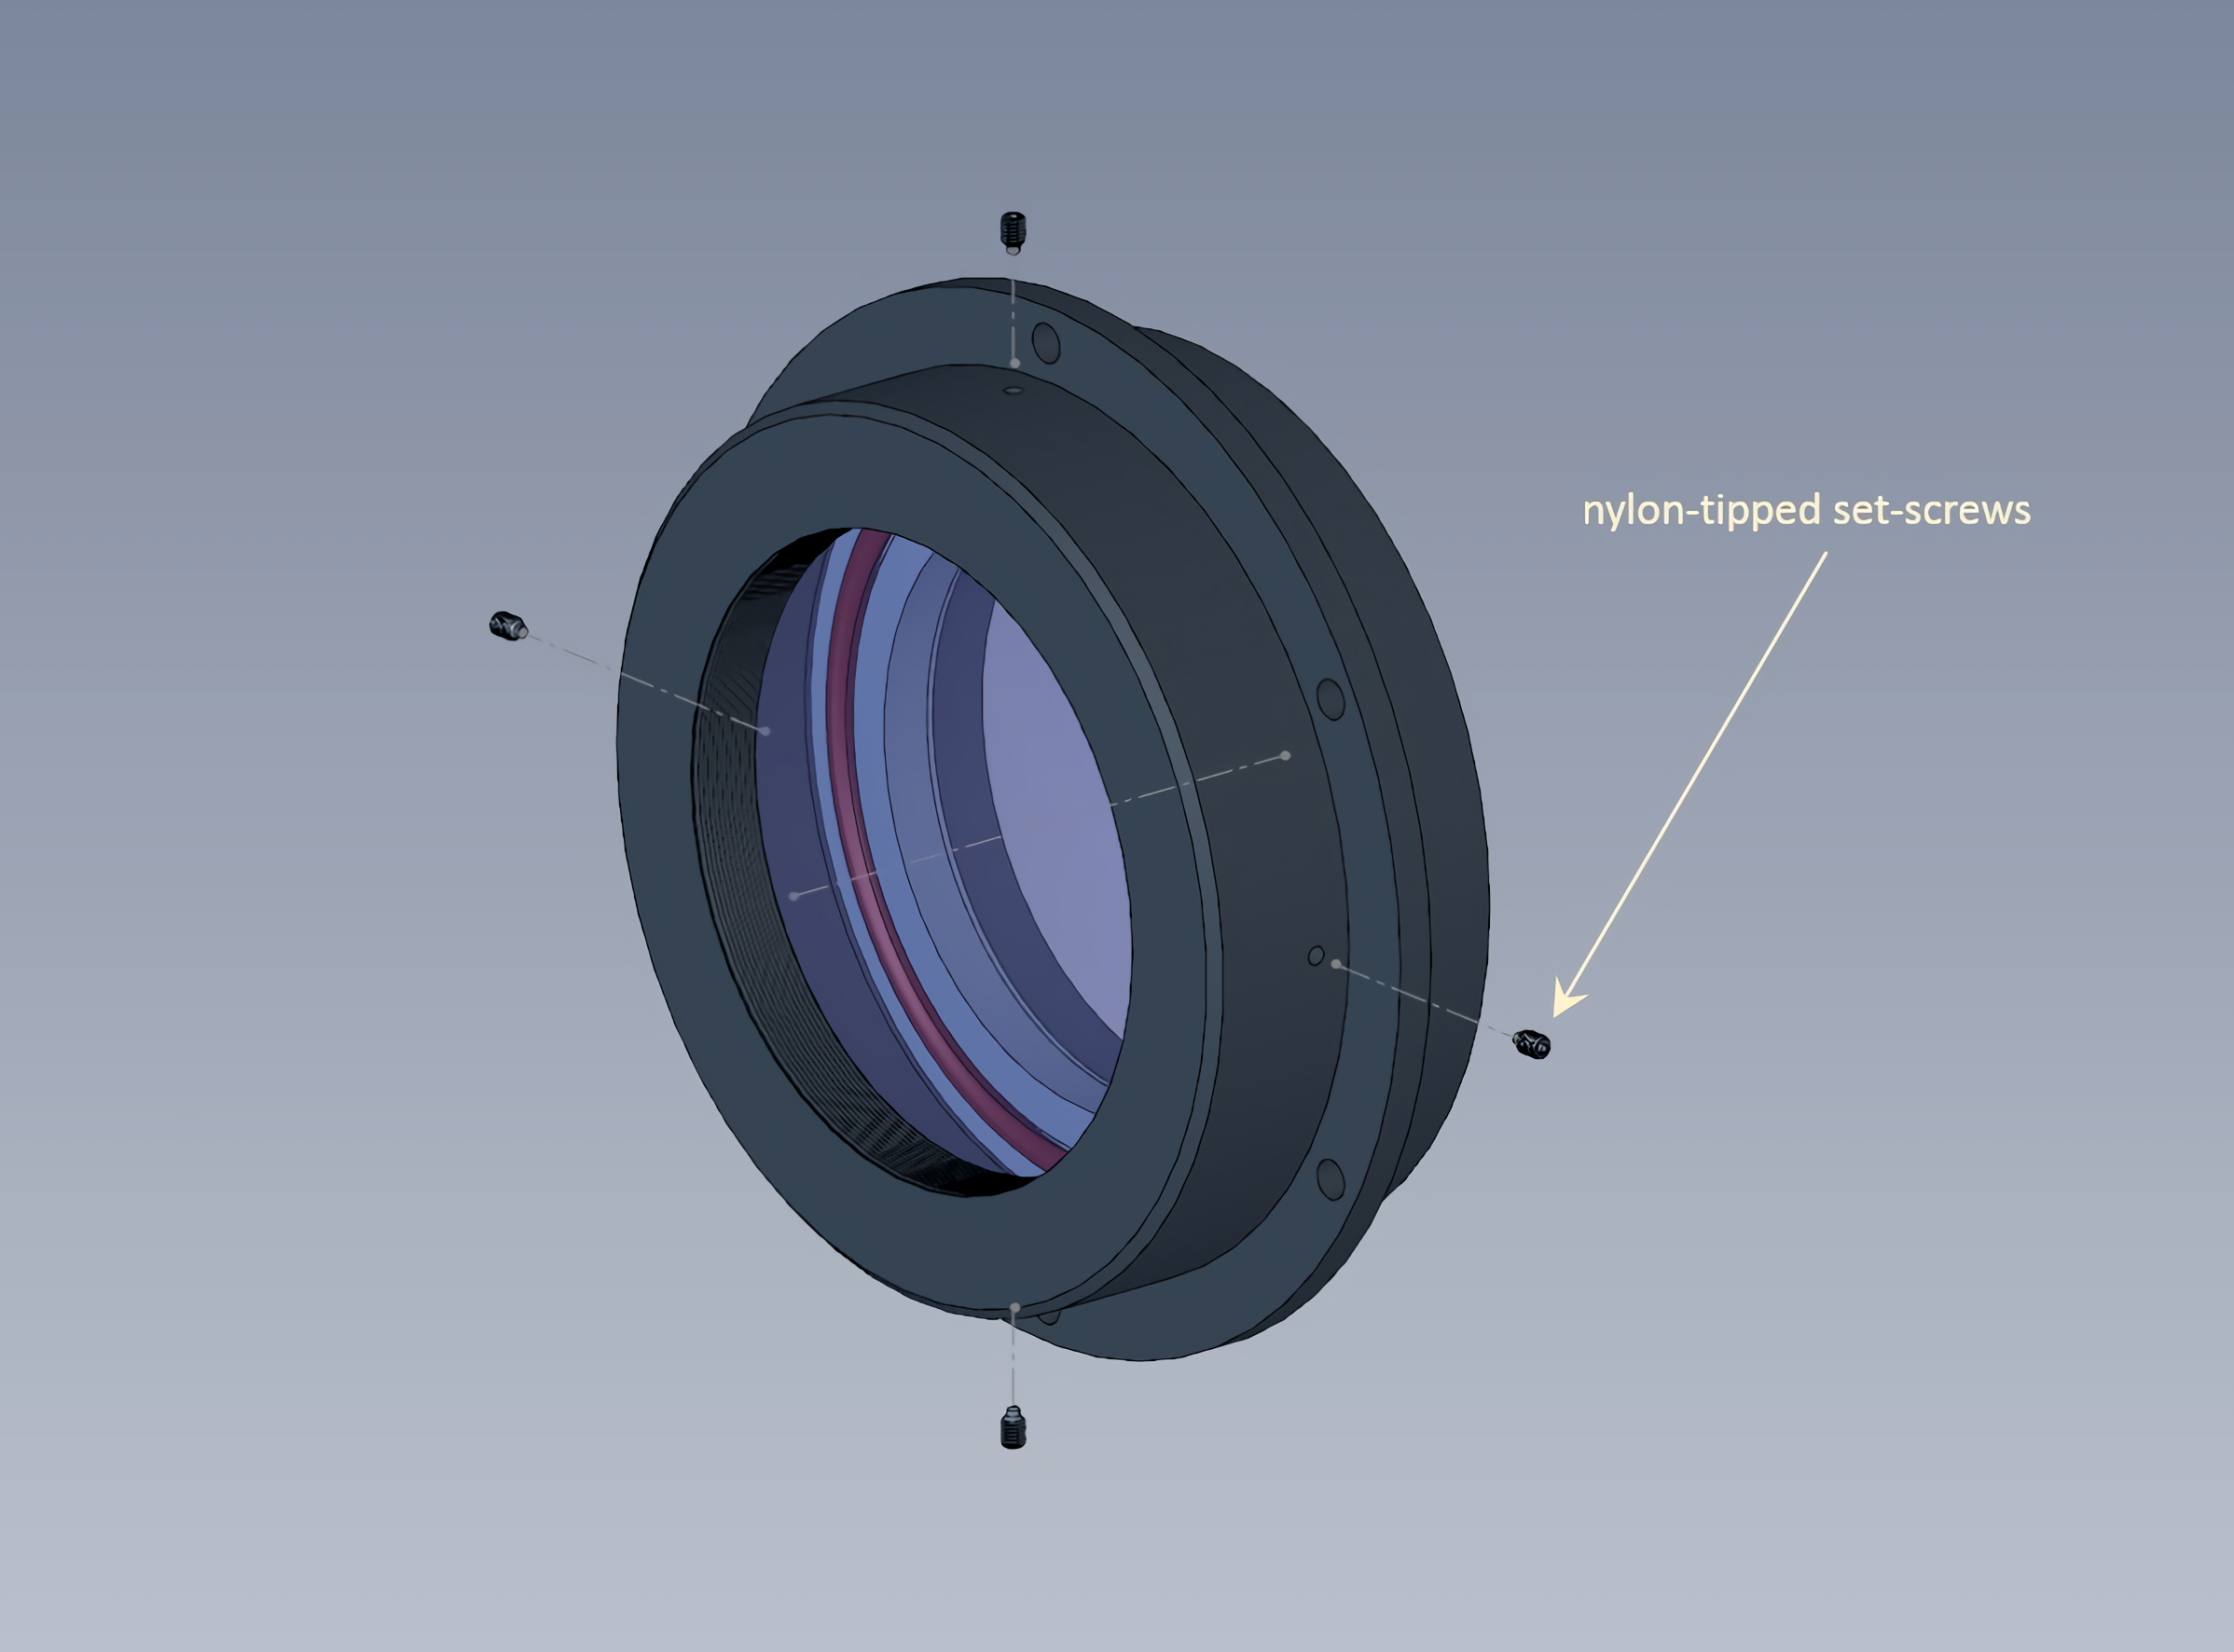
\includegraphics[width=0.7\linewidth]{figures/rosalia-set-screws.png}
\end{center}
\caption{Set-Screws for Centering.}
\label{figure:rosalia-set-screws}
\end{figure}

Set-screws will be used to center the lenses and, for the L1+L2 doublet, the spacer (see Figure~\ref{figure:rosalia-set-screws}). These screws are 18-8 stainless steel nylon-tipped set screw M3$ \times 0.5$ with a length of 4 mm (McMaster part 90666A124)

An axial preload force will be applied to hold the lenses in their proper positions. 

\begin{figure}
\begin{center}
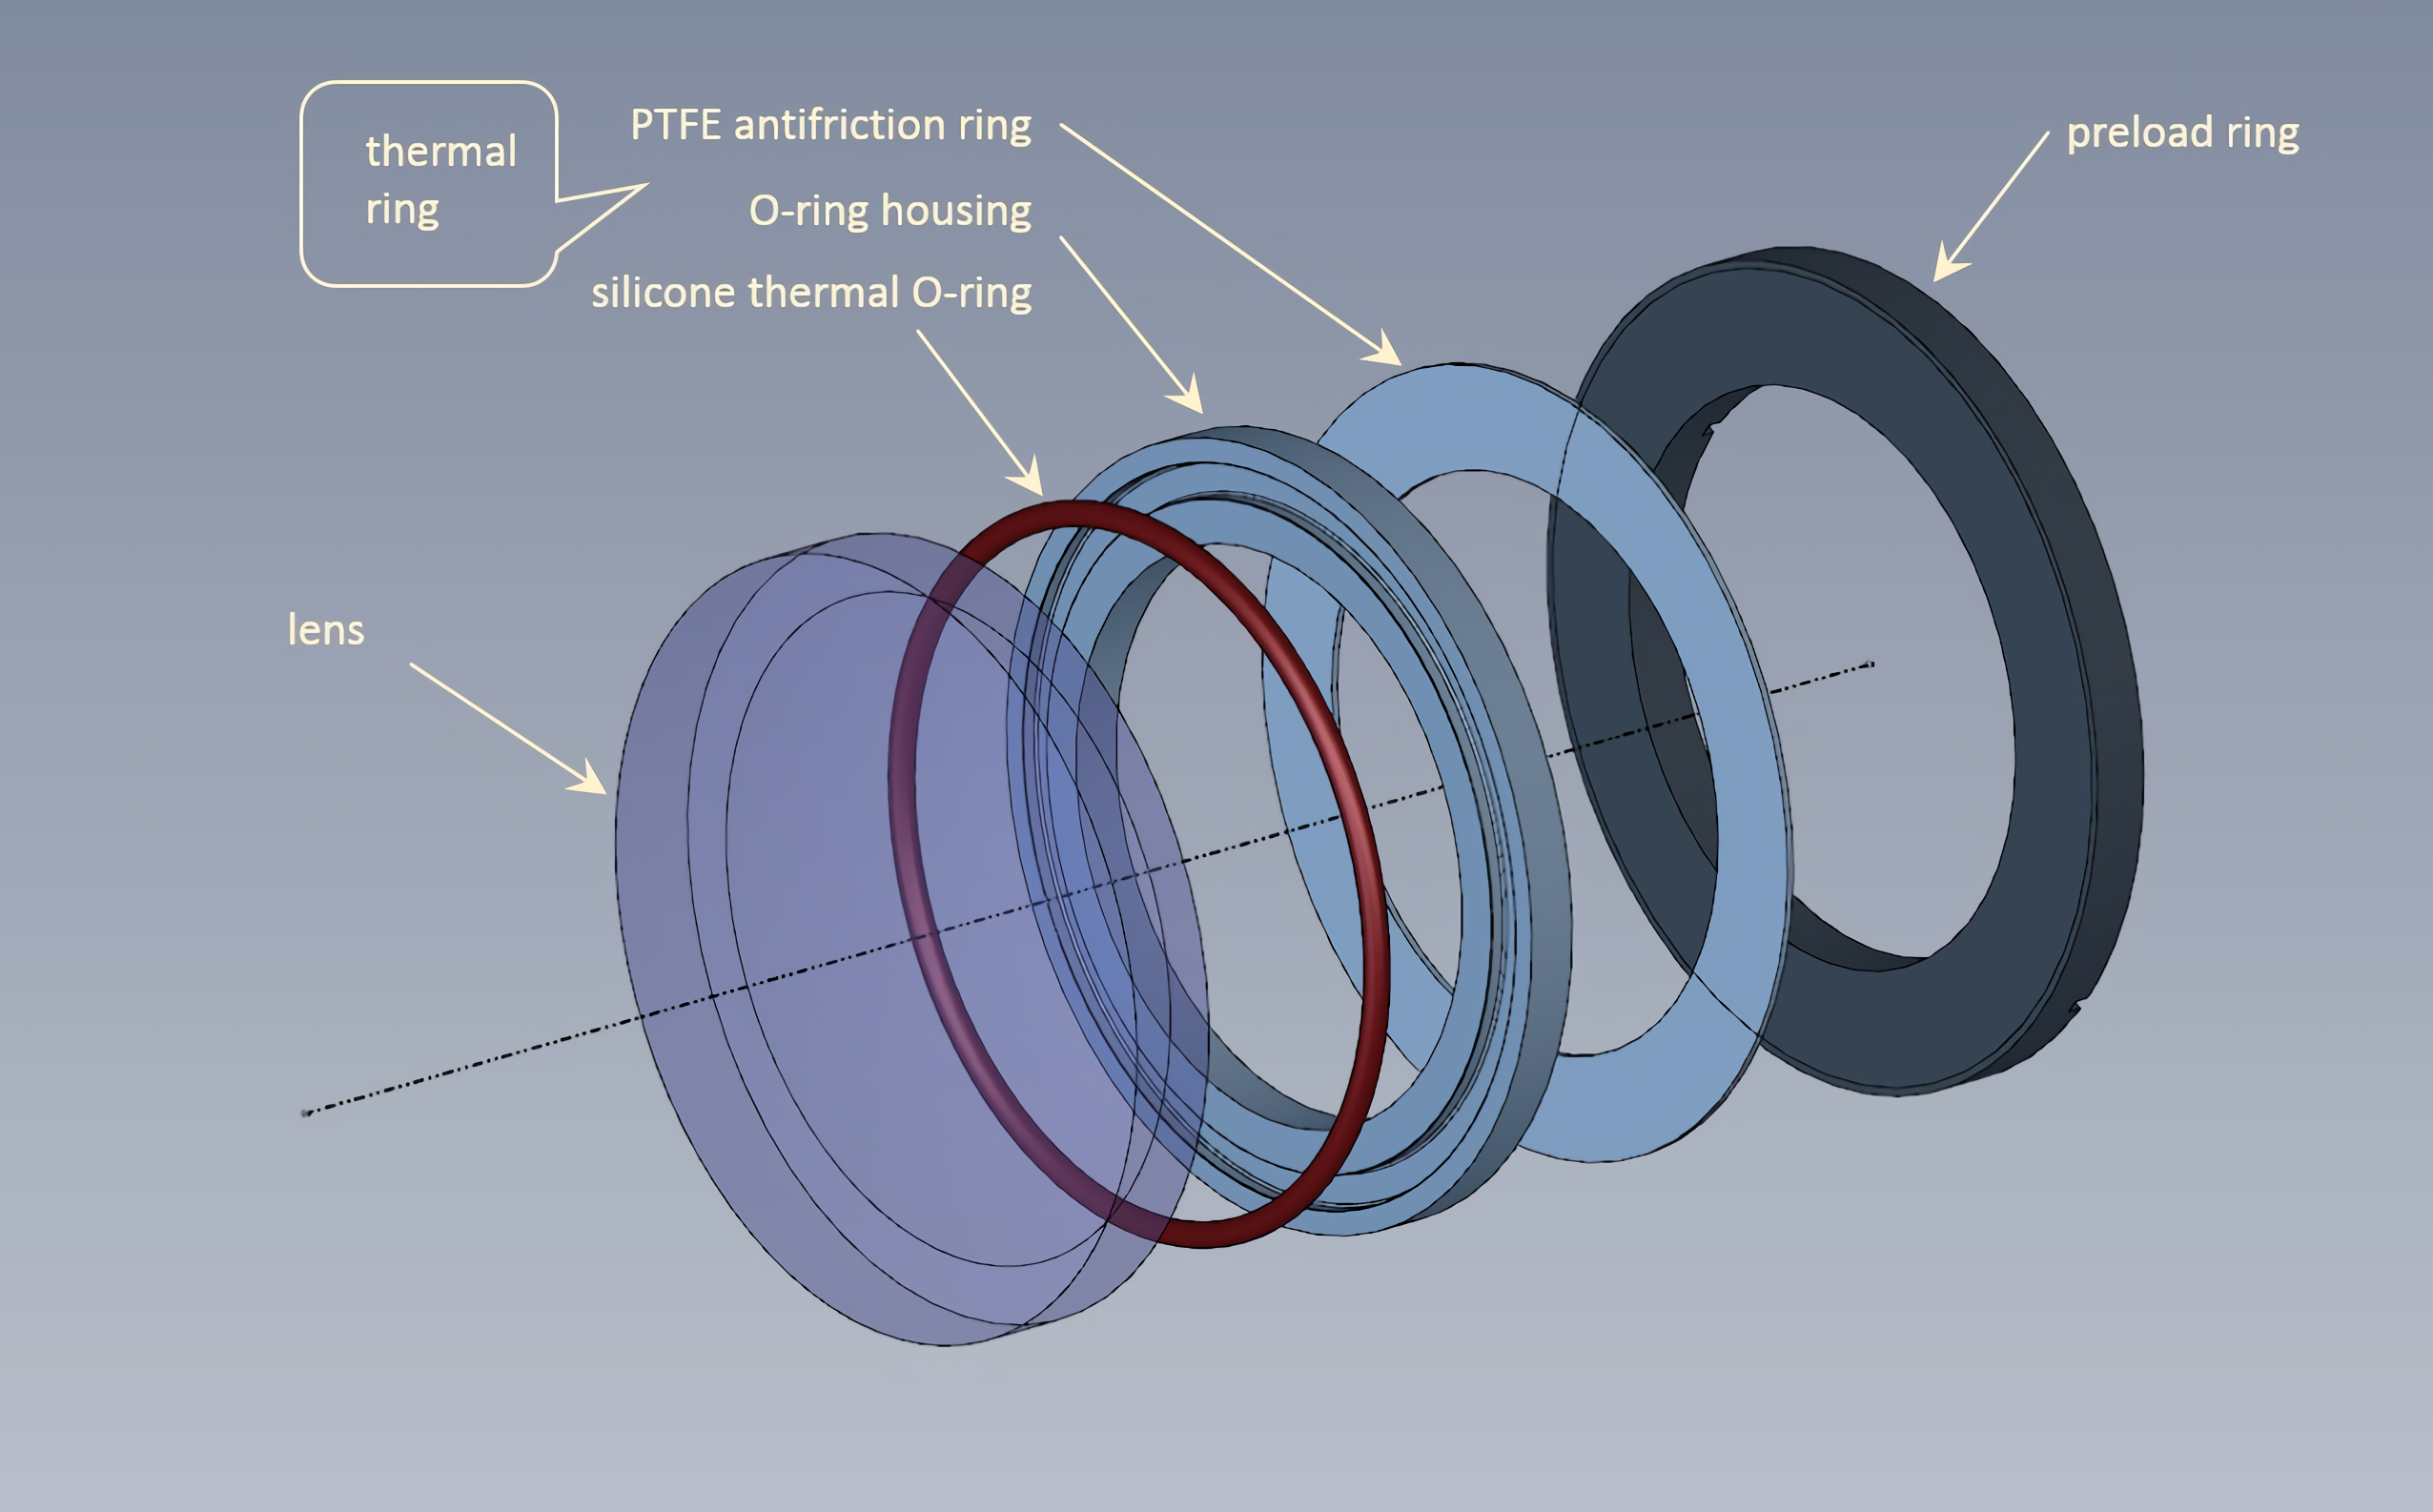
\includegraphics[width=0.7\linewidth]{figures/rosalia-rings.png}
\end{center}
\caption{The Preload Mechanism.}
\label{figure:rosalia-rings}
\end{figure}

This preload is applied -- and compensated thermally -- by four mechanical components after the last lens in the barrel (L2 or L3) and which are shown schematically in Figure~\ref{figure:rosalia-rings}. First, there is a silicone O-ring that makes contact with a flat bevel ground into the concave surface of the last lens. Next, there is an aluminum O-ring holder to support the O-ring. Then there is a thin PTFE (Teflon) friction-reducing ring cut from 0.8~mm (actually 1/32 inch). The PTFE sheet will be glued to the O-ring holder with epoxy resin. Finally, there is a threaded aluminum preload ring.

The preload will inevitably induce stress in the lenses. To reduce this to an aceptable level, the force should be distributed over a suitably large area of the lenses. Therefore, for the convex surfaces of the lenses we use tangential interfaces rather than corner interfaces. Since the lenses are meniscus, their other surfaces are concave and we cannot directly use tangential interfaces. Instead, the lenses will have flat bevels ground into the circumference of their concave sides and we will use simple parallel interfaces with these.

Table~\ref{table:lens-barrel-product-tree} shows an extract of the product tree table relevant for the lens supports.

\begin{table}
\caption{Extract of the Product Tree Table Relevant for the Lens Mounts}
\label{table:lens-barrel-product-tree}
\begin{center}
\small
\begin{tabular}{ll}
\hline
\hline
Code                &Description\\
\hline
DR-ME-OML1L2        &Optomechanics for L1 and L2\\
DR-ME-OML1L2-BAR    &Barrel\\
DR-OP-L1            &Lens L1\\
DR-ME-OML1L2-SPA		&Spacer\\
DR-OP-L2            &Lens L2\\
DR-ME-OML1L2-OR		  &O-Ring (Silicone)\\
DR-ME-OML1L2-ORH		&O-Ring Holder\\
DR-ME-OML1L2-FRR		&Friction-Reducing Ring (PTFE)\\
DR-ME-OML1L2-PLR		&Preload Ring\\
DR-ME-OML1L2-CSS		&Centering Set-Screw\\
\hline
DR-ME-OML3          &Optomechanics for L3\\
DR-ME-OM3-LBR       &L-Bracket\\
DR-ME-OM3-BAR       &Barrel\\
DR-OP-L3            &Lens L3\\
DR-ME-OML3-OR		    &O-Ring (Silicone)\\
DR-ME-OML3-ORH	  	&O-Ring Holder\\
DR-ME-OML3-FRR	  	&Friction-Reducing Ring (PTFE)\\
DR-ME-OML3-PLR	  	&Preload Ring\\
DR-ME-OML3-CSS	  	&Centering Set-Screw\\
%\hline
%DR-ME-OML4          &Optomechanics for L4\\
%DR-ME-OM4-LBR       &L-Bracket\\
%DR-ME-OM4-BAR       &Barrel\\
%DR-OP-L4            &Lens L4\\
%DR-ME-OML4-OR	   	  &O-Ring (Silicone)\\
%DR-ME-OML4-ORH  		&O-Ring Holder\\
%DR-ME-OML4-FRR  		&Friction-Reducing Ring (PTFE)\\
%DR-ME-OML4-PLR  		&Preload Ring\\
%DR-ME-OML4-CSS	  	&Centering Set-Screw\\
\hline
\end{tabular}
\end{center}
\end{table}

Table~\ref{table:physical-properties} gives the physical properties of the materials used: the thermal expansion coefficient $\alpha$, the Poisson ratio $\nu$, the modulus of elasticity $E$, and density $\rho$.

\begin{table}
\caption{Physical Properties of Materials}
\label{table:physical-properties}
\begin{center}
\small
\begin{tabular}{lccccl}
\hline
\hline
Material&
$\alpha$&
$\nu$&
$E$&
$\rho$&
Reference\\
&
\unit{C^{-1}}&
&
Pa&
\unit{g\,cm^{-3}}&
\\
\hline
\CaF&
$1.885 \times 10^{-5}$&
0.26&
$7.580 \times 10^{10}$&
3.18\phantom{0}&
oharacorp.com\\
N-BaK4&
$7.000 \times 10^{-6}$&
0.24&
$7.700 \times 10^{10}$&
3.05\phantom{0}&
schott.com\\
Fused Silica&
$5.000 \times 10^{-7}$&
0.16&
$7.270 \times 10^{10}$&
2.201&
corning.com\\
Aluminium 7050&
$2.37\phantom{0} \times 10^{-5}$&
0.33&
$7.20\phantom{0} \times 10^{10}$&
2.82\phantom{0}&
carrs-tool.co.uk\\
Silicone (50 durometer)&
$1.80\phantom{0} \times 10^{-4}$&
0.5\phantom{0}&
$8.5\phantom{00} \times 10^{5\phantom{0}}$&
1.1\phantom{00}&
parker.com\\
Silicone (70 durometer)&
$2.30\phantom{0} \times 10^{-4}$&
0.5\phantom{0}&
$4.14\phantom{0} \times 10^{6\phantom{0}}$&
1.1\phantom{00}&
parker.com\\
PTFE&
$8.00\phantom{0} \times 10^{-5}$&
0.46&
$5.17\phantom{0} \times 10^{8\phantom{0}}$&
2.18\phantom{0}&
elaplas.es\\
\hline
\end{tabular}
\end{center}
\end{table}

\begin{figure}
\begin{center}
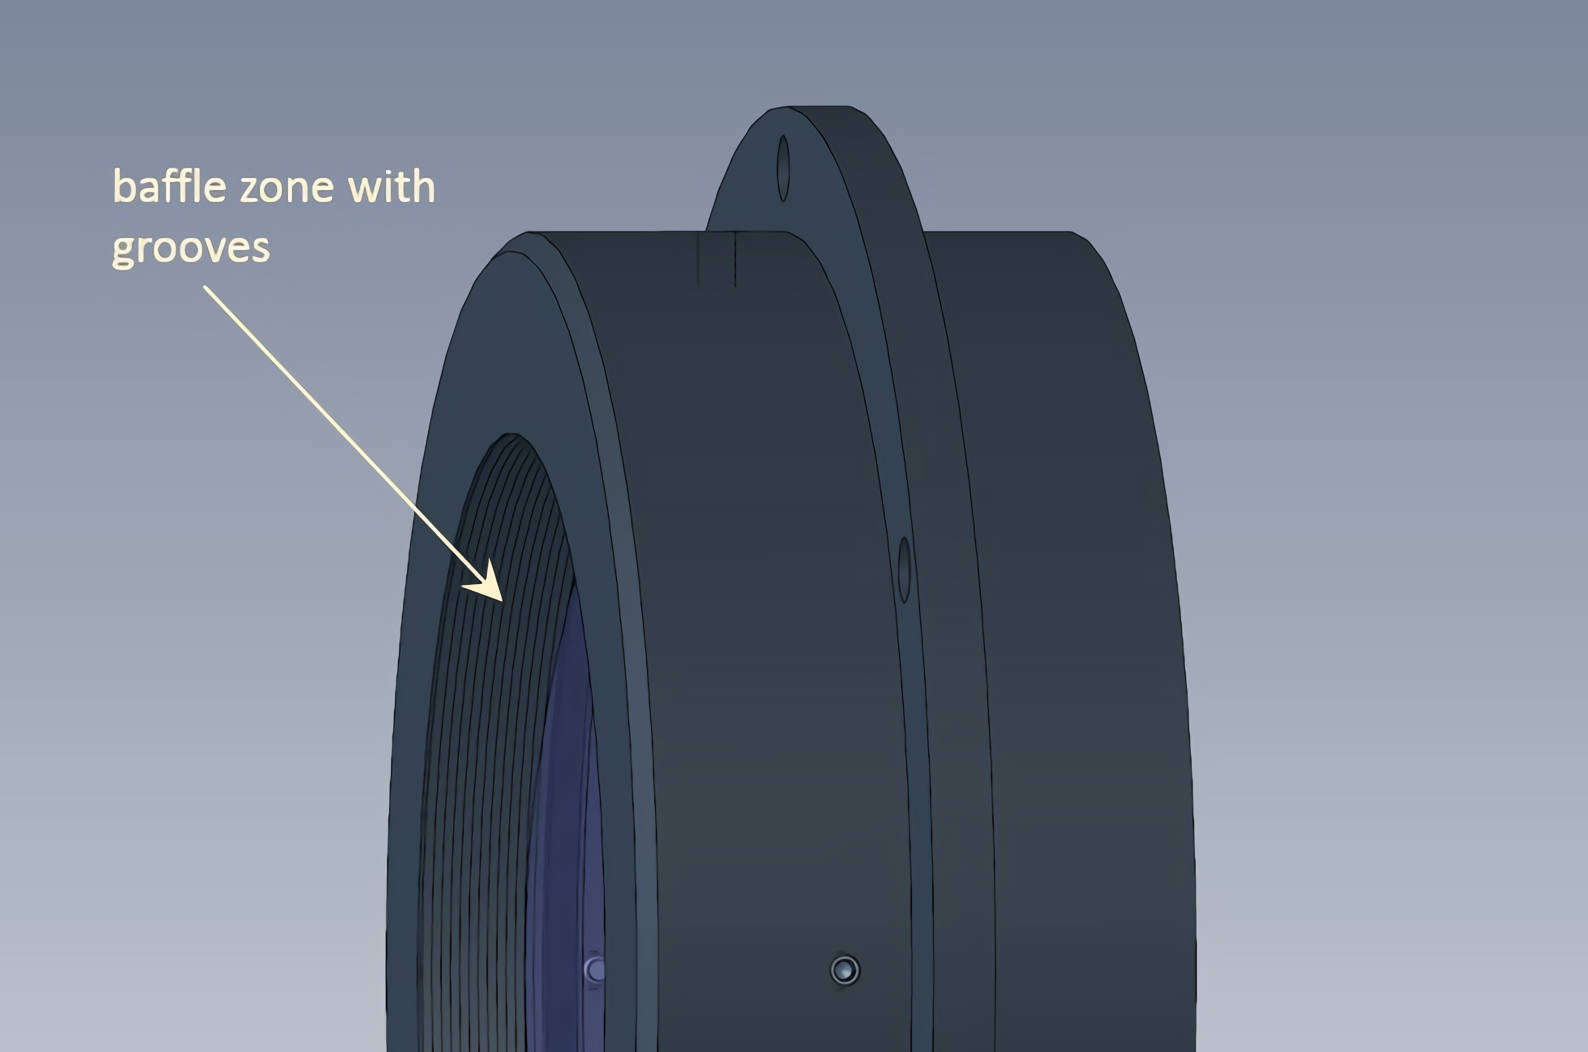
\includegraphics[width=0.7\linewidth]{figures/rosalia-grooves.png}
\end{center}
\caption{Grooves to Reduce Scattered Light.}
\label{figure:rosalia-grooves}
\end{figure}

The inner diameter at the entrance of each barrel will have an appropriate dimension so to act as a baffle. Furthermore, the inner surfaces of the barrel and aluminum rings will be grooved with a pattern of sharp ridges 800~{\micron} deep and with a spacing of 1000~{\micron} between peaks (see Figure~\ref{figure:rosalia-grooves}).

\subsubsection{The DR-ME-OML1L2 Mount for L1+L2}

\begin{figure}
\begin{center}
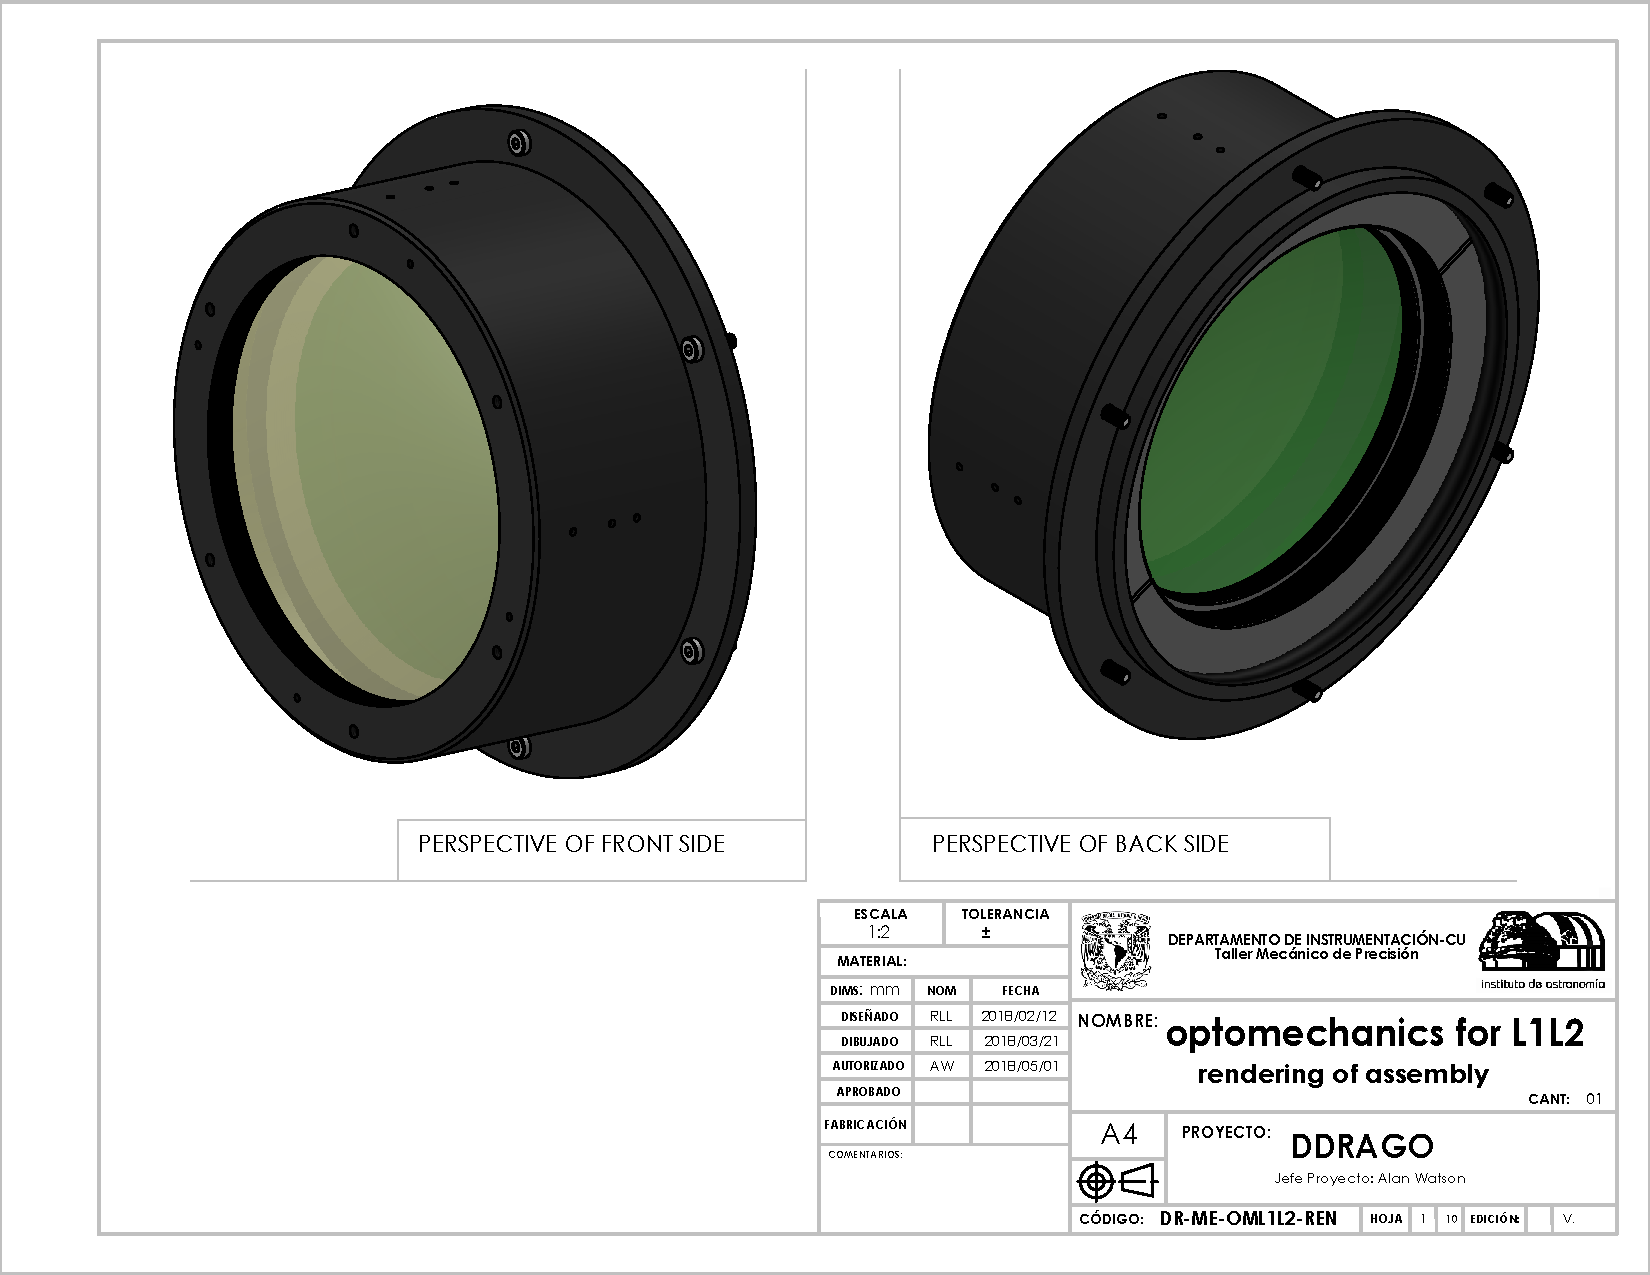
\includegraphics[height=\linewidth,angle=90]{figures/DR-ME-OML1L2-REN}
\end{center}
\caption{The DR-ME-OML1L2 Barrel for L1 and L2: Perspective}
\label{figure:rosalia-oml1l2-perspective}
\end{figure}

\begin{figure}
\begin{center}
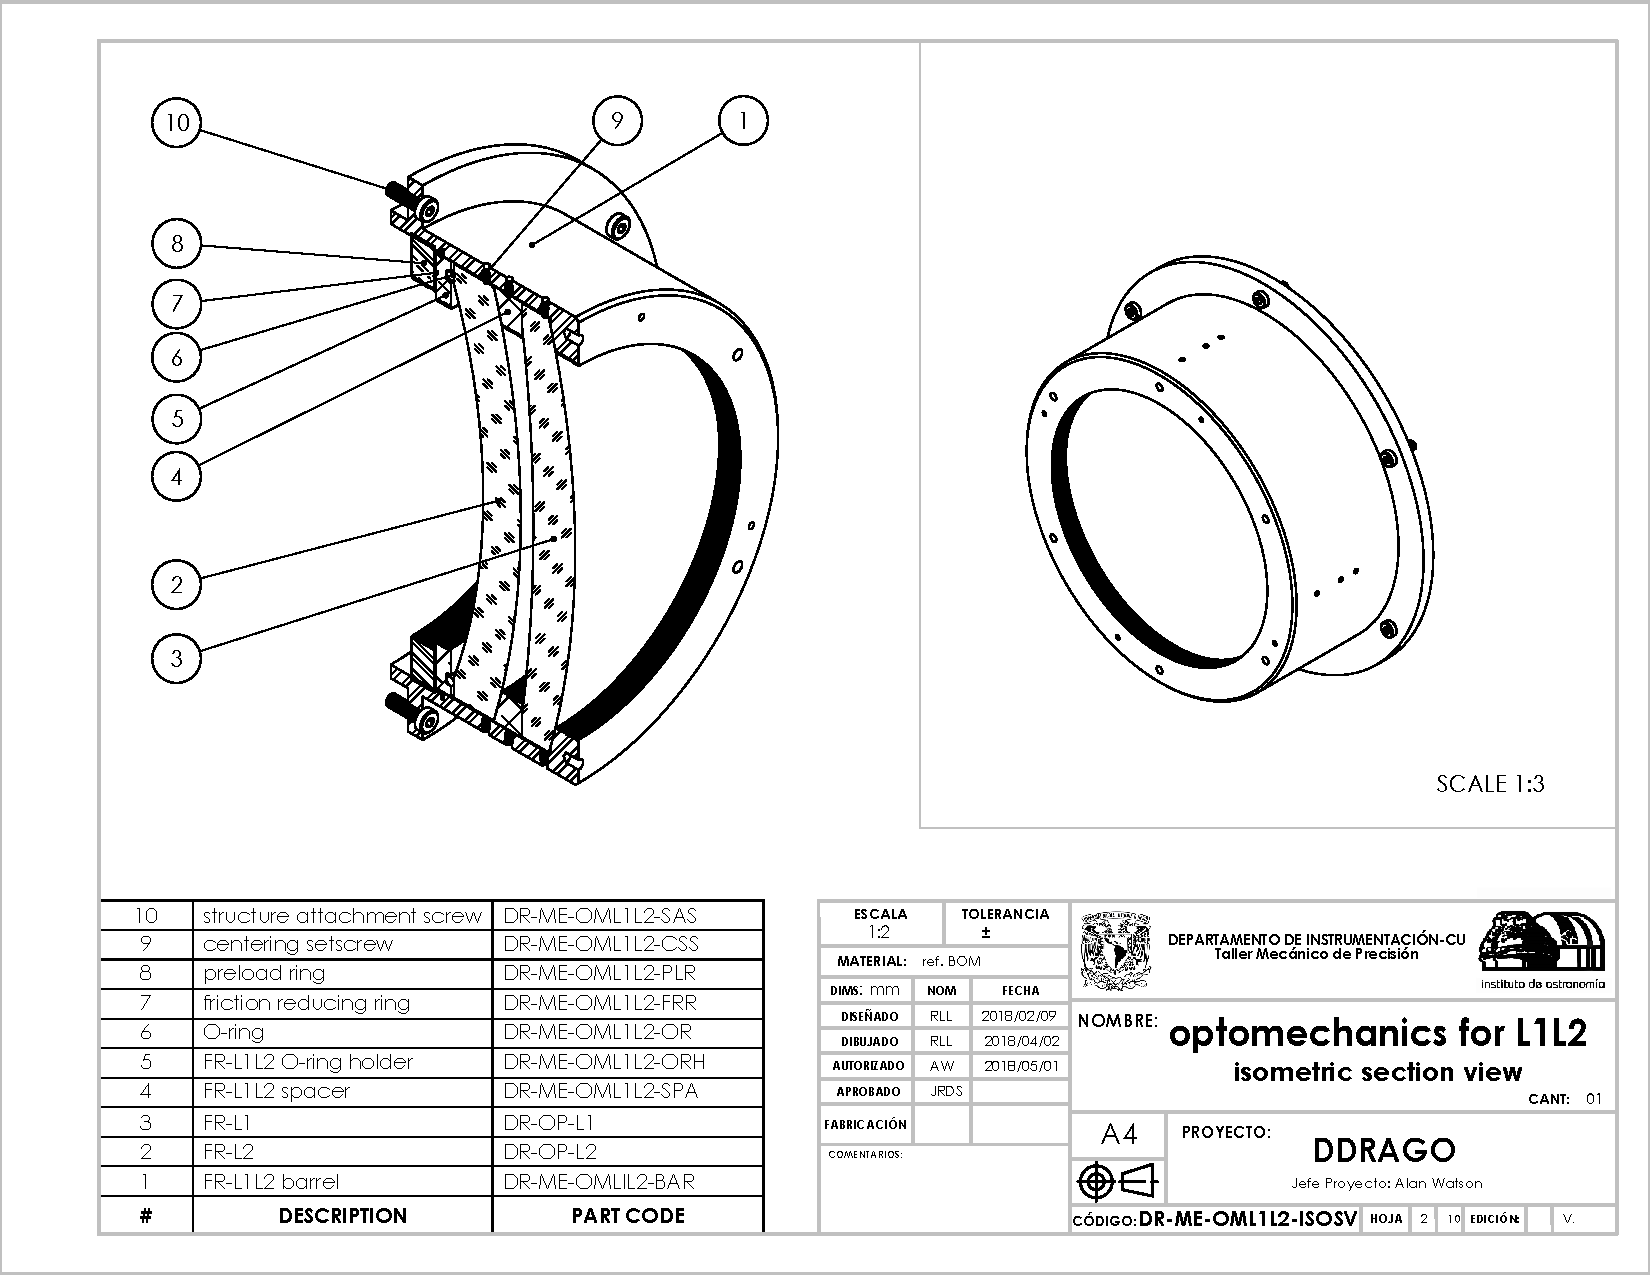
\includegraphics[height=\linewidth,angle=90]{figures/DR-ME-OML1L2-ISOSV}
\end{center}
\caption{The DR-ME-OML1L2 Barrel for L1 and L2: Section View}
\label{figure:rosalia-oml1l2-section}
\end{figure}

\begin{figure}
\begin{center}
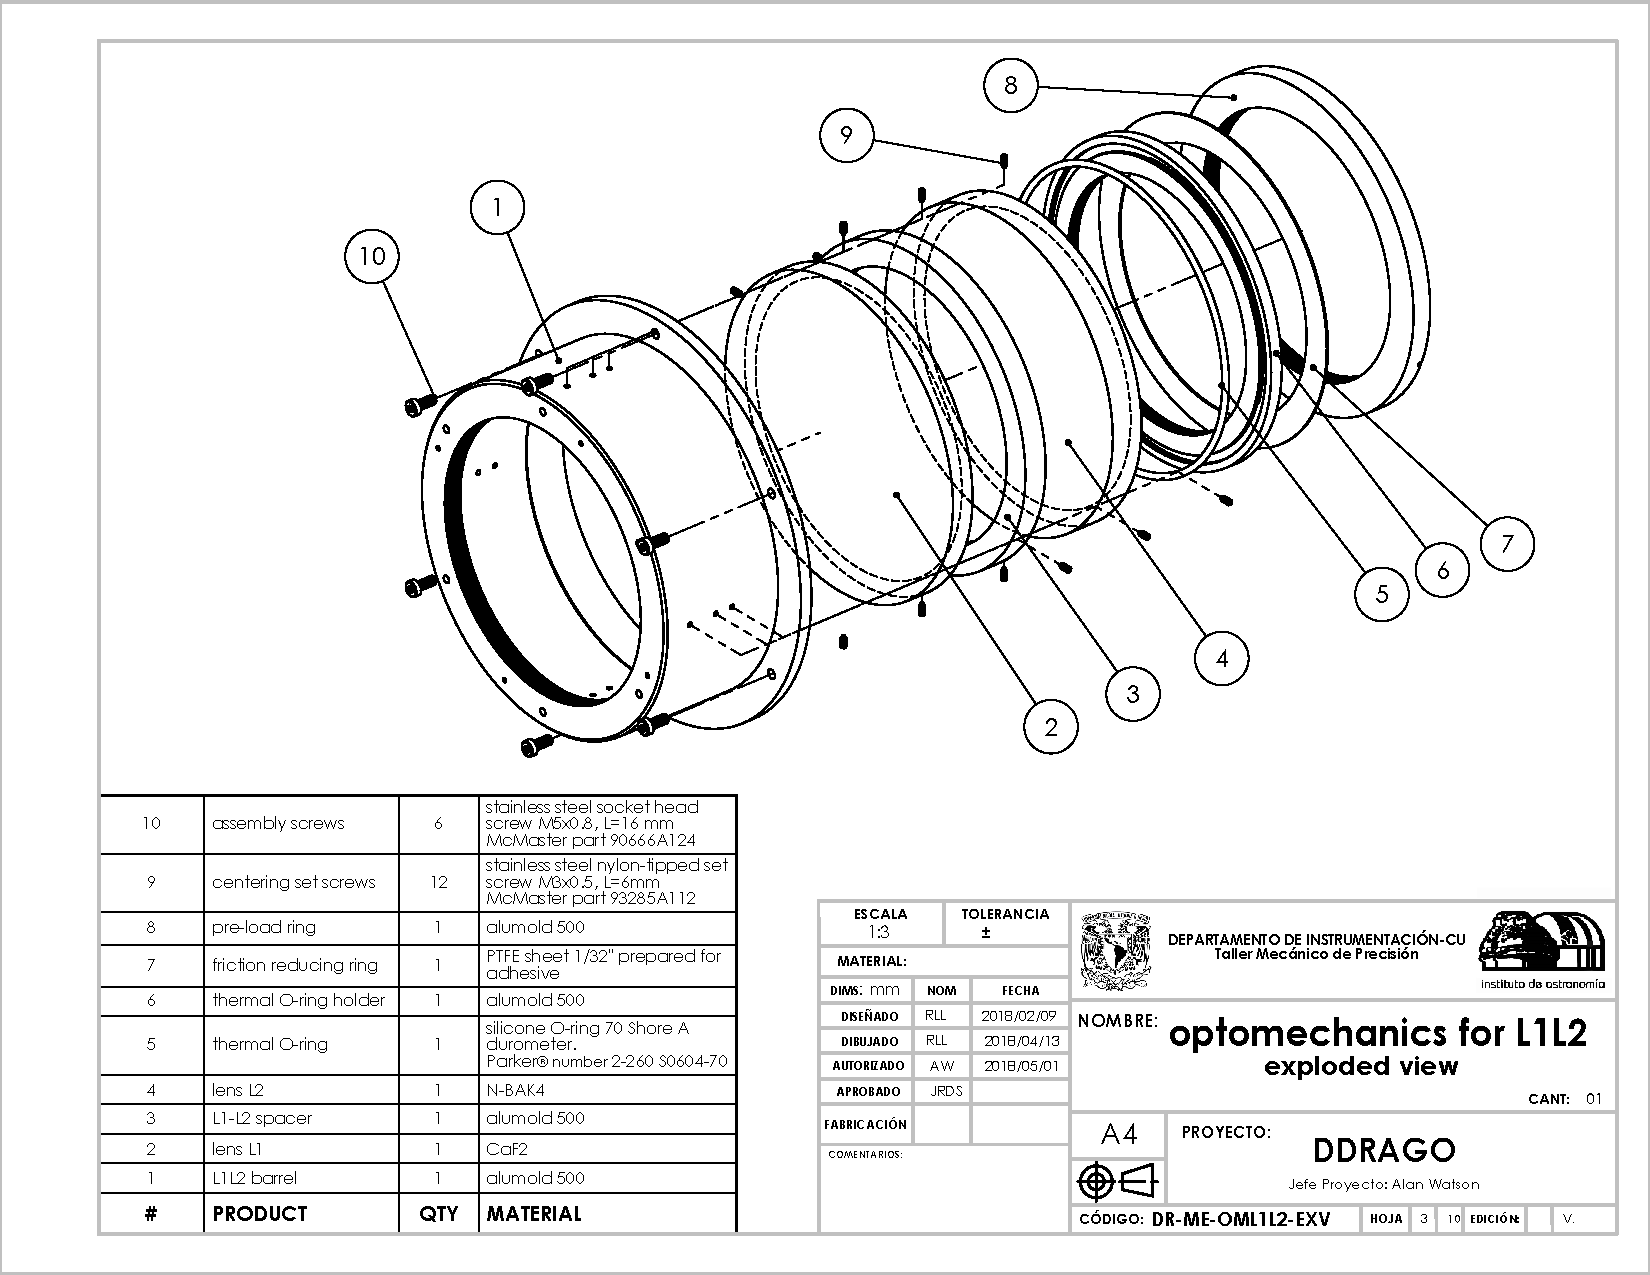
\includegraphics[height=\linewidth,angle=90]{figures/DR-ME-OML1L2-EXV}
\end{center}
\caption{The DR-ME-OML1L2 Barrel for L1 and L2: Exploded View}
\label{figure:rosalia-oml1l2-exploded}
\end{figure}

\begin{figure}
\begin{center}
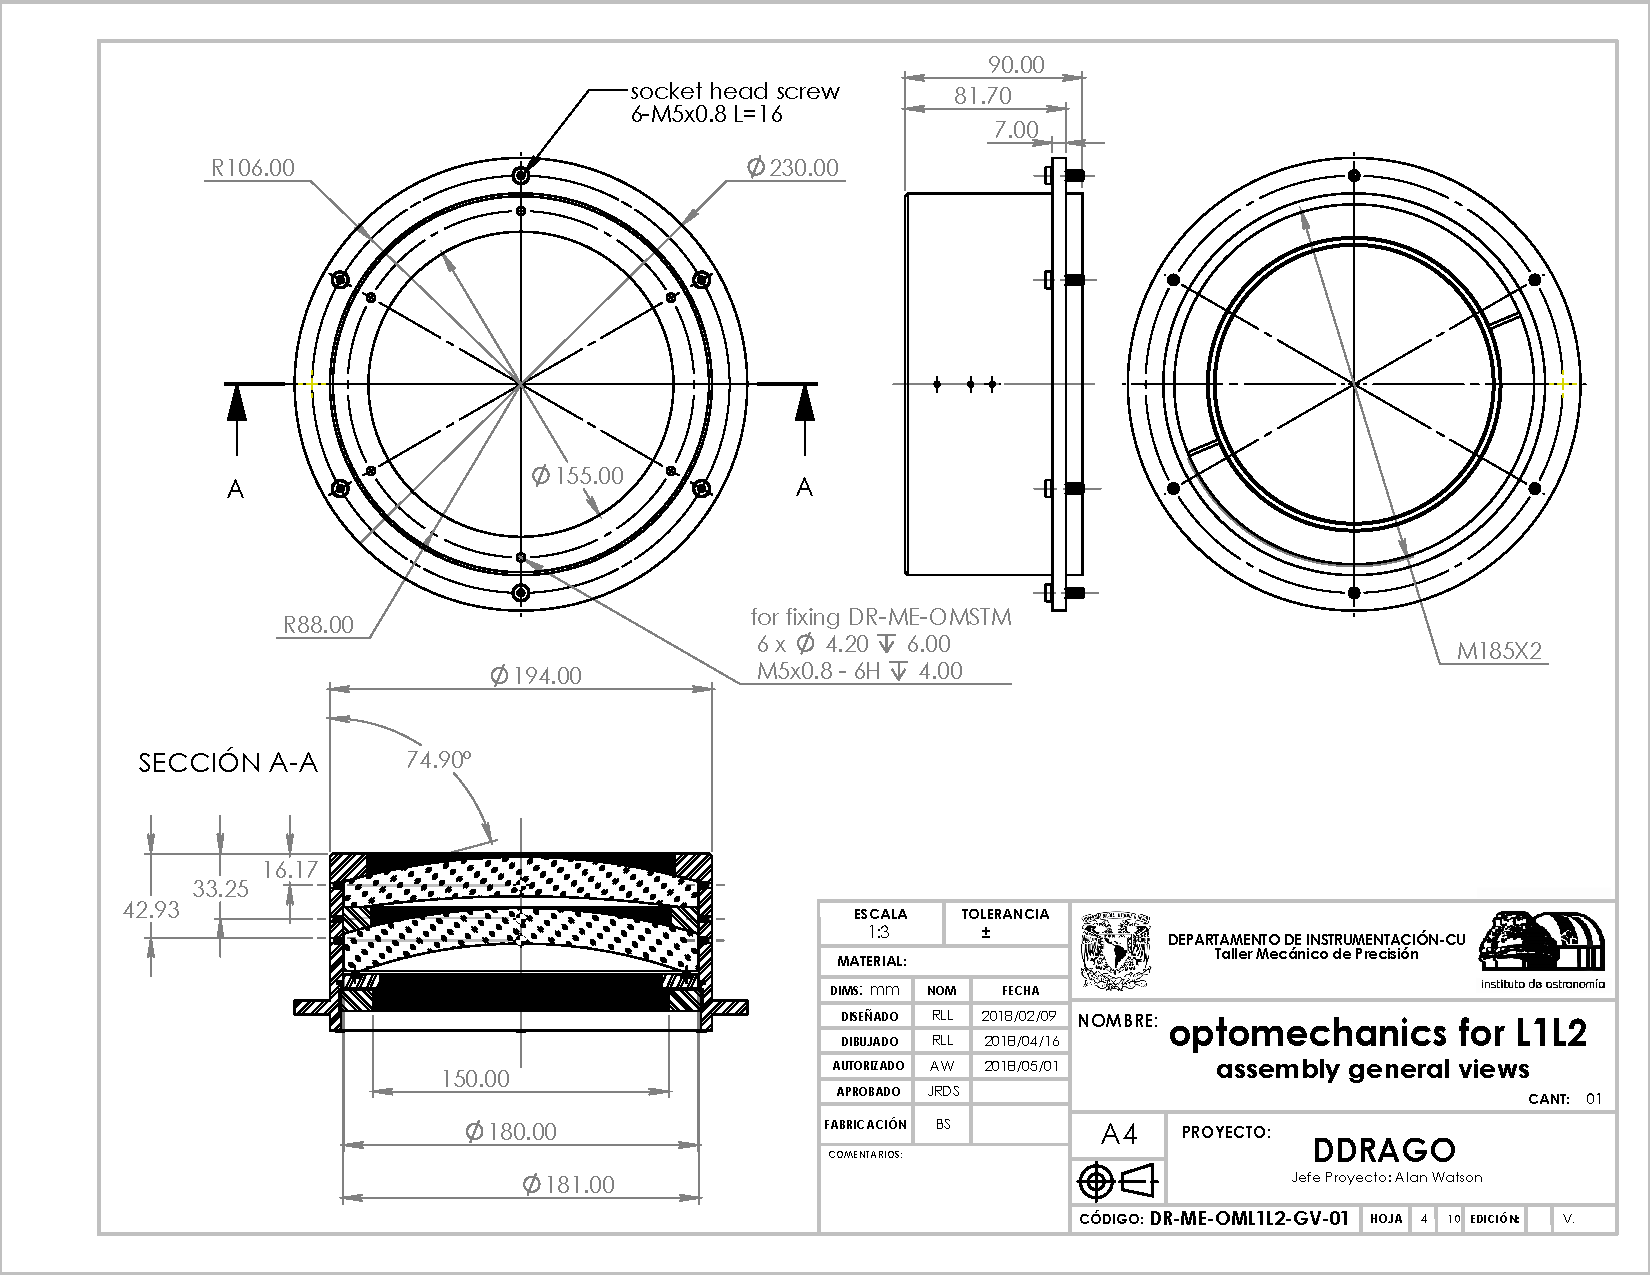
\includegraphics[height=\linewidth,angle=90]{figures/DR-ME-OML1L2-GV-01}
\end{center}
\caption{The DR-ME-OML1L2 Barrel for L1 and L2: General View}
\label{figure:rosalia-oml1l2-general}
\end{figure}

\begin{figure}
\begin{center}
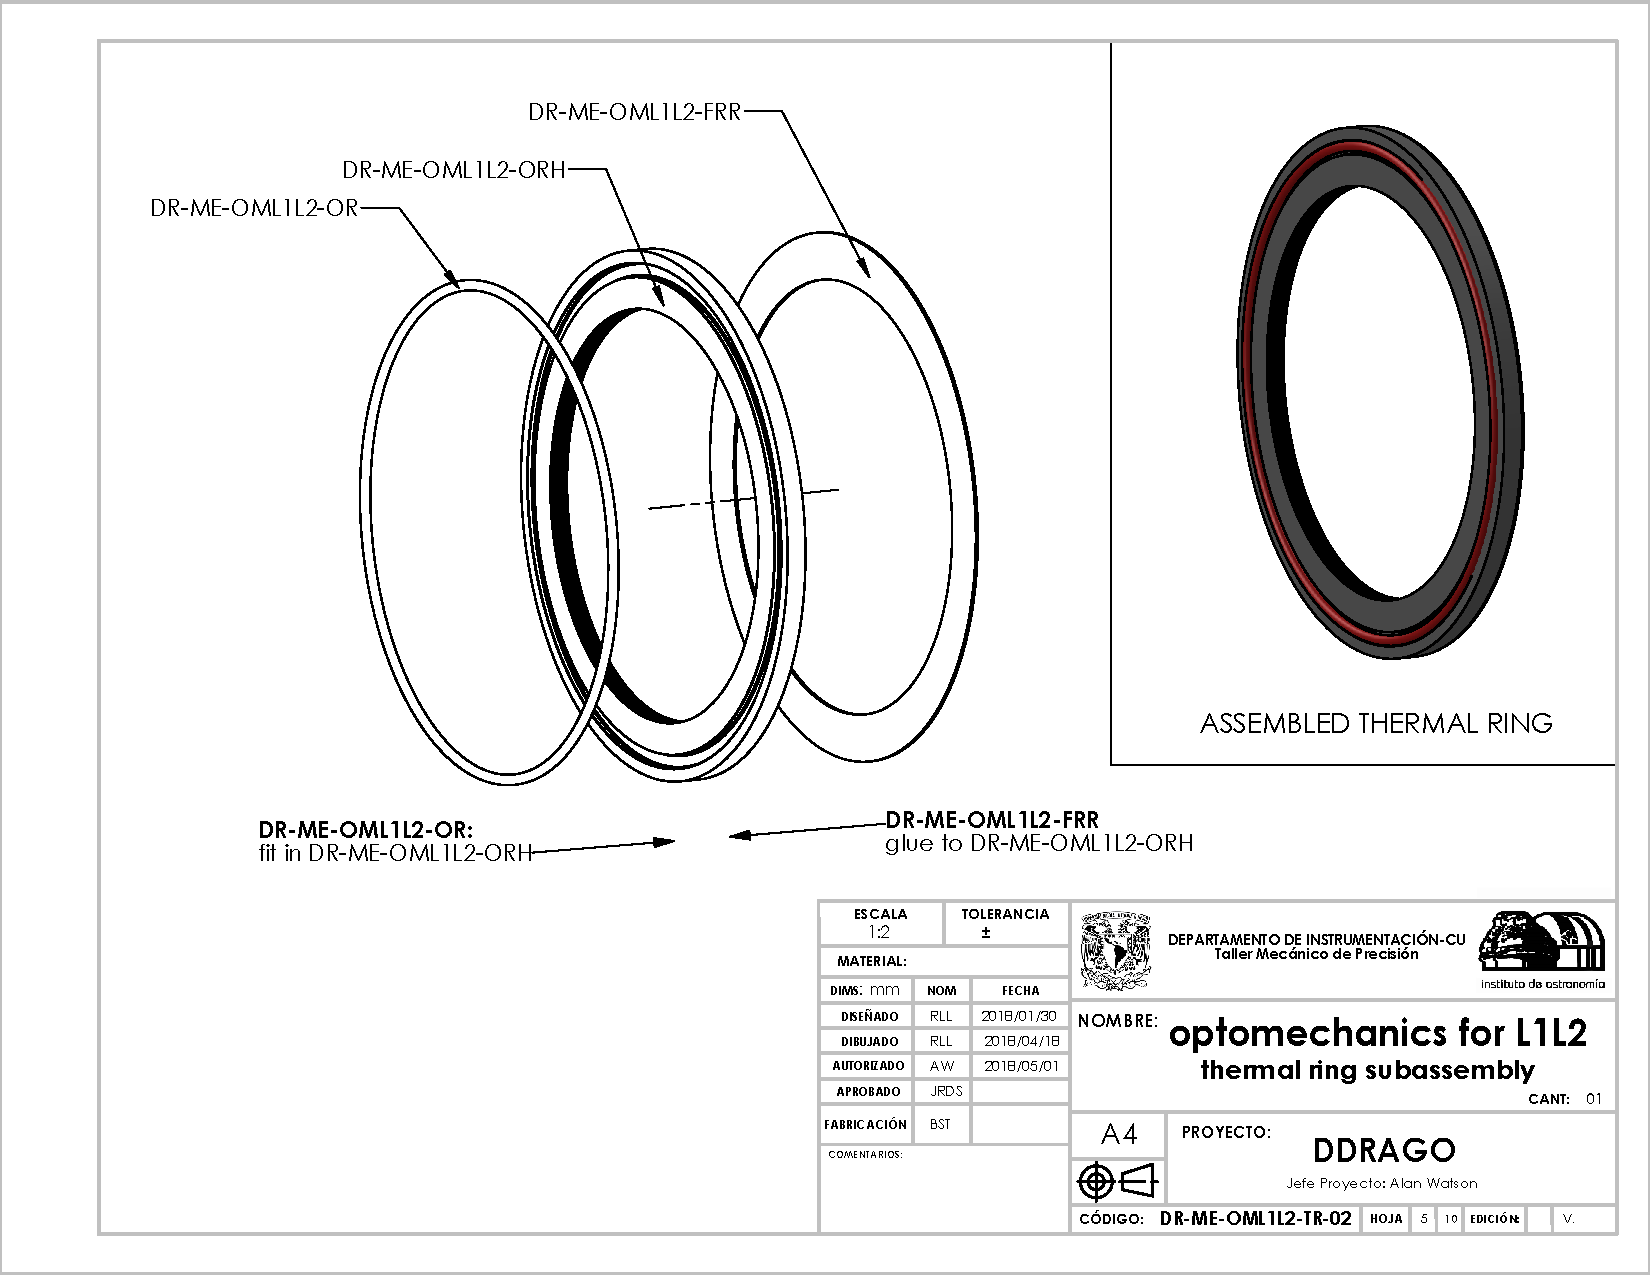
\includegraphics[height=\linewidth,angle=90]{figures/DR-ME-OML1L2-TR-02}
\end{center}
\caption{The DR-ME-OML1L2 Barrel for L1 and L2: The DR-ME-OML1L2-TR Thermal Ring Assembly}
\label{figure:rosalia-oml1l2-thermal-ring}
\end{figure}

\begin{figure}
\begin{center}
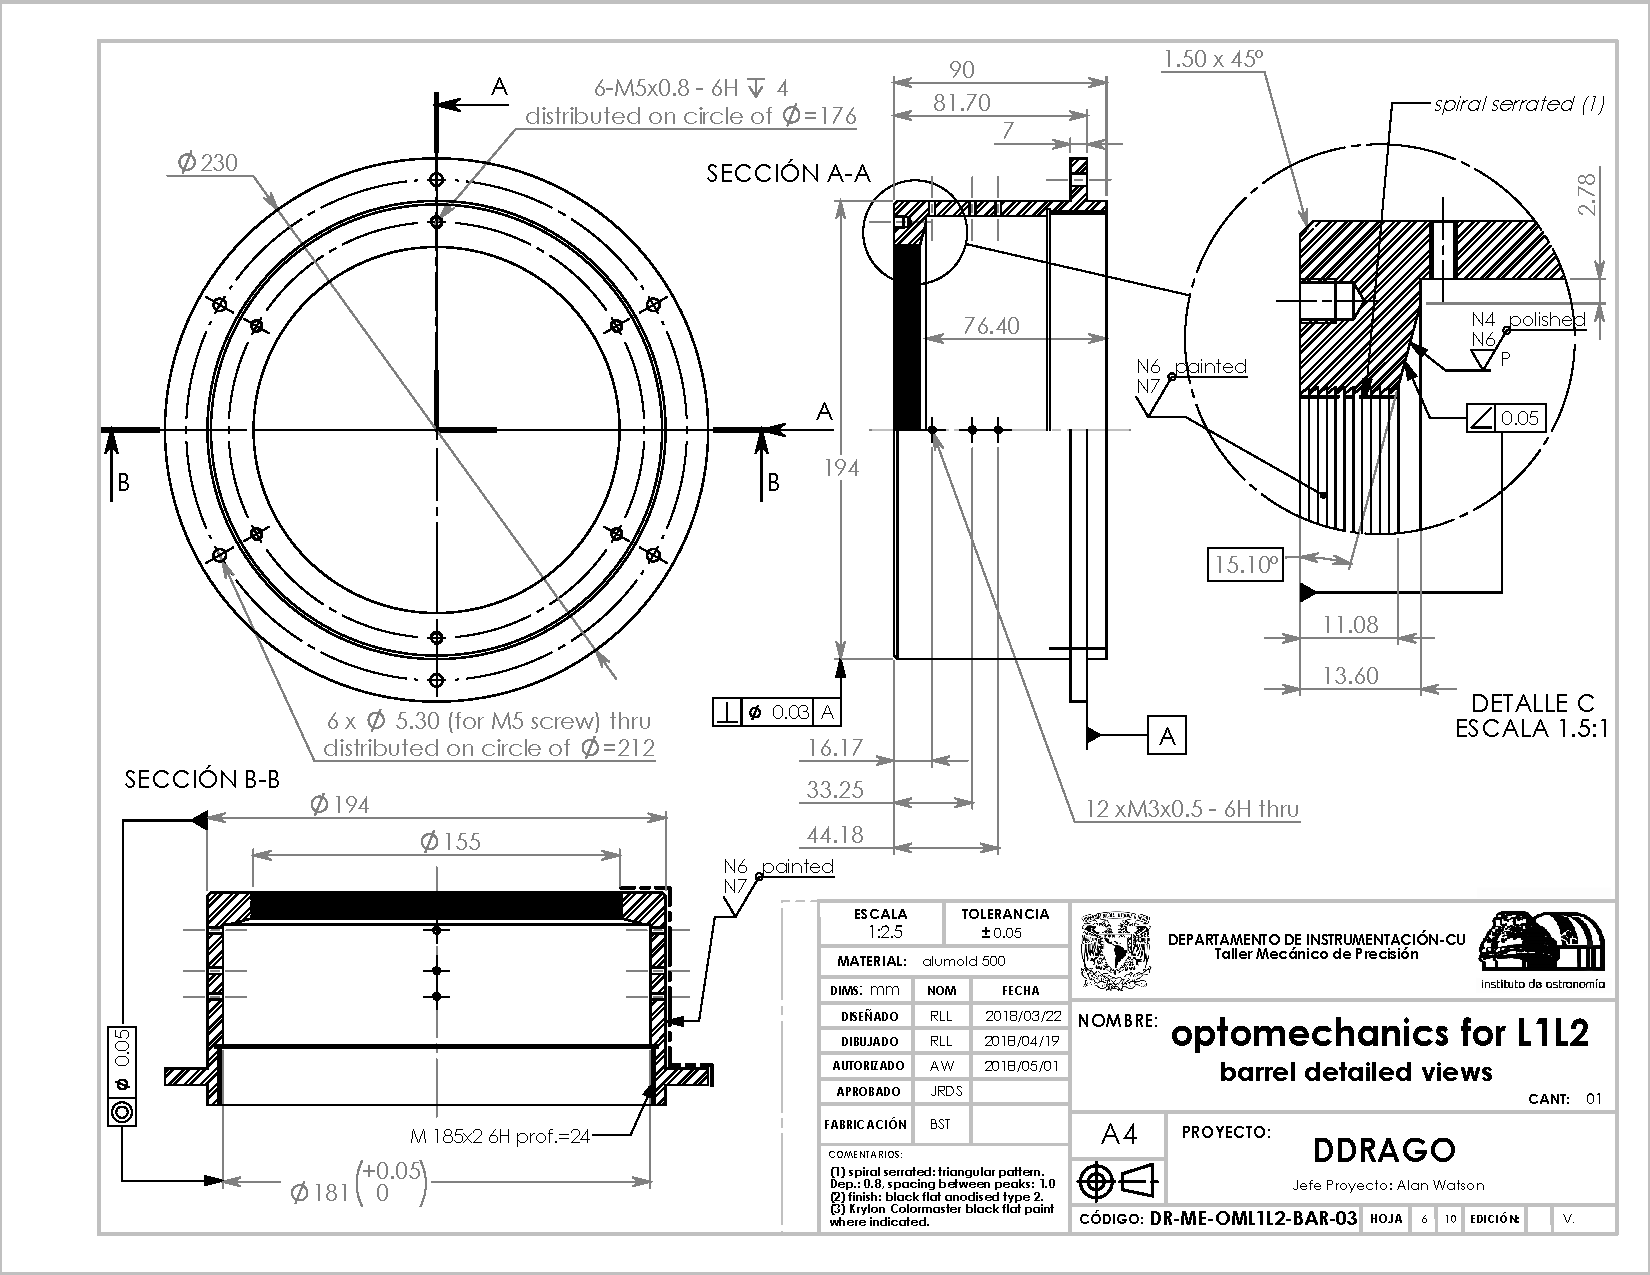
\includegraphics[height=\linewidth,angle=90]{figures/DR-ME-OML1L2-BAR-03}
\end{center}
\caption{The DR-ME-OML1L2 Barrel for L1 and L2: The DR-ME-OML1L2-BAR Barrel}
\label{figure:rosalia-oml1l2-bar}
\end{figure}

\begin{figure}
\begin{center}
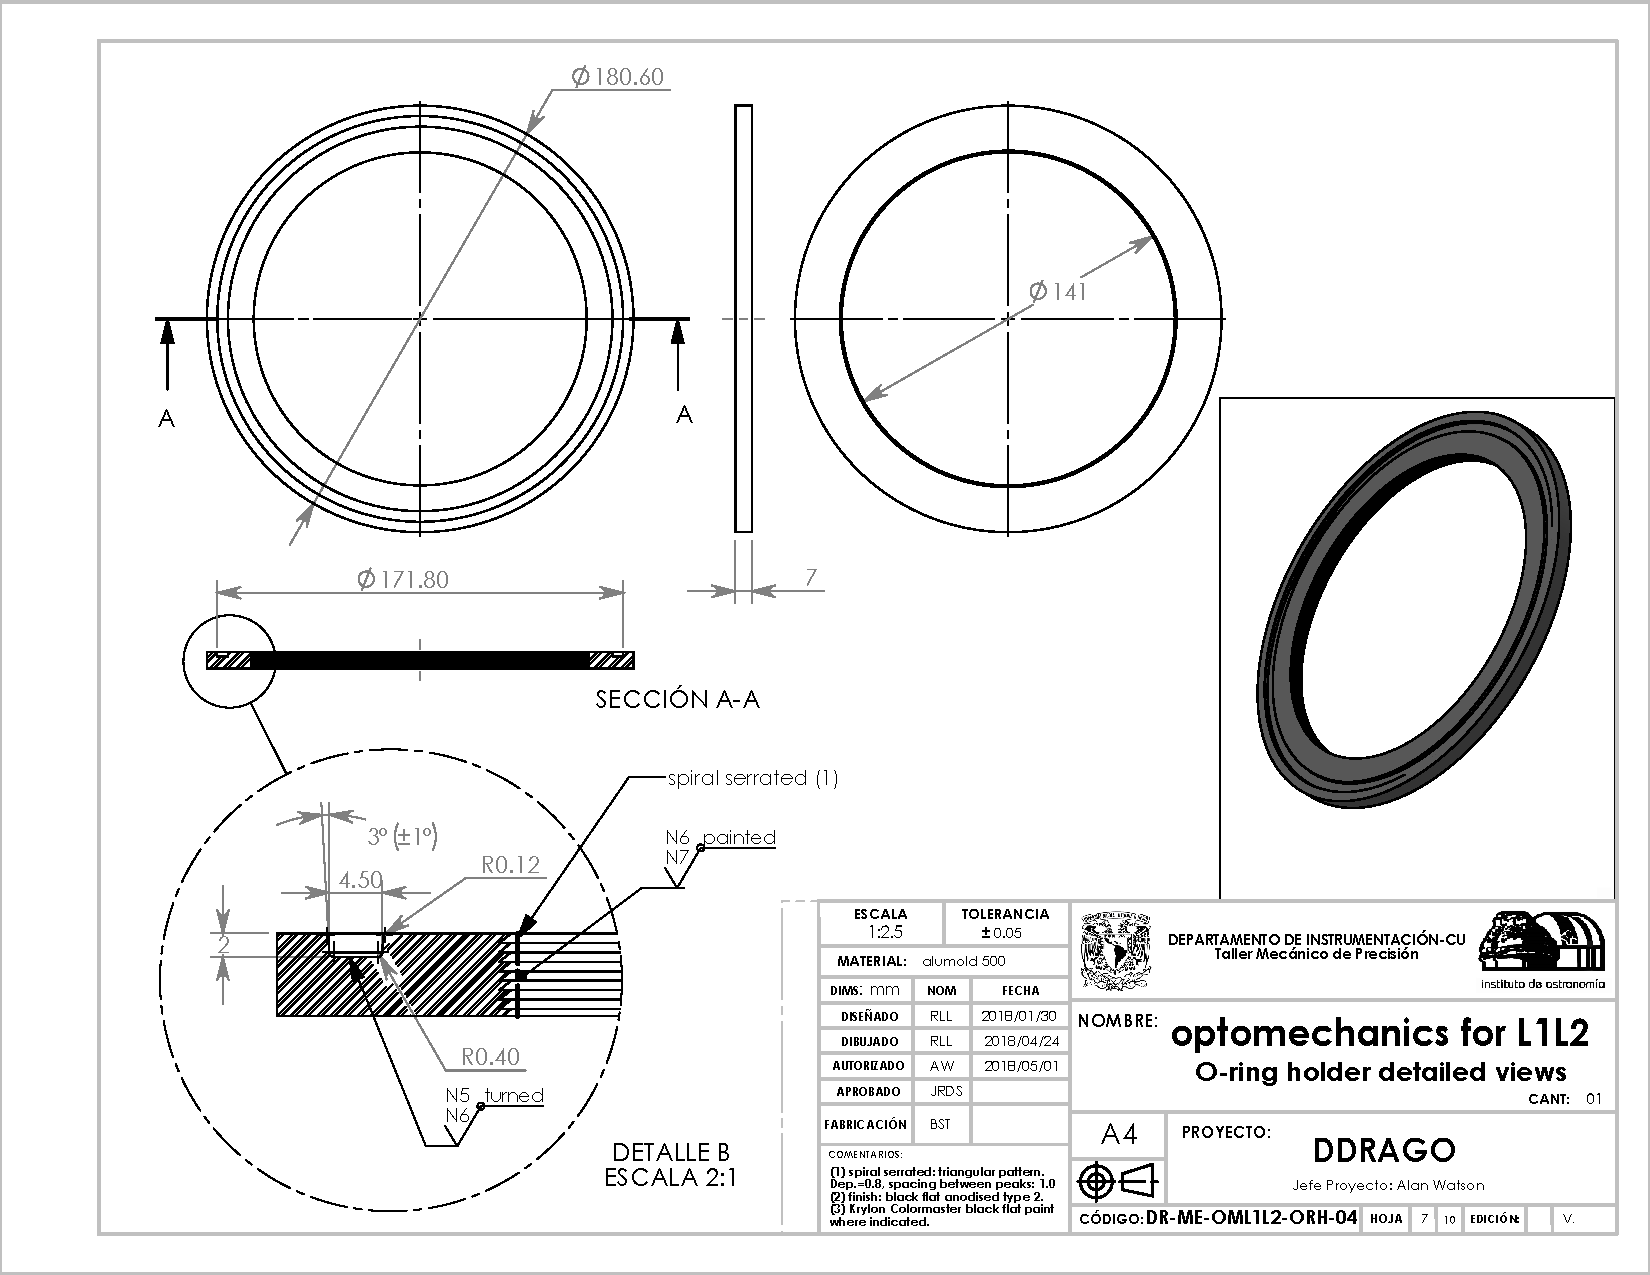
\includegraphics[height=\linewidth,angle=90]{figures/DR-ME-OML1L2-ORH-04}
\end{center}
\caption{The DR-ME-OML1L2 Barrel for L1 and L2: The DR-ME-OML1L2-ORH O-Ring Holder}
\label{figure:rosalia-oml1l2-orh}
\end{figure}

\begin{figure}
\begin{center}
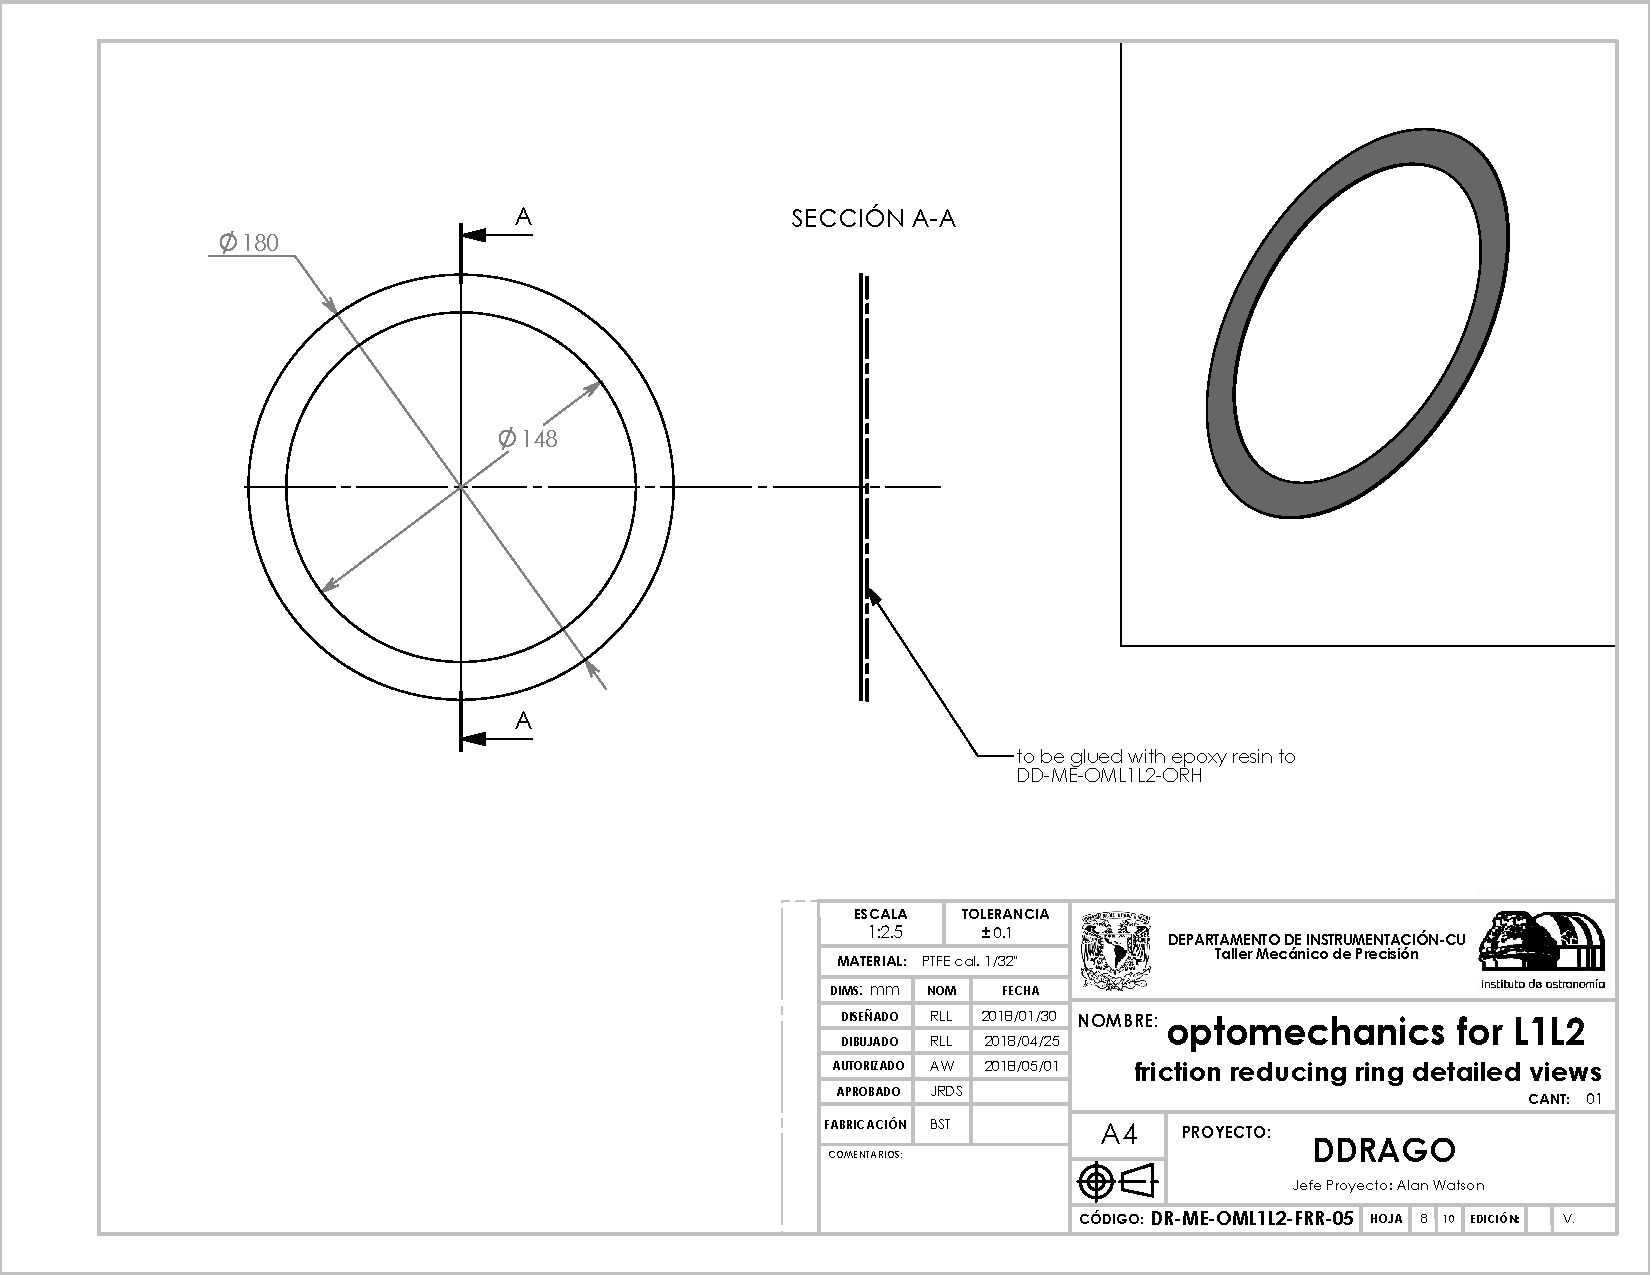
\includegraphics[height=\linewidth,angle=90]{figures/DR-ME-OML1L2-FRR-05}
\end{center}
\caption{The DR-ME-OML1L2 Barrel for L1 and L2: The DR-ME-OML1L2-FRR Friction-Reducing Ring}
\label{figure:rosalia-oml1l2-frr}
\end{figure}

\begin{figure}
\begin{center}
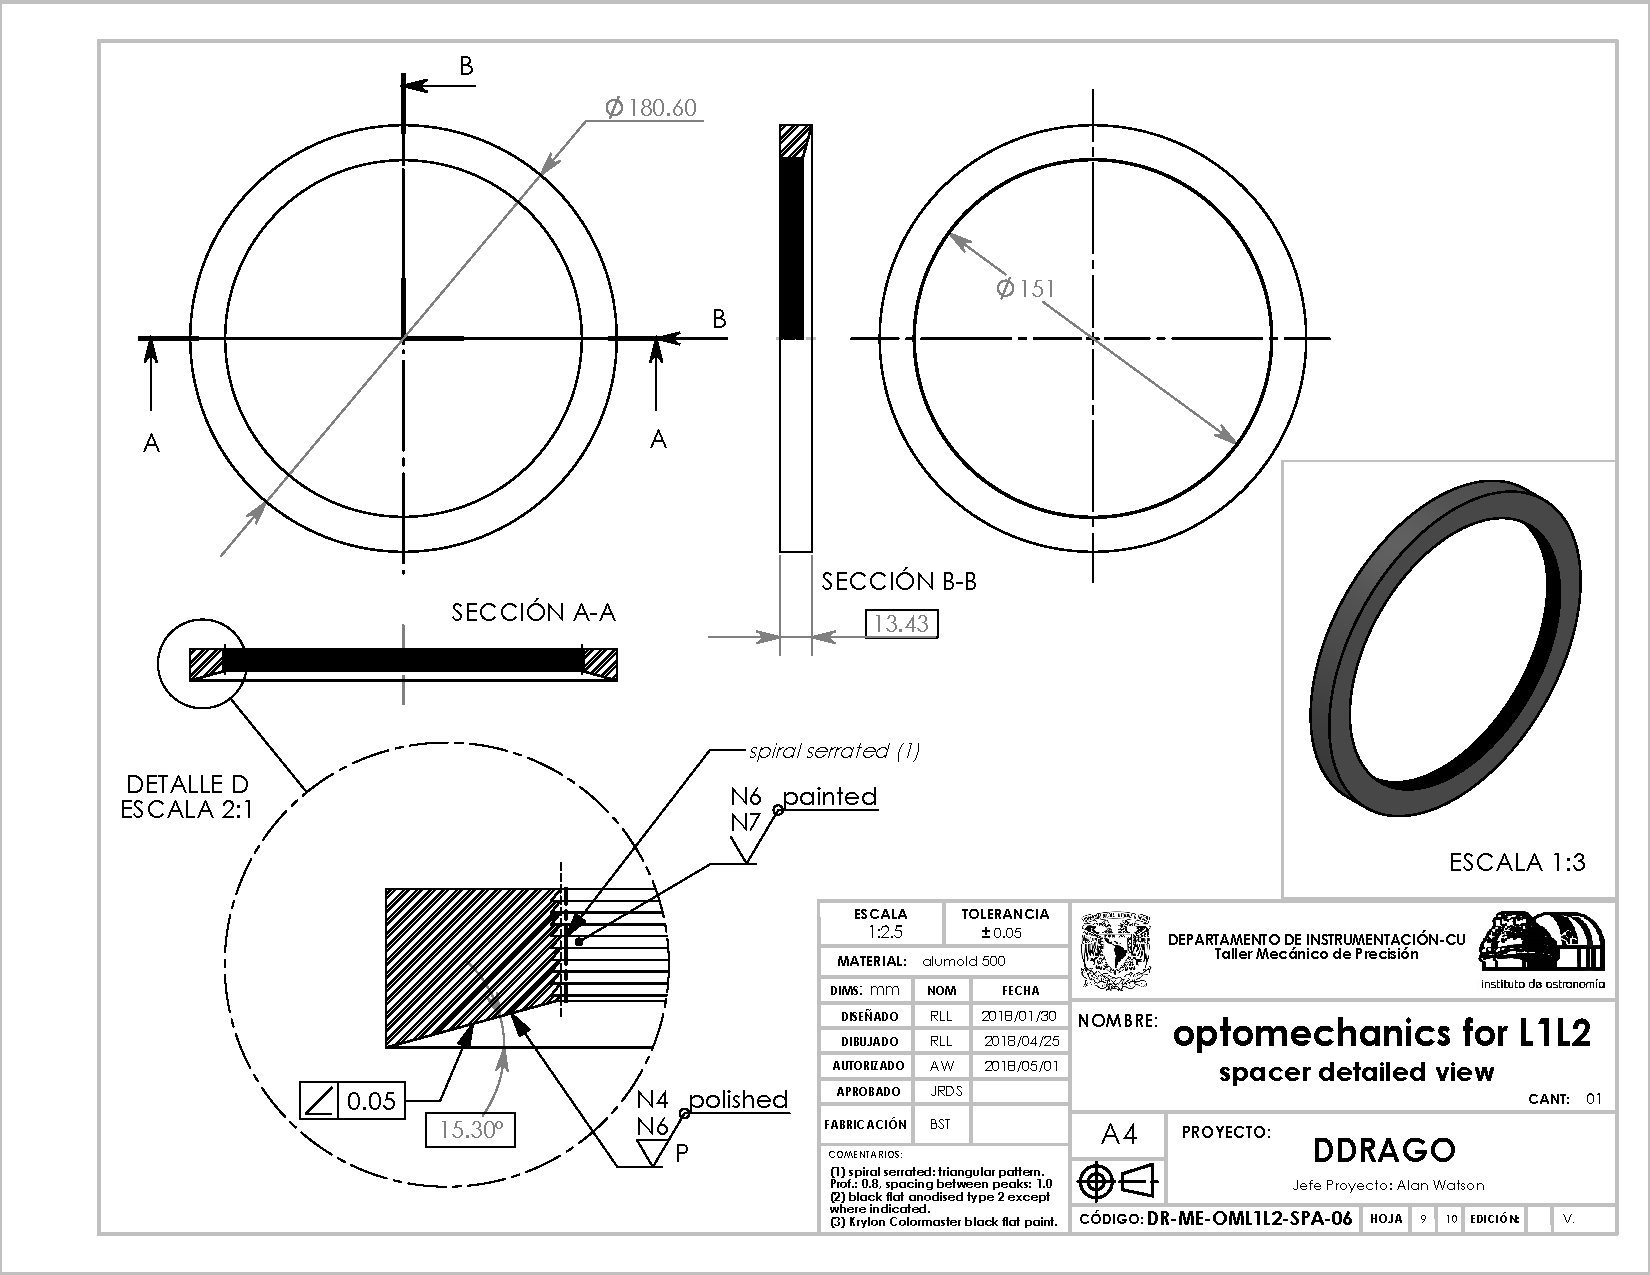
\includegraphics[height=\linewidth,angle=90]{figures/DR-ME-OML1L2-SPA-06.PDF}
\end{center}
\caption{The DR-ME-OML1L2 Barrel for L1 and L2: The DR-ME-OML1L2-SPA Spacer}
\label{figure:rosalia-oml1l2-spa}
\end{figure}

\begin{figure}
\begin{center}
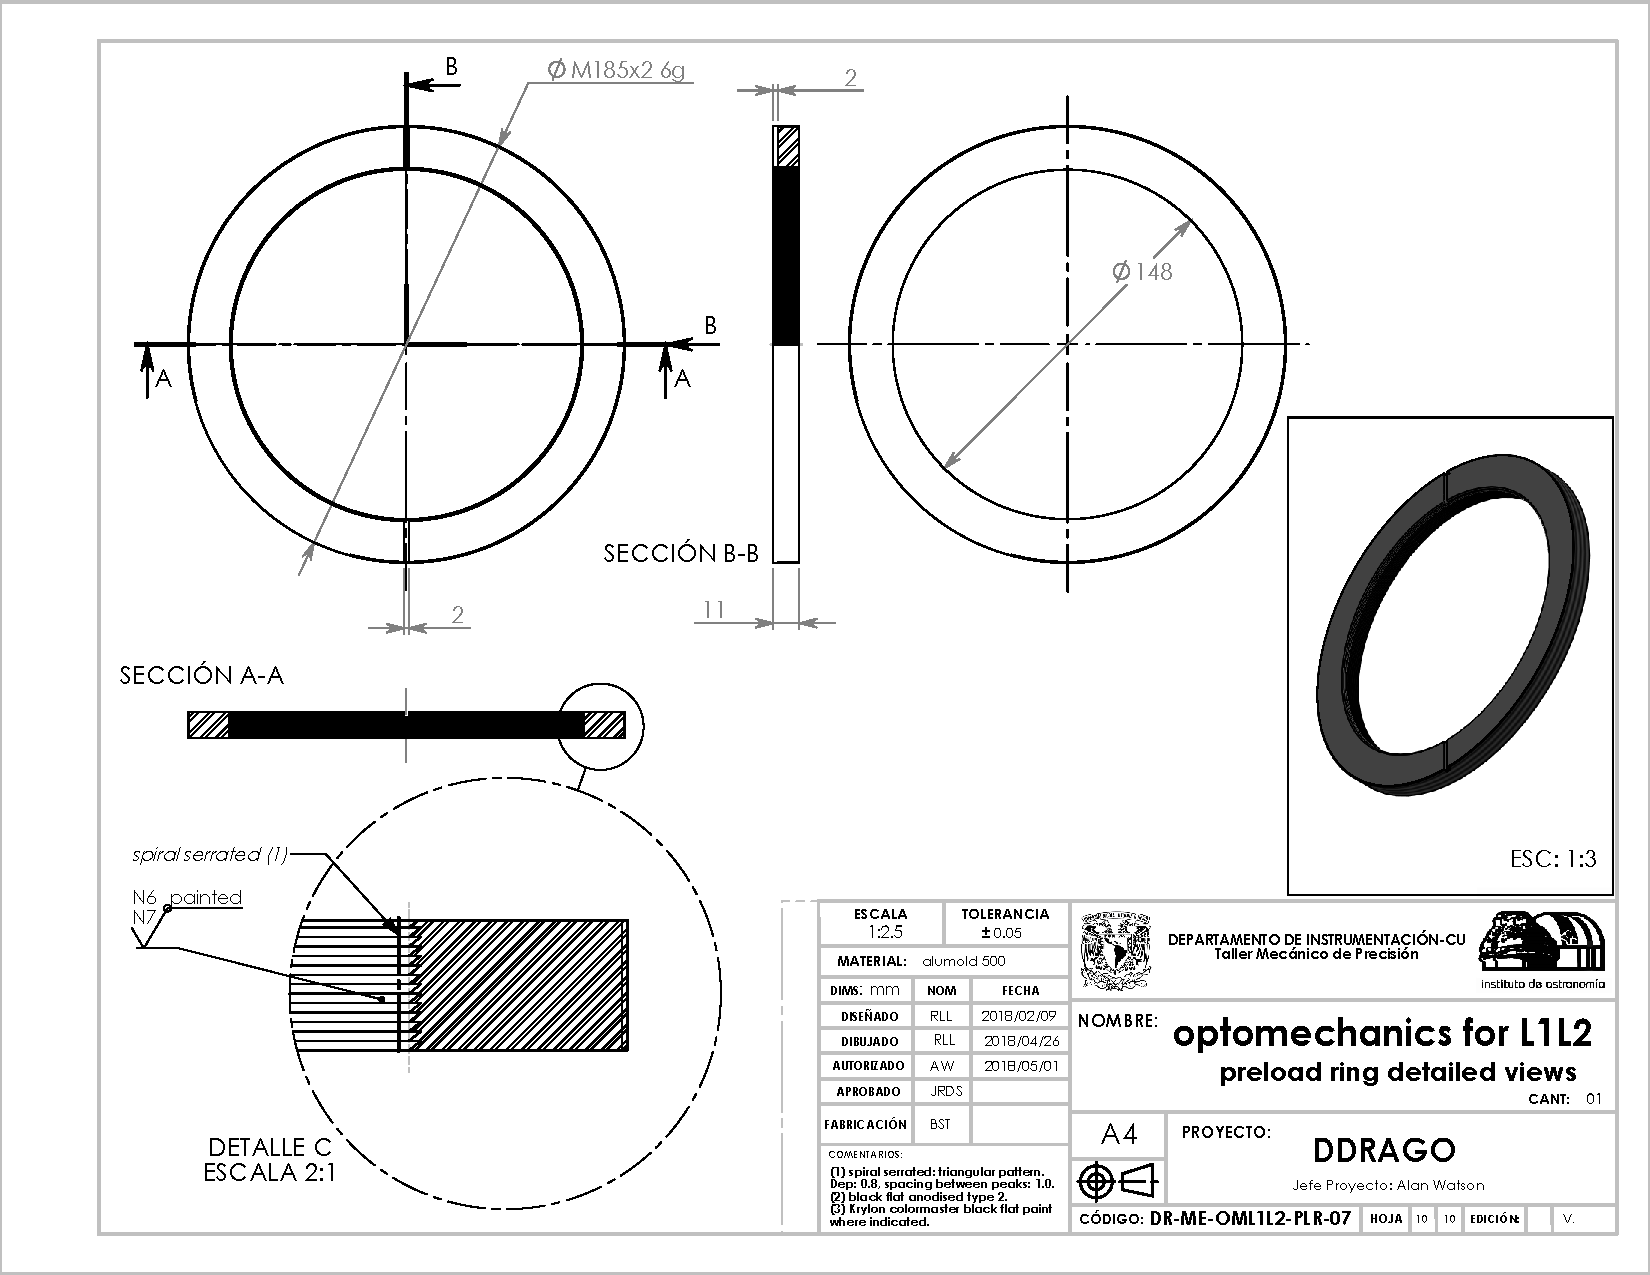
\includegraphics[height=\linewidth,angle=90]{figures/DR-ME-OML1L2-PLR-07}
\end{center}
\caption{The DR-ME-OML1L2 Barrel for L1 and L2: The DR-ME-OML1L2-PLR Preload Ring}
\label{figure:rosalia-oml1l2-plr}
\end{figure}

L1+L2 is a doublet of meniscus lenses L1 in {\CaF} and L2 in N-BaK4 both with a diameter of 180 mm. The group constitutes the common doublet for DDRAGO and CAGIRE. The design of the lens barrel is shown in Figures~\ref{figure:rosalia-oml1l2-perspective} to \ref{figure:rosalia-oml1l2-thermal-ring} and plans of the individual parts are shown in Figures~\ref{figure:rosalia-oml1l2-bar} to \ref{figure:rosalia-oml1l2-plr}.

The barrel has a flange that will allow it to be directly attached to the support structure (see Figure \ref{figure:alex-ss-fp1}). When the instrument is mounted on the telescope, the barrel will extend into the derotator. 

On its front surface, the barrel has a set of threaded holes to receive the mount for the spherical testing mirror STM (see Figure~\ref{figure:alex-omstm}).

The first surface of L1 is convex and makes contact with a conical shoulder that is machined in the barrel and provides tangential support. Between L1 and L2 there is an aluminium spacer. The first surface of this spacer makes contact with the flat bevel of L1 and the second surface of the spacer makes tangential contact with the first surface of L2. Between L2 and the retaining ring there is the thermal ring, a silicone O-ring having a section diameter of 3.5 mm (Parker® number 2-260 S0604-70). The torque applied during assembly on the preload ring will give the required preload and will compress the O-ring by about 30\% at maximum compression. 

The barrel has threaded holes for twelve centering set-screws, giving $x$ and $y$ adjustments of L1, the spacer, and L2. These holes are in the planes of the centre of gravity of each lens and the spacer in order to have a precise control of their positions.

\subsubsection{The DR-ME-OMSTM Mount for STM}

\begin{figure}
\begin{center}
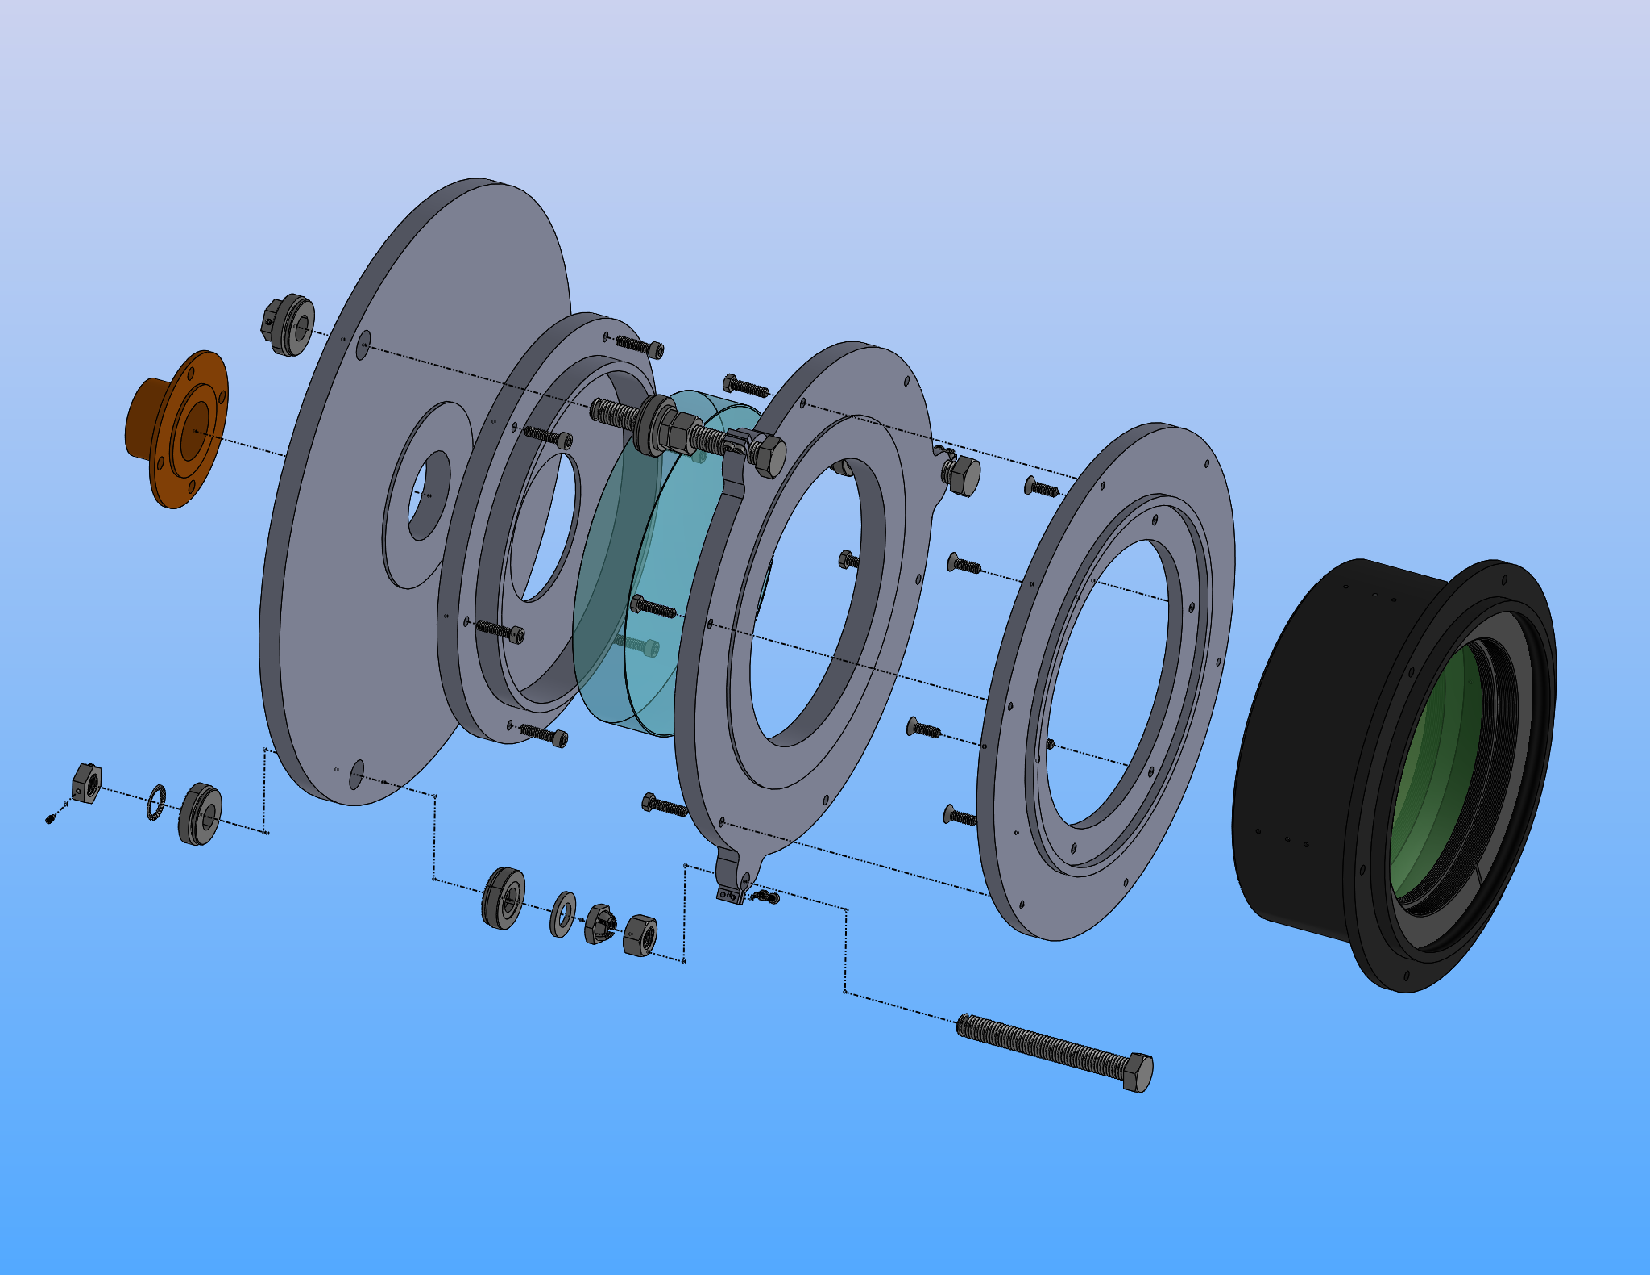
\includegraphics[width=\linewidth]{figures/DR-ME-OMSTM-OML1L2-REN.PDF}
\end{center}
\caption{The DR-ME-OML1L2 Barrel (right) with the DR-ME-OMSTM mounted (left).}
\label{figure:alex-omstm}
\end{figure}

The OMSTM mount is shown in Figure~\ref{figure:alex-omstm}. It attaches to the front surface of OML1L2 and supports the STM test mirror. It has a three-point adjustment mechanism to allow piston and tilt to be adjusted.

\subsubsection{The DR-ME-OML3 Mount for L3}

\begin{figure}
\begin{center}
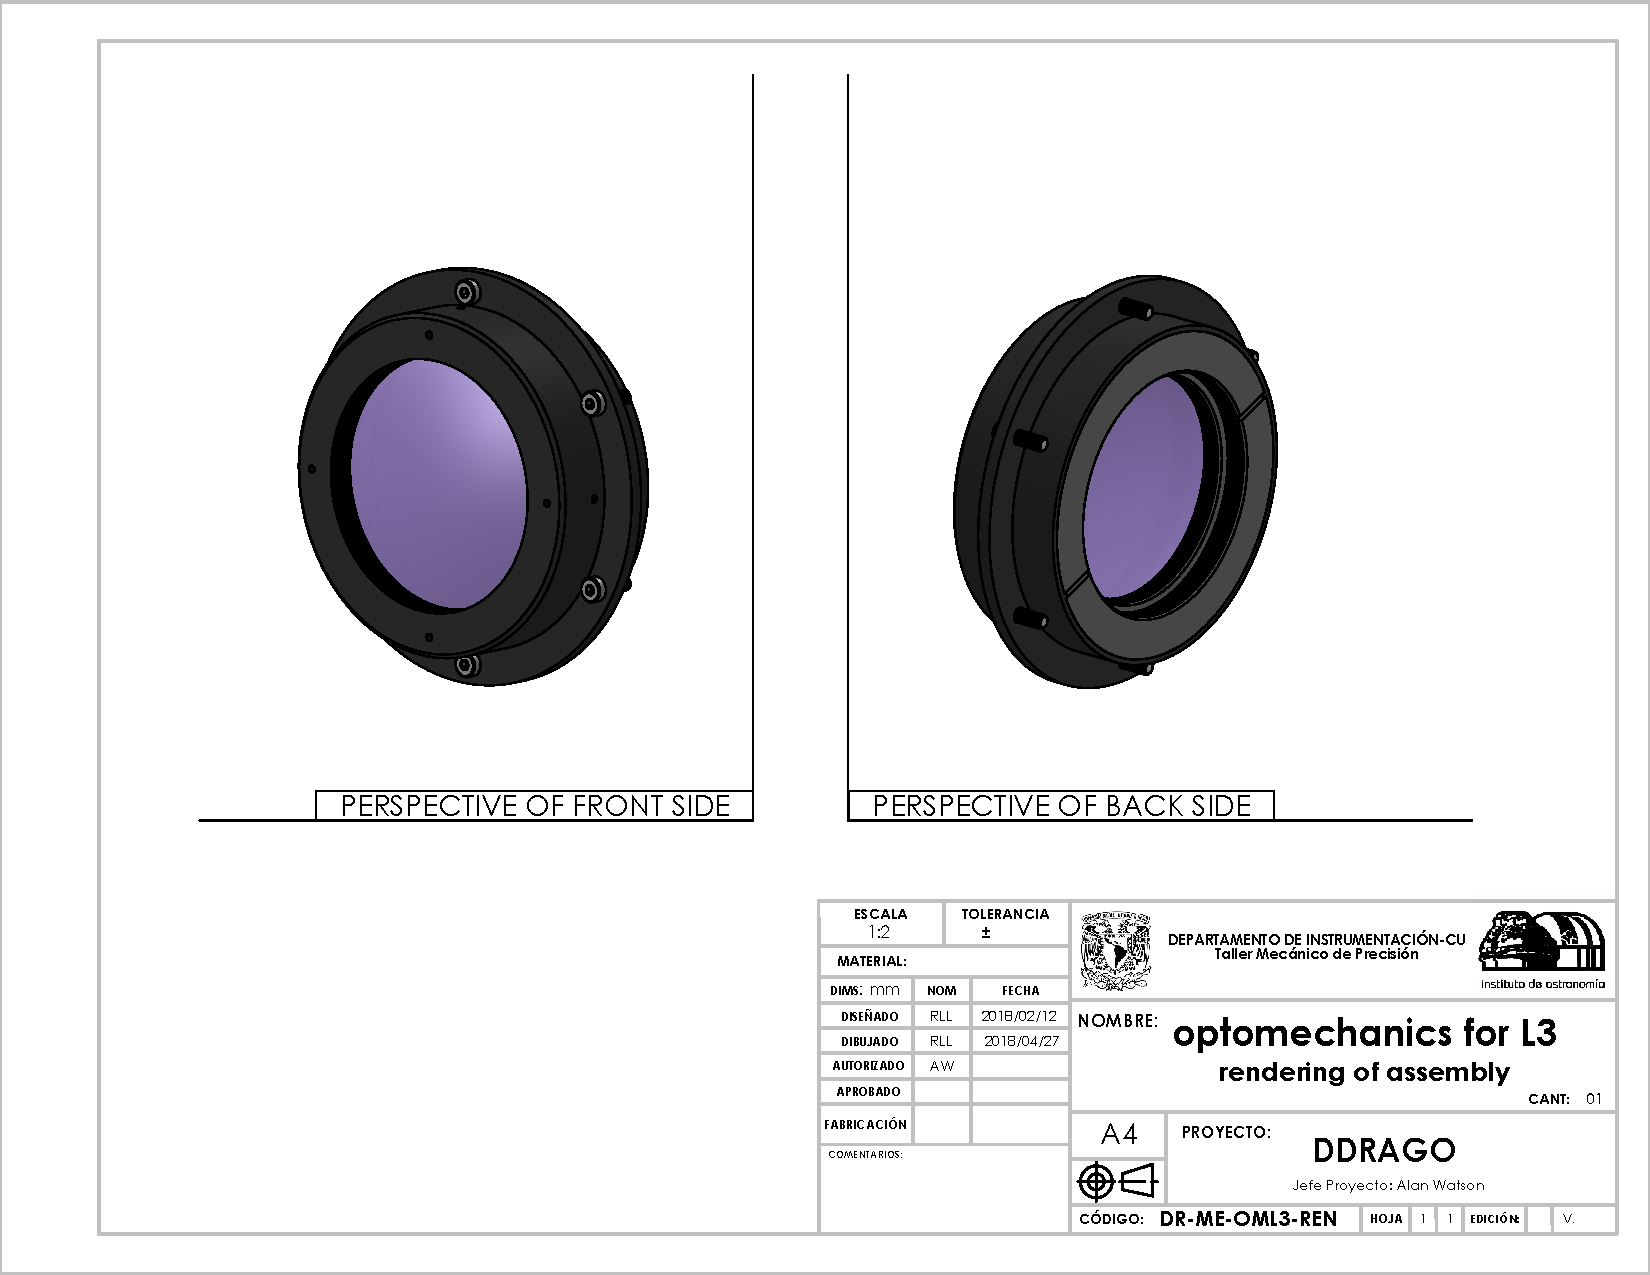
\includegraphics[height=\linewidth,angle=90]{figures/DR-ME-OML3-REN}
\end{center}
\caption{The DR-ME-OML3 Barrel for L3: Perspective}
\label{figure:rosalia-oml3-perspective}
\end{figure}

\begin{figure}
\begin{center}
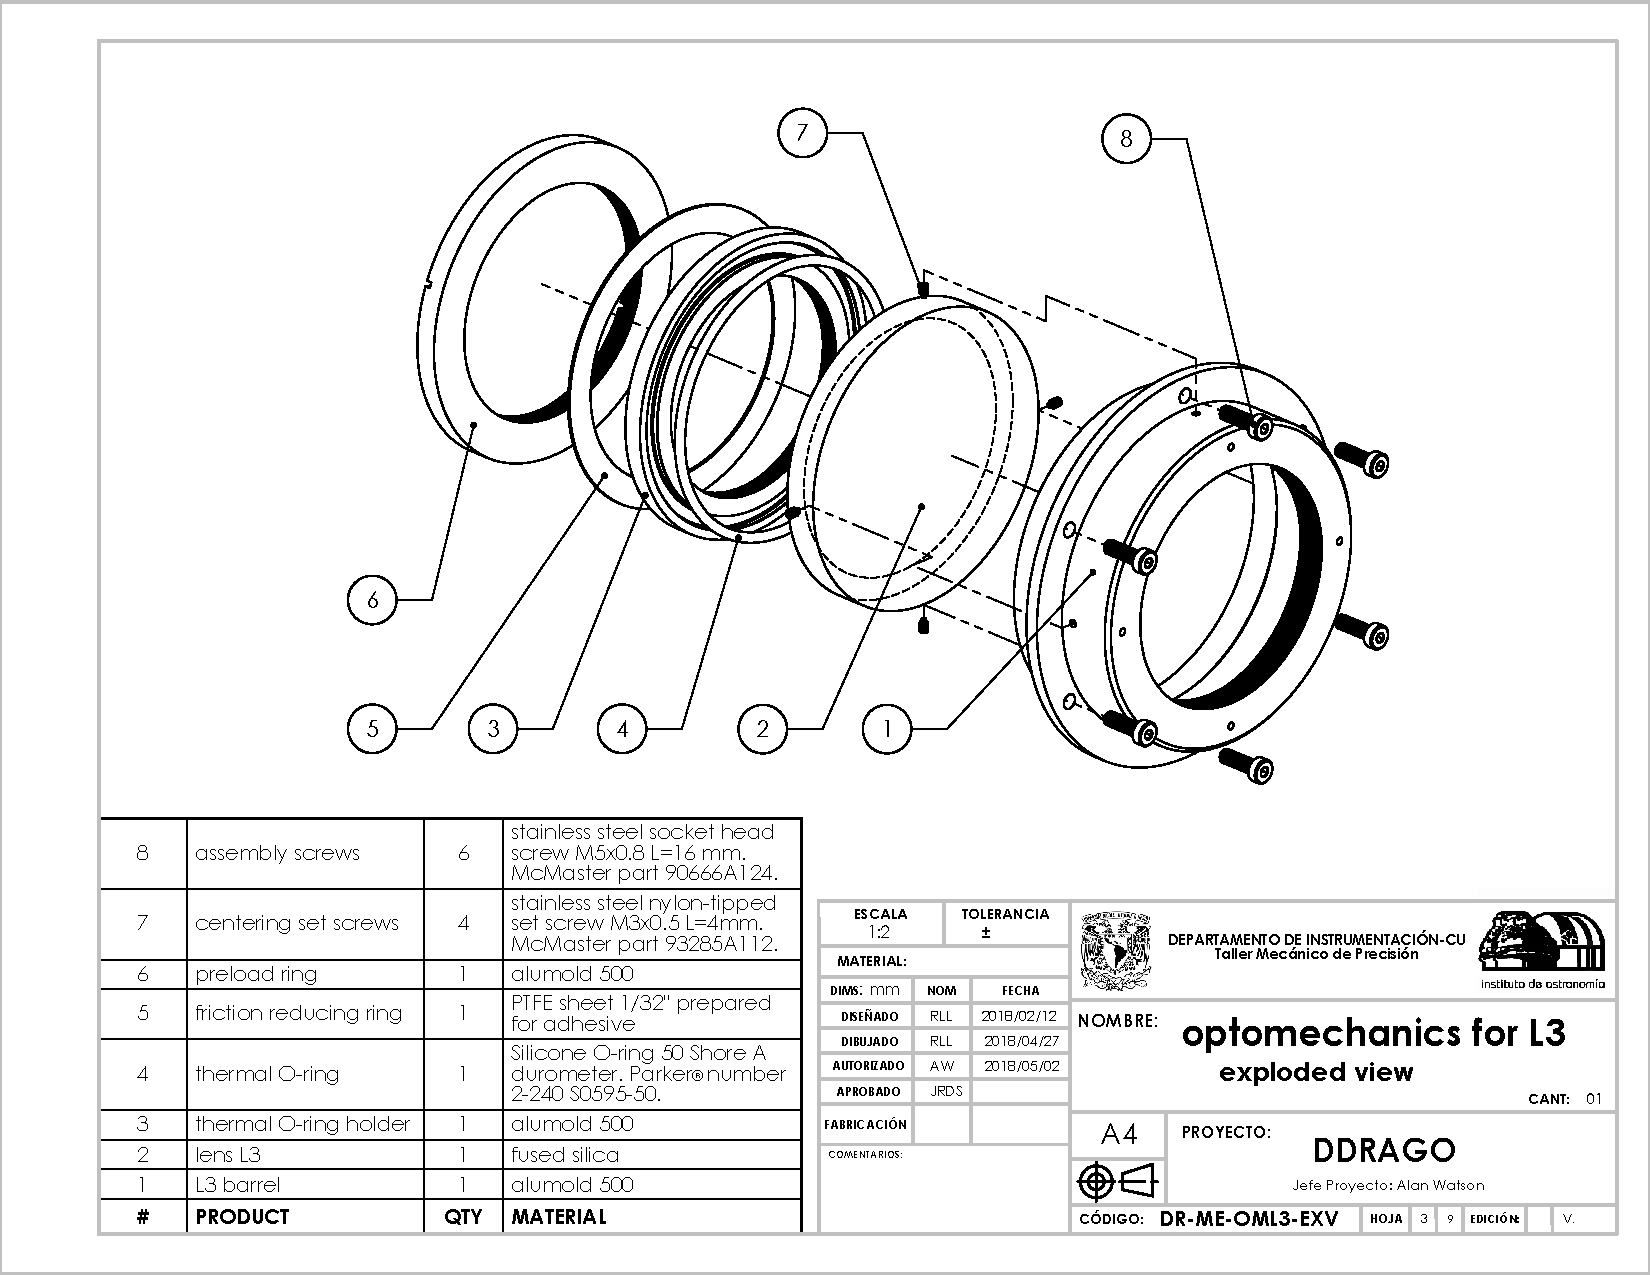
\includegraphics[height=\linewidth,angle=90]{figures/DR-ME-OML3-EXV}
\end{center}
\caption{The DR-ME-OML3 Barrel for L3: Exploded View}
\label{figure:rosalia-oml3-exploded}
\end{figure}

\begin{figure}
\begin{center}
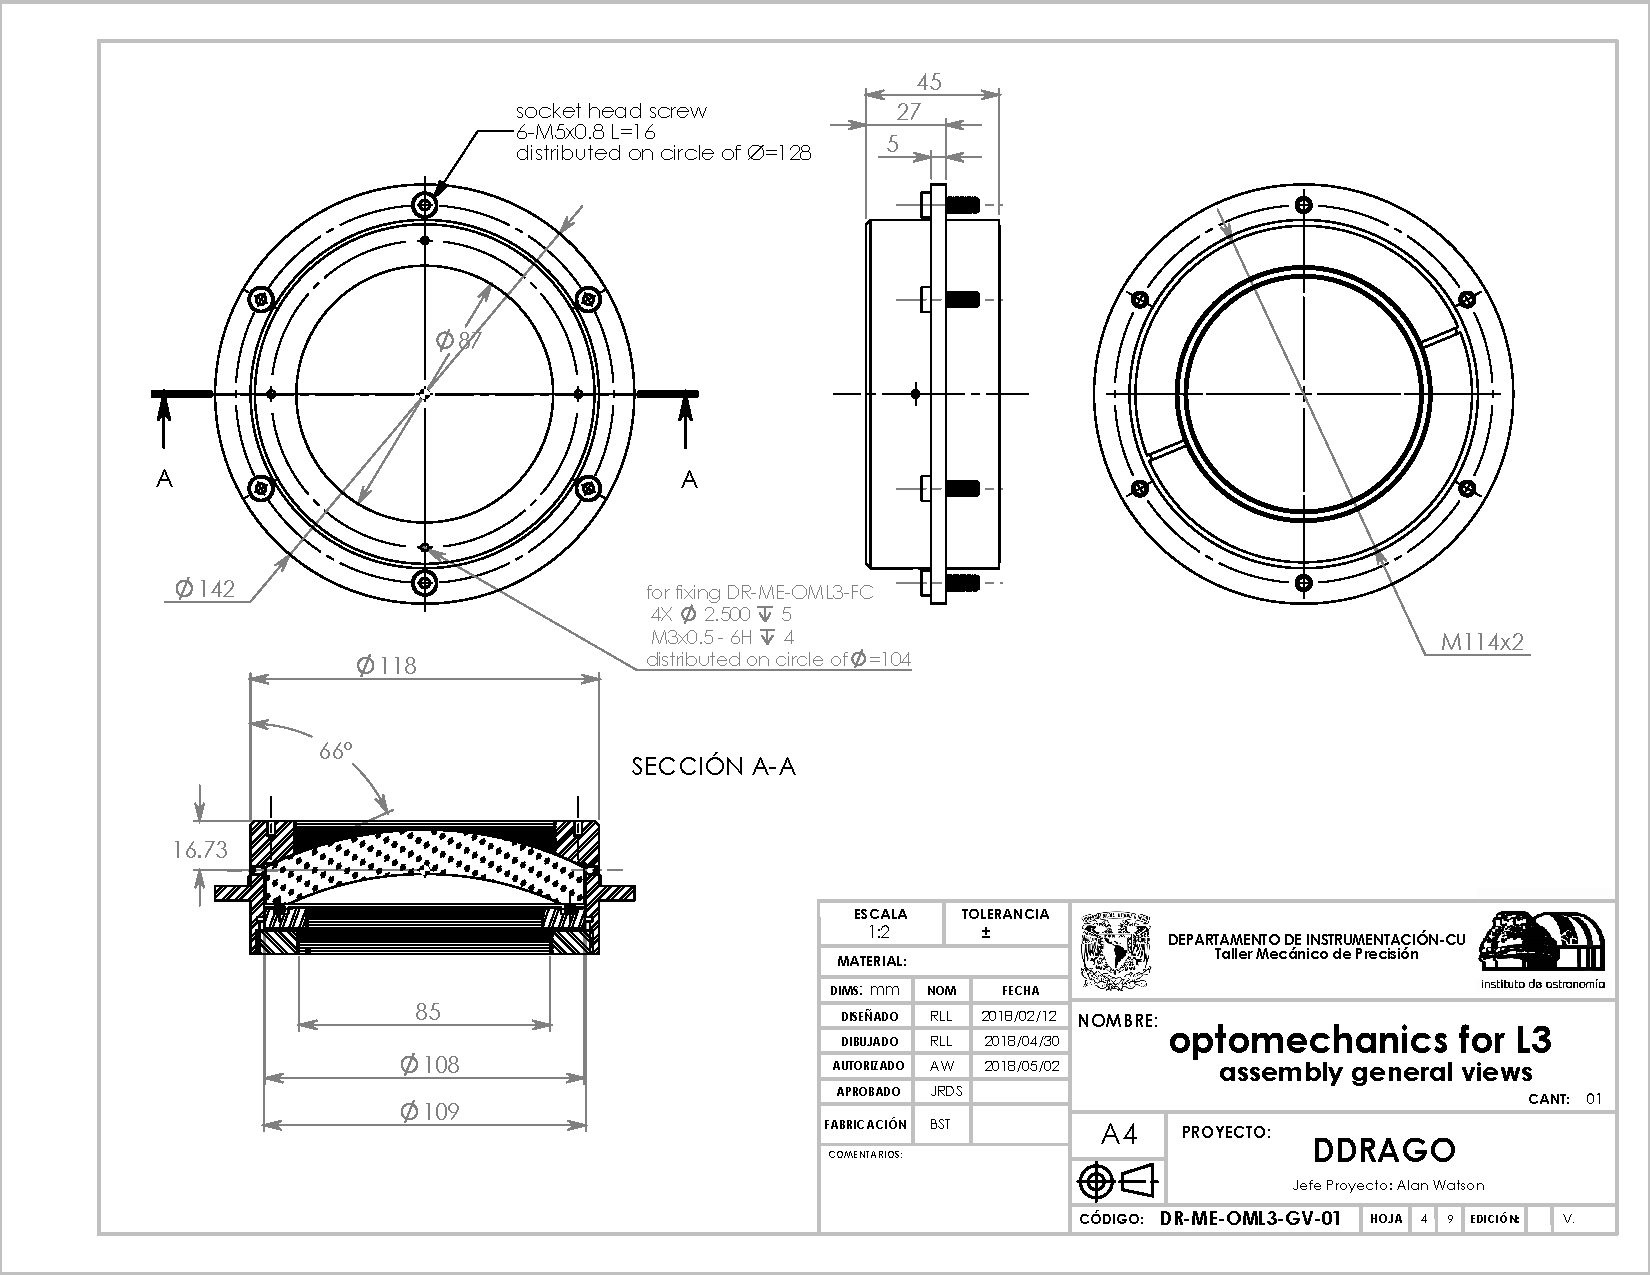
\includegraphics[height=\linewidth,angle=90]{figures/DR-ME-OML3-GV-01}
\end{center}
\caption{The DR-ME-OML3 Barrel for L3: General View}
\label{figure:rosalia-oml3-general}
\end{figure}

\begin{figure}
\begin{center}
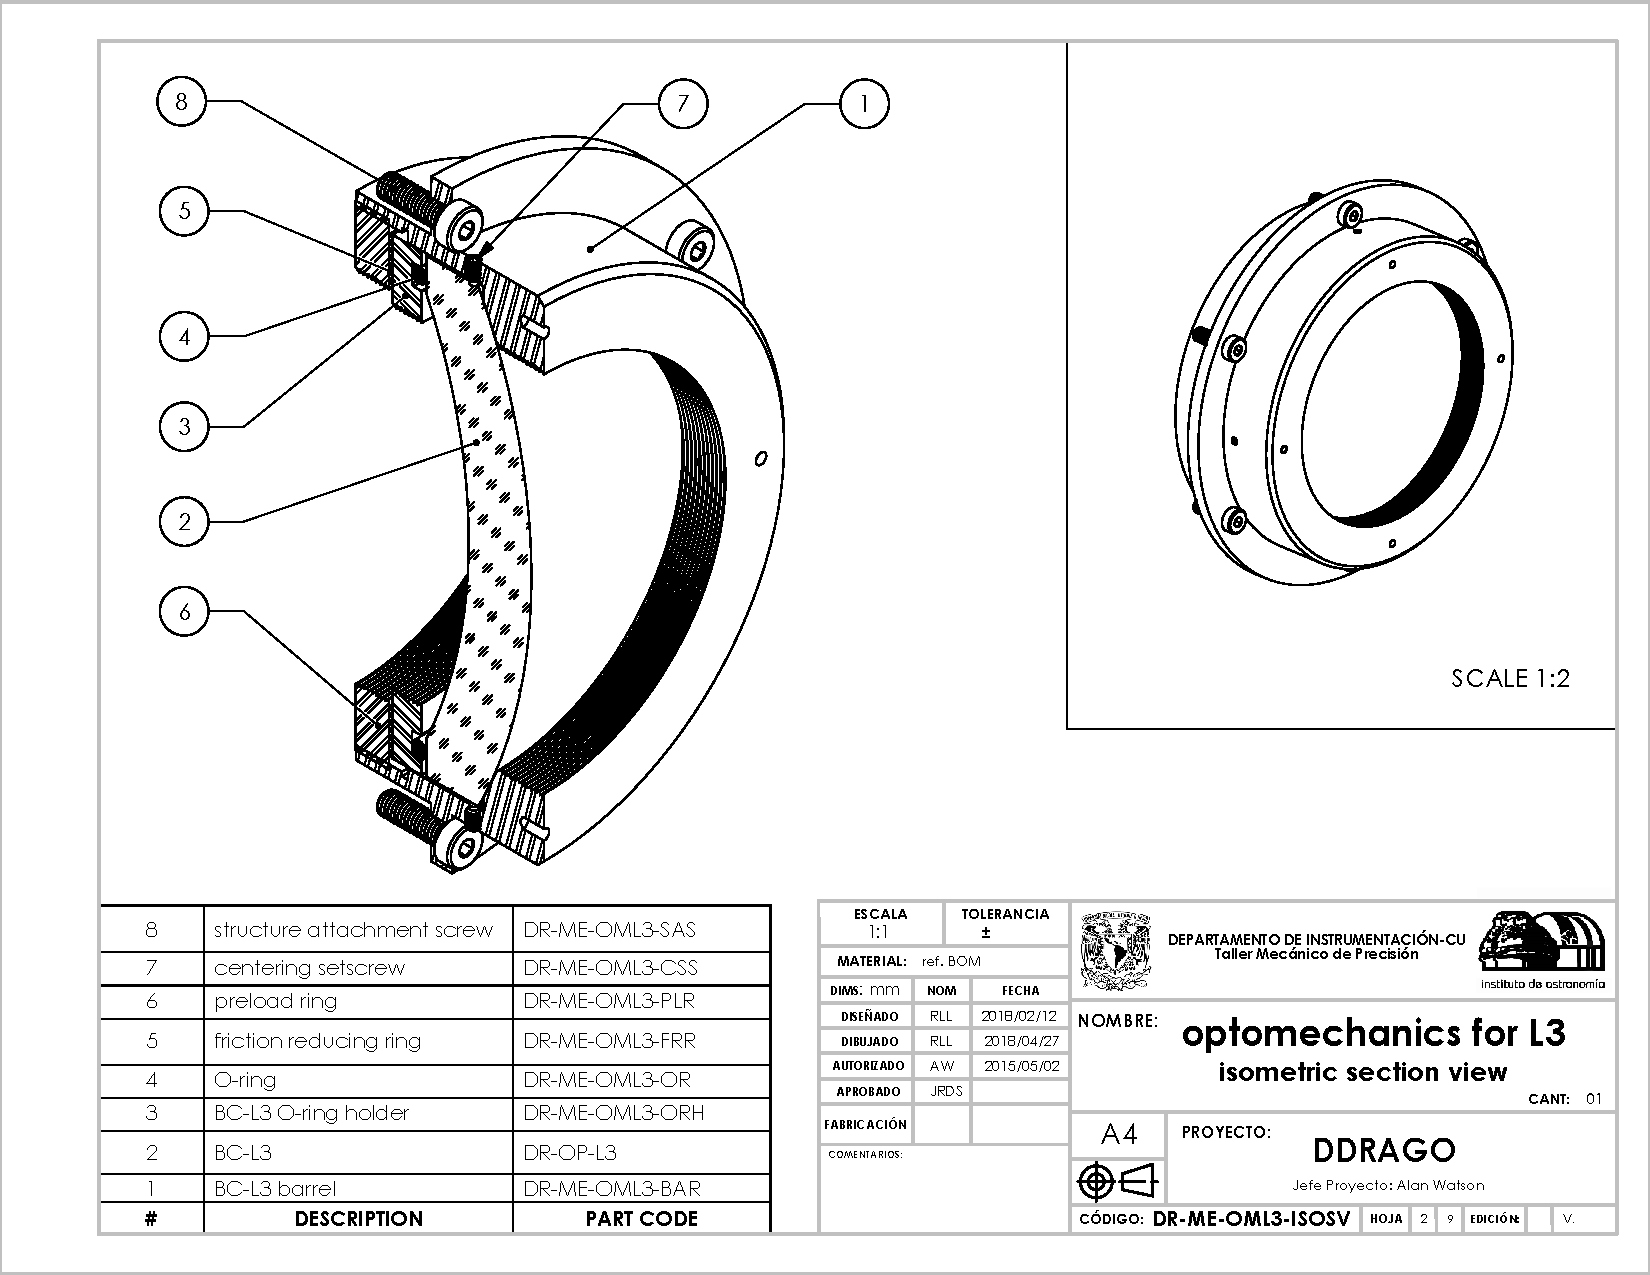
\includegraphics[height=\linewidth,angle=90]{figures/DR-ME-OML3-ISOSV}
\end{center}
\caption{The DR-ME-OML3 Barrel for L3: Section View}
\label{figure:rosalia-oml3-section}
\end{figure}

\begin{figure}
\begin{center}
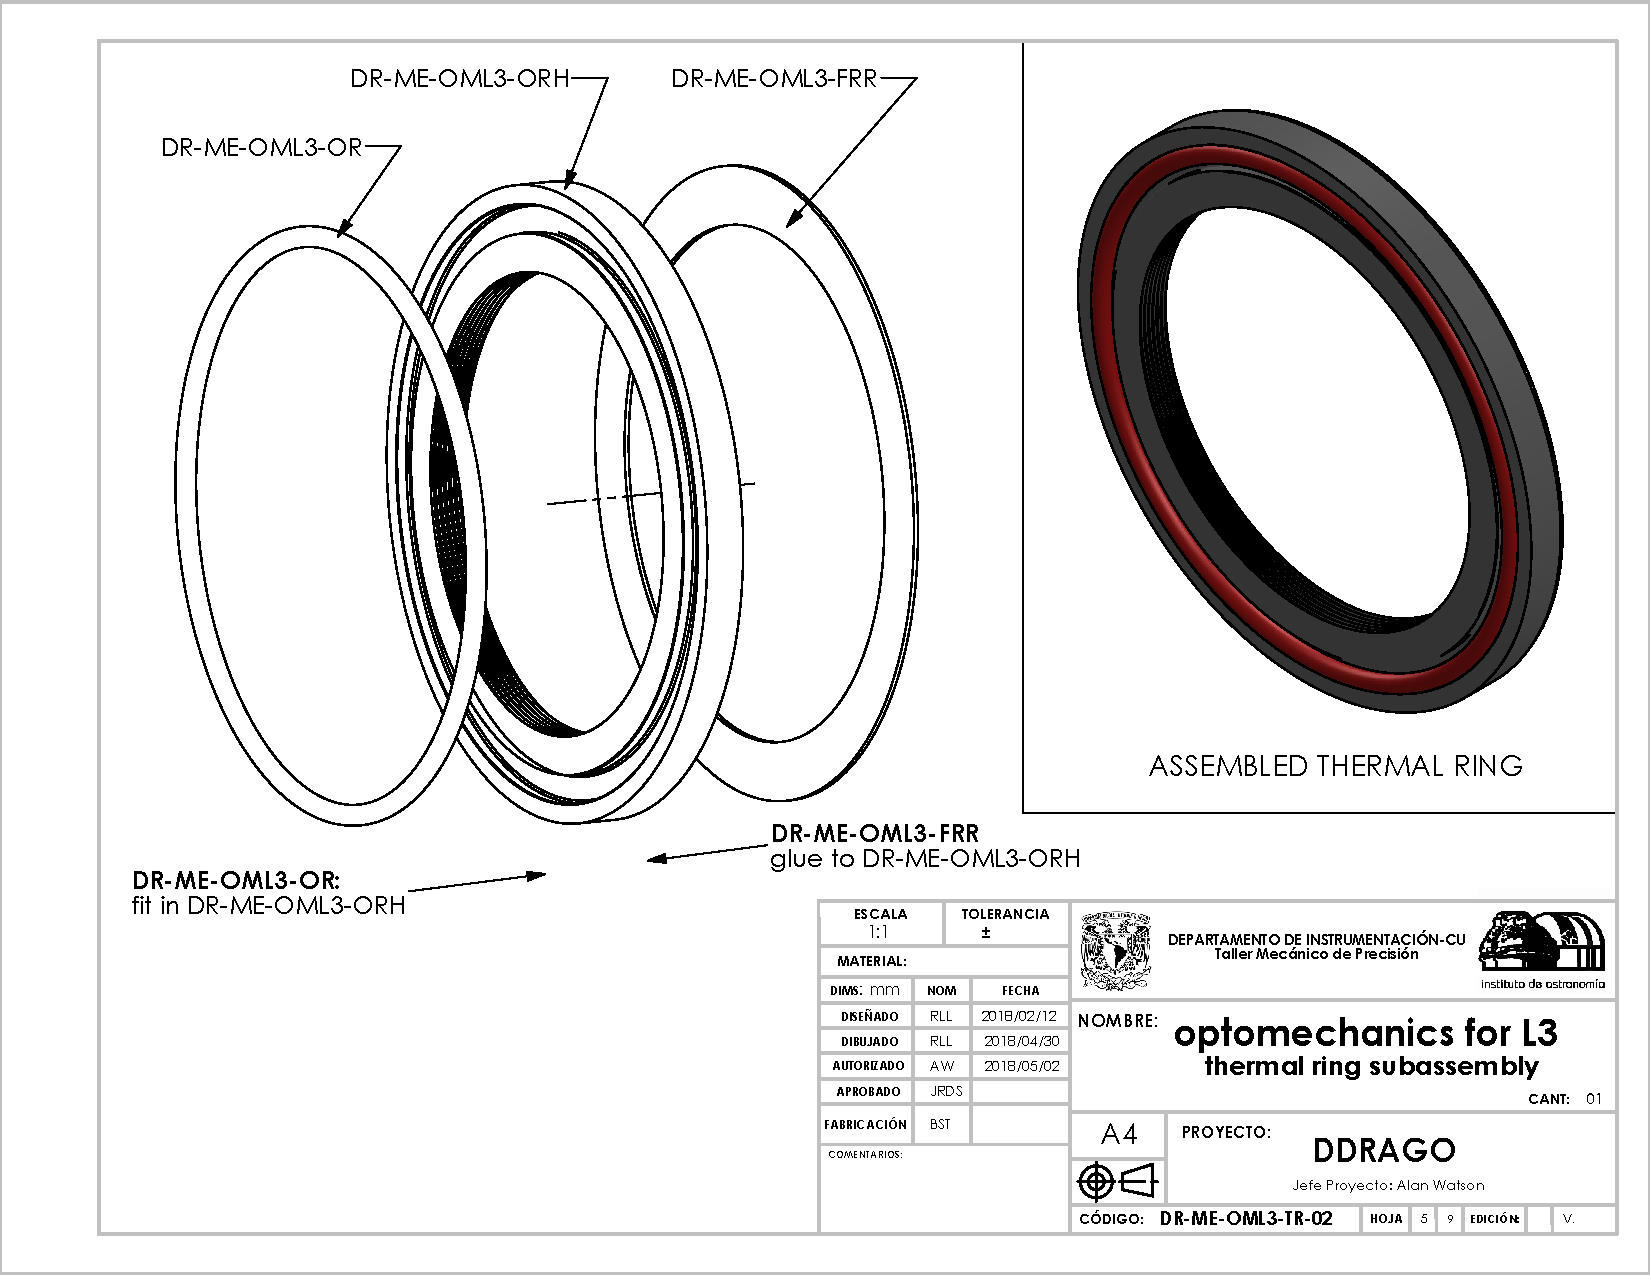
\includegraphics[height=\linewidth,angle=90]{figures/DR-ME-OML3-TR-02}
\end{center}
\caption{The DR-ME-OML3 Barrel for L3: The DR-ME-OML3-TR Thermal Ring Assembly}
\label{figure:rosalia-oml3-thermal-ring}
\end{figure}

\begin{figure}
\begin{center}
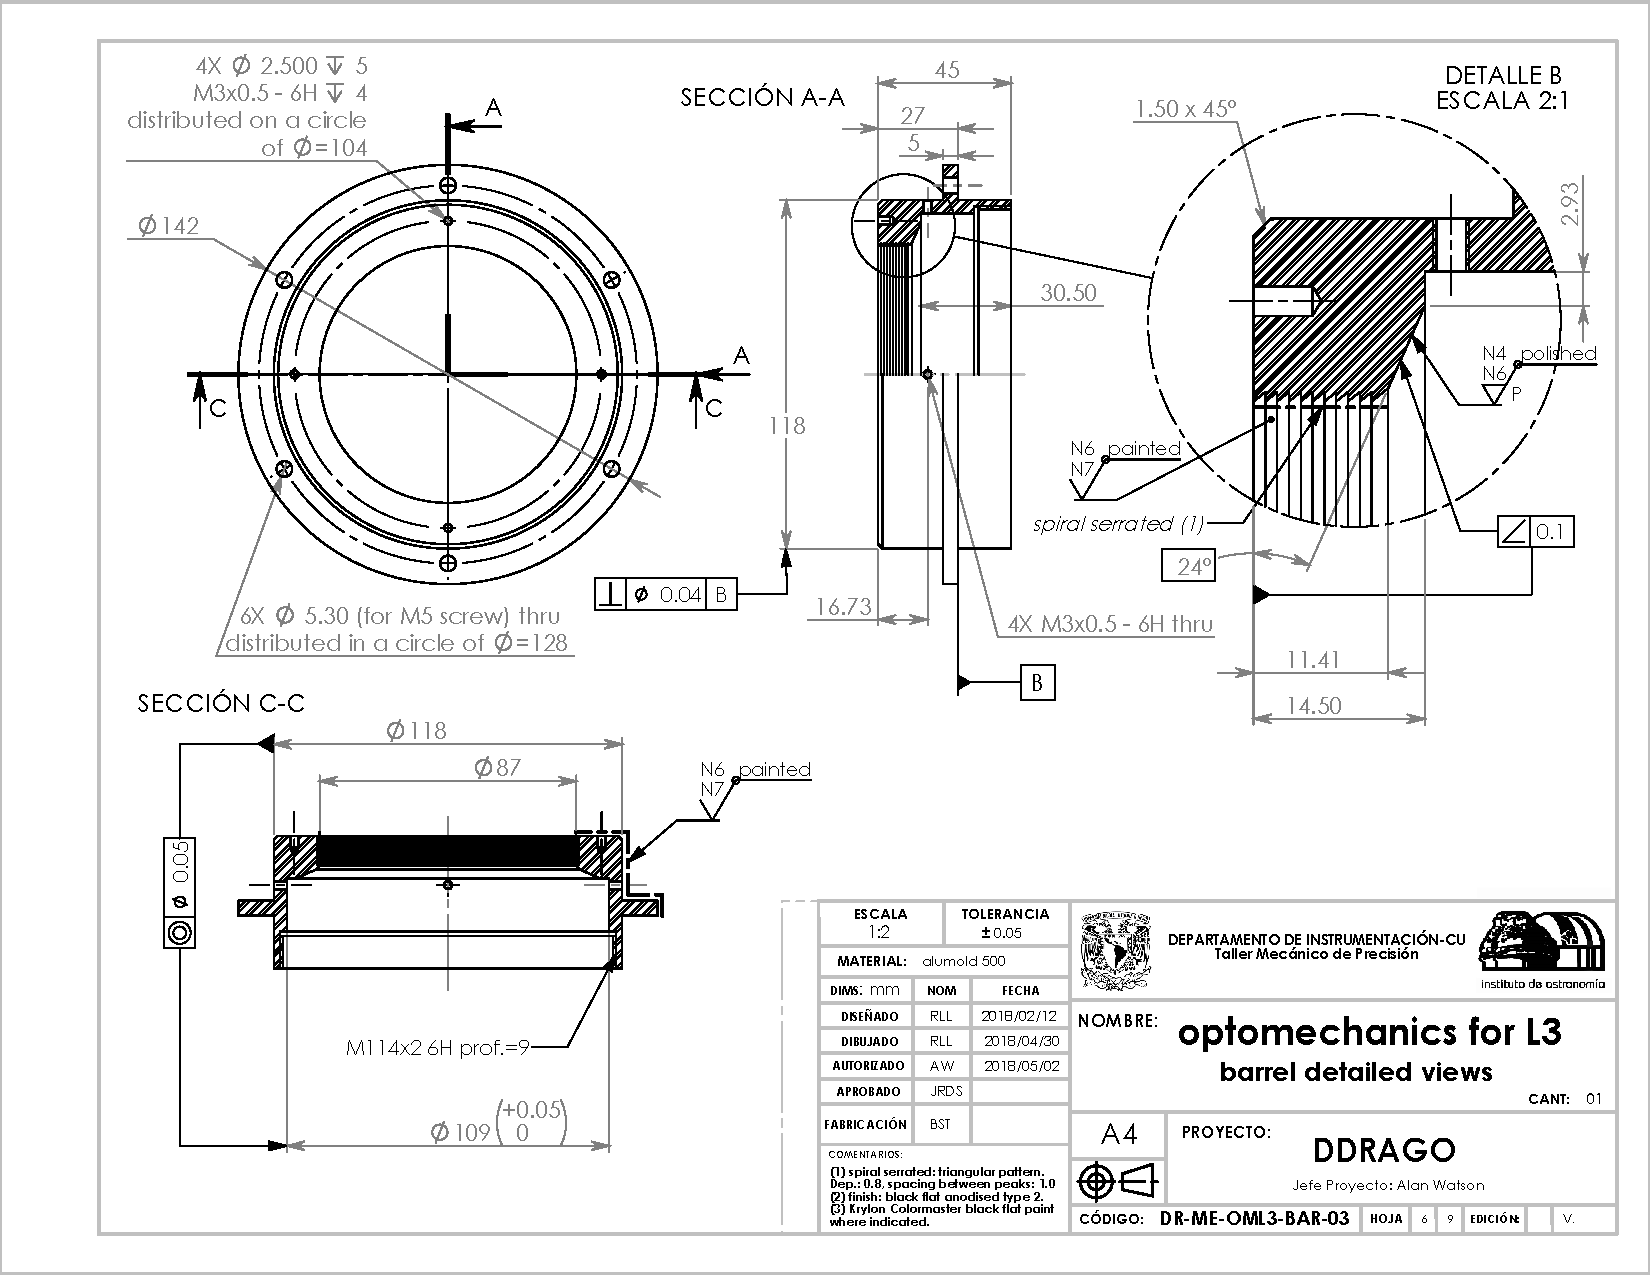
\includegraphics[height=\linewidth,angle=90]{figures/DR-ME-OML3-BAR-03}
\end{center}
\caption{The DR-ME-OML3 Barrel for L3: The DR-ME-OML3-BAR Barrel}
\label{figure:rosalia-oml3-bar}
\end{figure}

\begin{figure}
\begin{center}
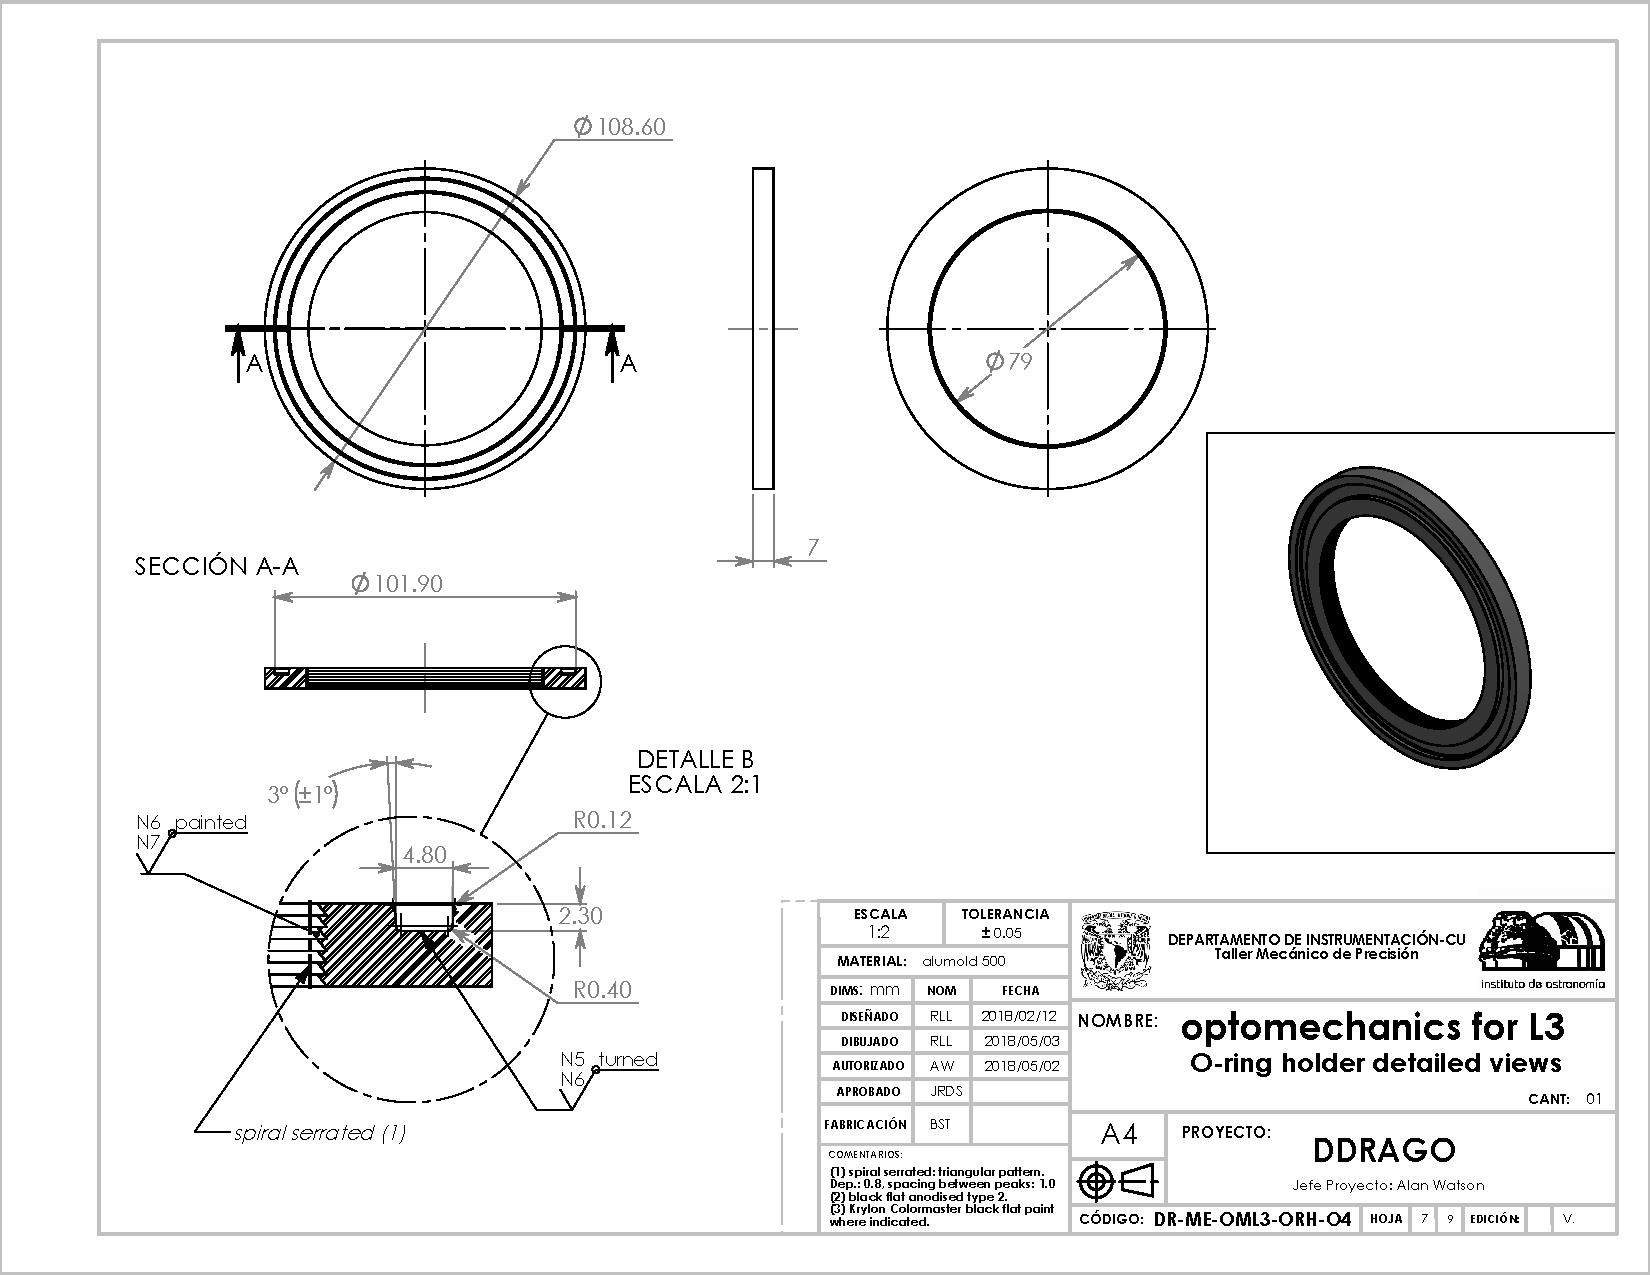
\includegraphics[height=\linewidth,angle=90]{figures/DR-ME-OML3-ORH-04}
\end{center}
\caption{The DR-ME-OML3 Barrel for L3: The DR-ME-OML3-ORH O-Ring Holder}
\label{figure:rosalia-oml3-orh}
\end{figure}

\begin{figure}
\begin{center}
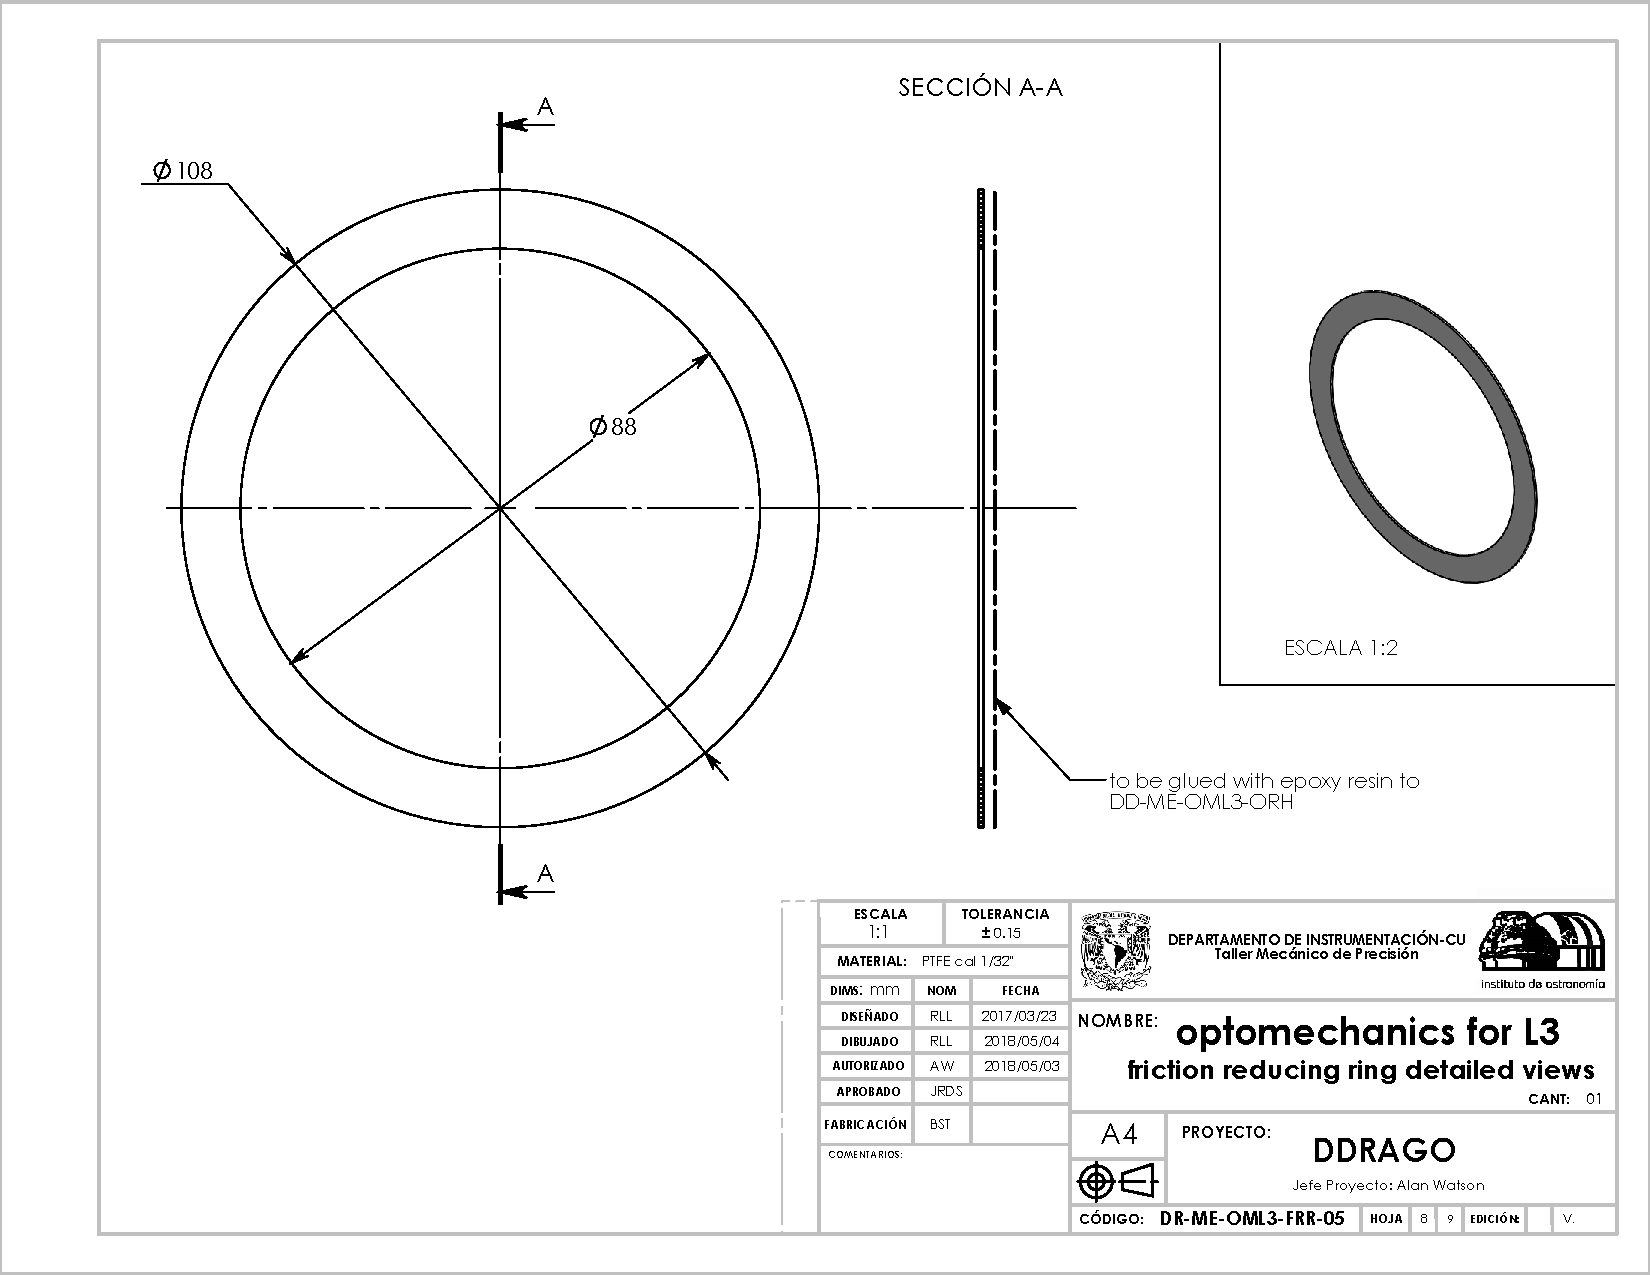
\includegraphics[height=\linewidth,angle=90]{figures/DR-ME-OML3-FRR-05}
\end{center}
\caption{The DR-ME-OML3 Barrel for L3: The DR-ME-OML3-FRR Friction-Reducing Ring}
\label{figure:rosalia-oml3-frr}
\end{figure}

\begin{figure}
\begin{center}
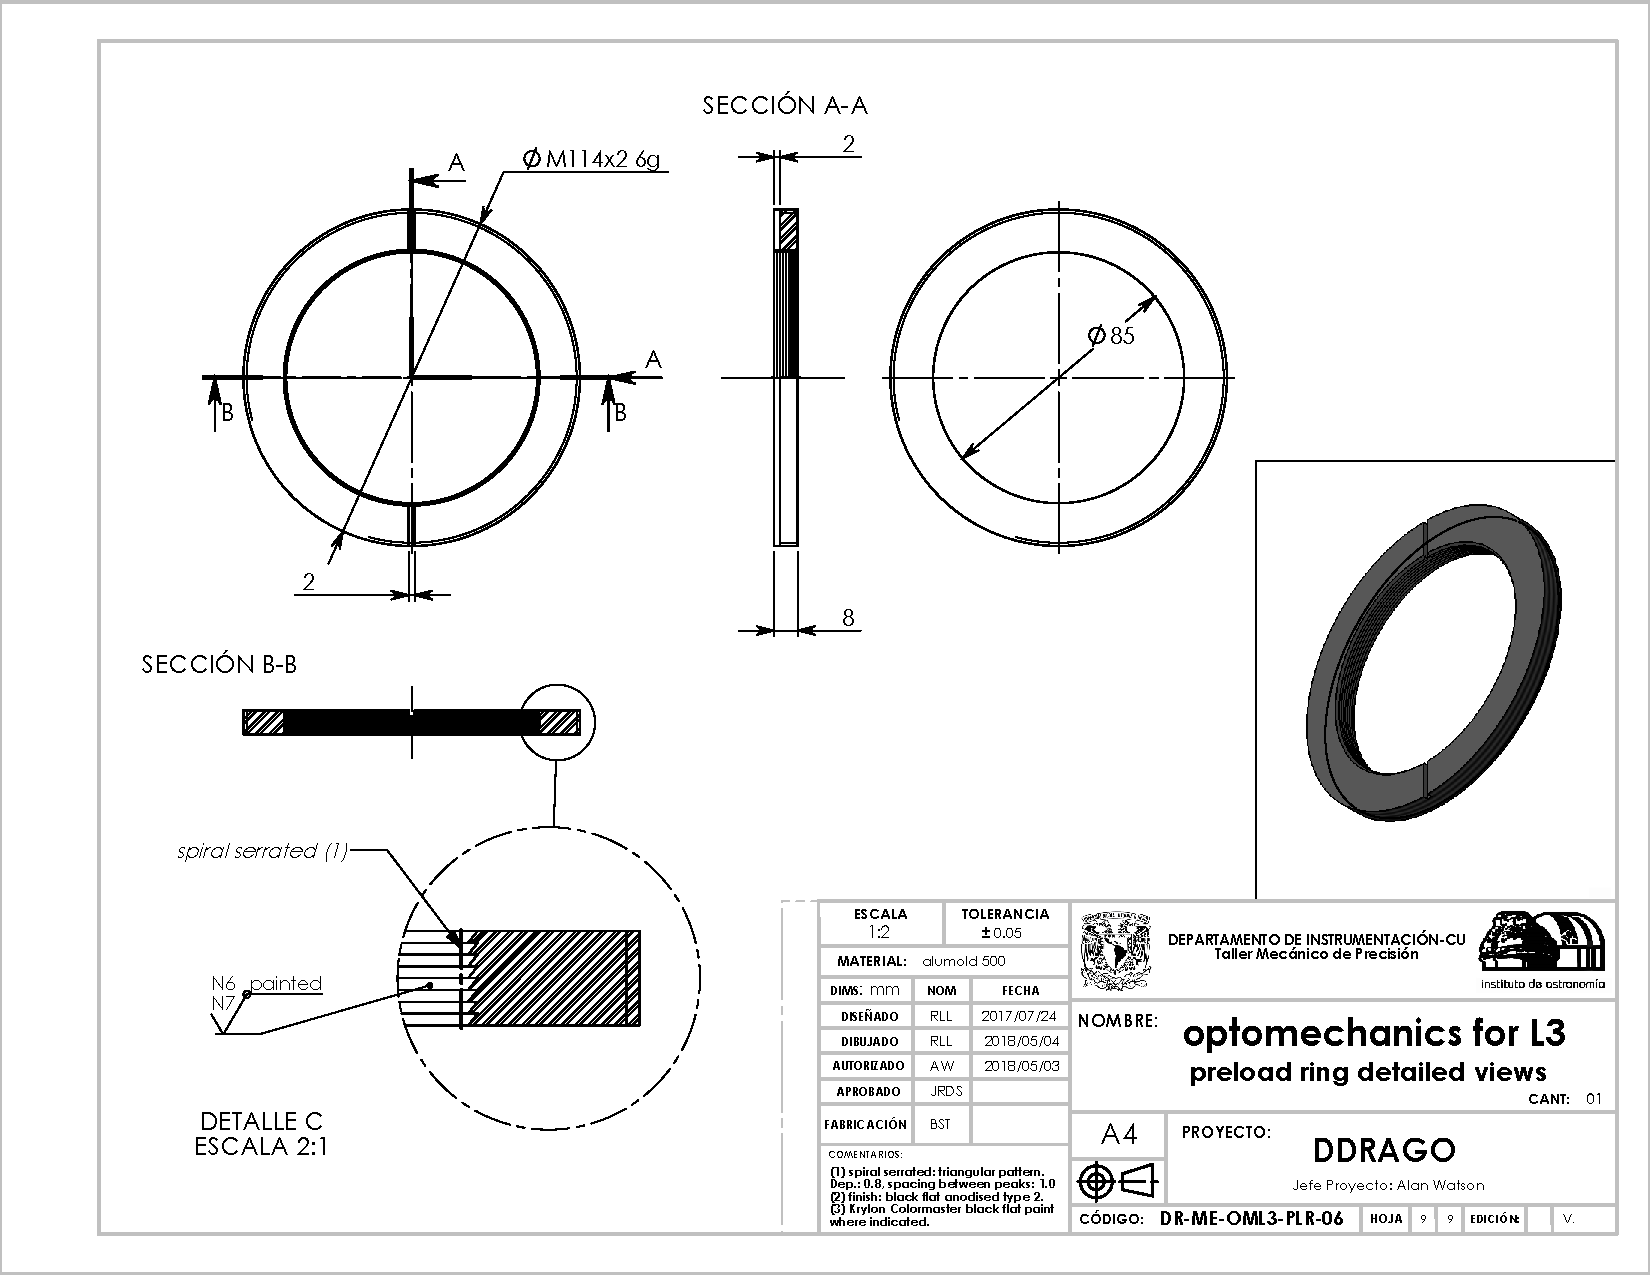
\includegraphics[height=\linewidth,angle=90]{figures/DR-ME-OML3-PLR-06}
\end{center}
\caption{The DR-ME-OML3 Barrel for L3: The DR-ME-OML3-PLR Preload Ring}
\label{figure:rosalia-oml3-plr}
\end{figure}

\begin{figure}
\begin{center}
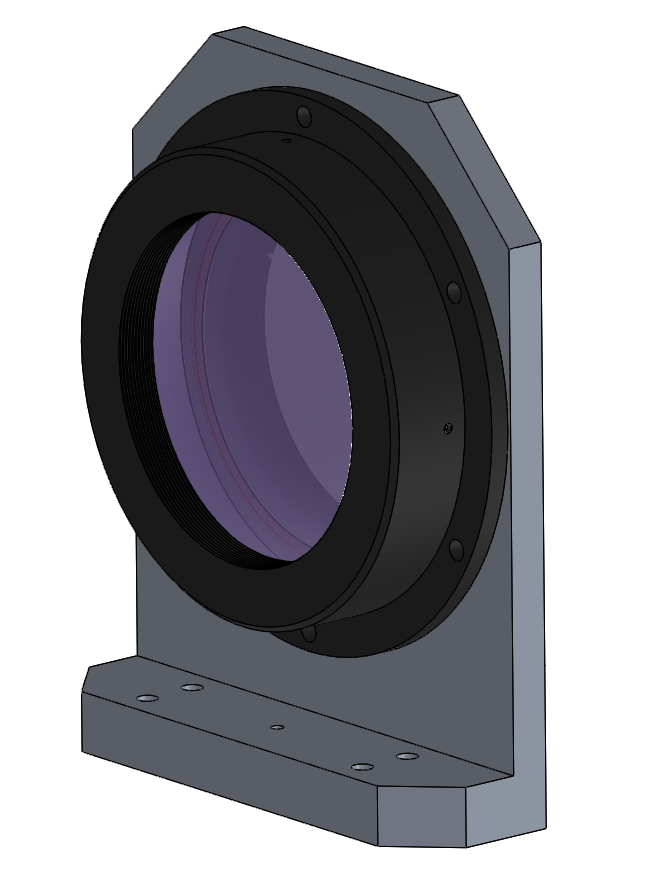
\includegraphics[width=0.7\linewidth]{newfigures/OML3.png}
\end{center}
\caption{The DR-ME-OML3-BAR Barrel Mounted on its L-Bracket DR-ME-OML3-LBR}
\label{figure:rosalia-oml3-context}
\end{figure}

L3 is a singlet meniscus lens in fused silica with a diameter of 108 mm. It constitutes the blue channel field lens. The design of the lens barrel is shown in Figures~\ref{figure:rosalia-oml3-perspective} to \ref{figure:rosalia-oml3-thermal-ring} and the individual parts in Figures~\ref{figure:rosalia-oml3-bar} to \ref{figure:rosalia-oml3-plr}. The barrel DR-ME-OML3-BAR mounts onto the L-bracket DR-ME-OML3-LBR which in turn is mounted on the plate DR-ME-IN-FP1.

The first surface of L3 is convex and with a conical shoulder that is machined in the barrel and provides tangential support. The second surface has a flat bevel in contact with its thermal ring. The cross-section diameter of this O-ring is 3.5 mm (Parker® number 2-240 S0595-50). The torque applied with its retaining ring during assembly will give the required preload and will compress the O-ring by about 20\% at maximum compression.

The barrel has threaded holes for four centering set-screws, giving $x$ and $y$ adjustments of L3. These holes are in the planes of the centre of gravity of the lens in order to have a precise control of its position.

%\subsubsection{The DR-ME-OML4 Mount for L4}
%
%\begin{figure}
%\begin{center}
%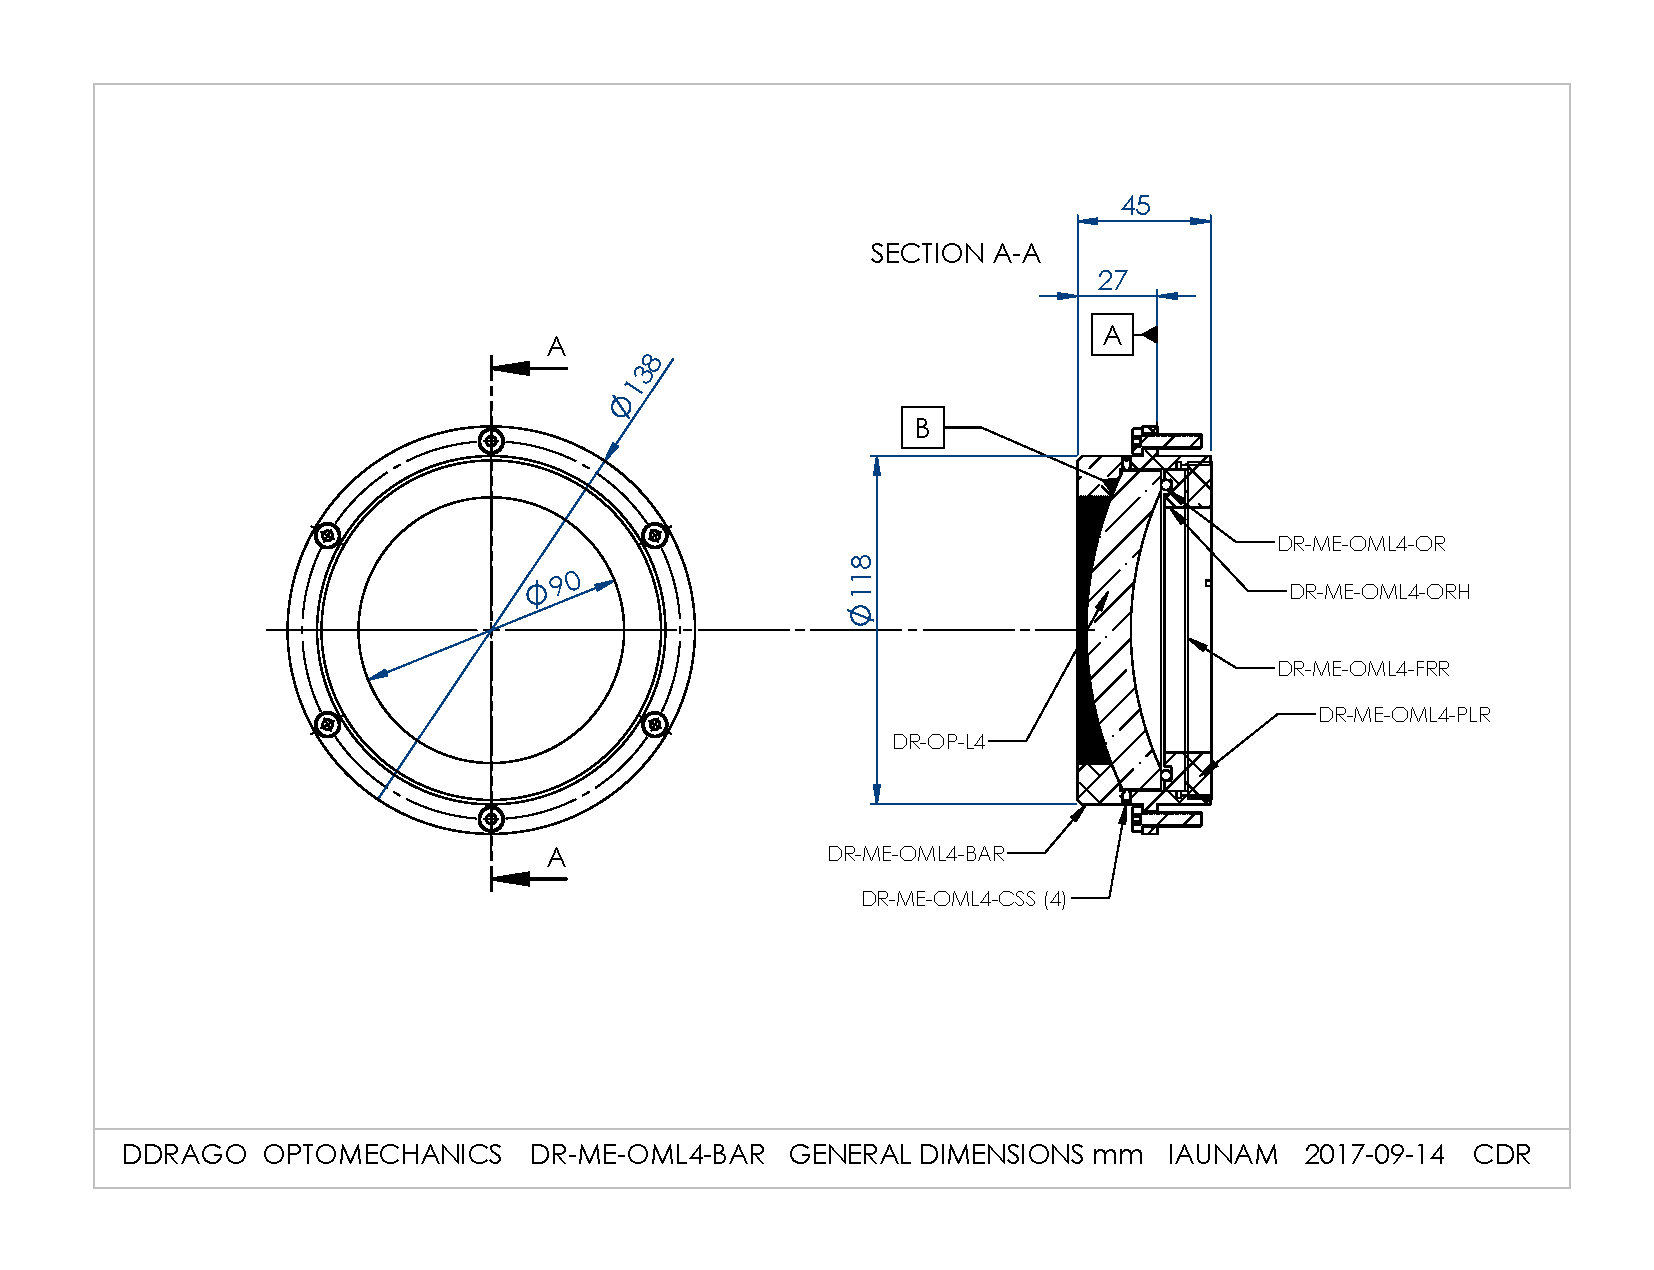
\includegraphics[height=\linewidth,angle=90]{figures/rosalia-oml4.pdf}
%\end{center}
%\caption{The DR-ME-OML4 Barrel for L4}
%\label{figure:rosalia-oml4}
%\end{figure}
%
%\begin{figure}
%\begin{center}
%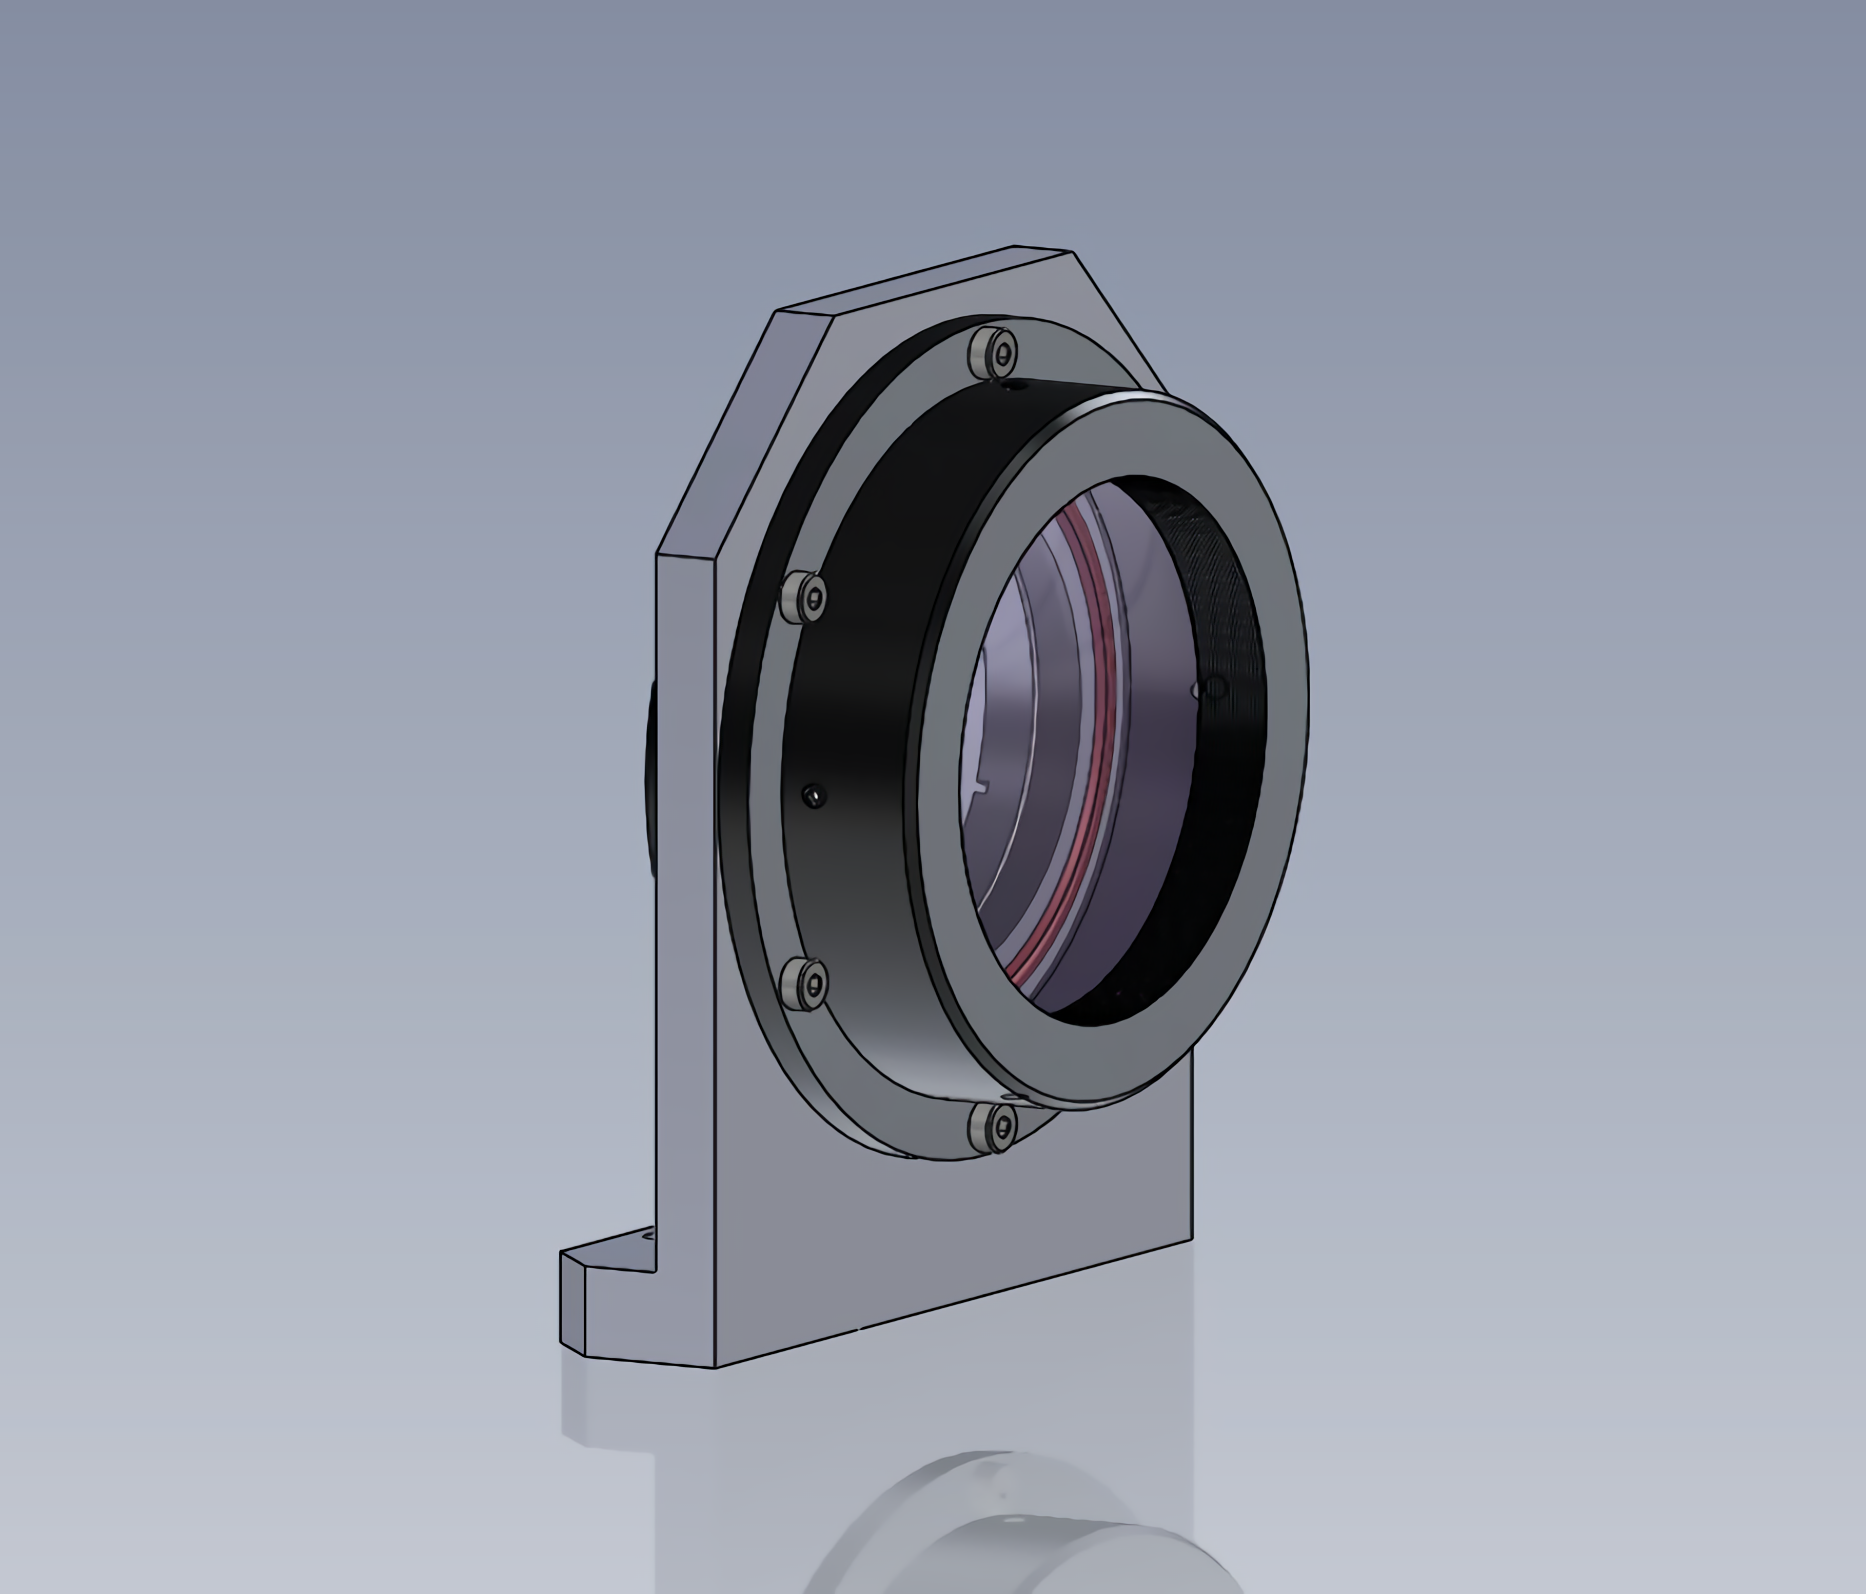
\includegraphics[width=0.7\linewidth]{figures/rosalia-oml4-context.png}
%\end{center}
%\caption{The DR-ME-OML4-BAR Barrel Mounted on its L-Bracket DR-ME-OML4-LBR}
%\label{figure:rosalia-oml4-context}
%\end{figure}
%
%\begin{figure}
%\begin{center}
%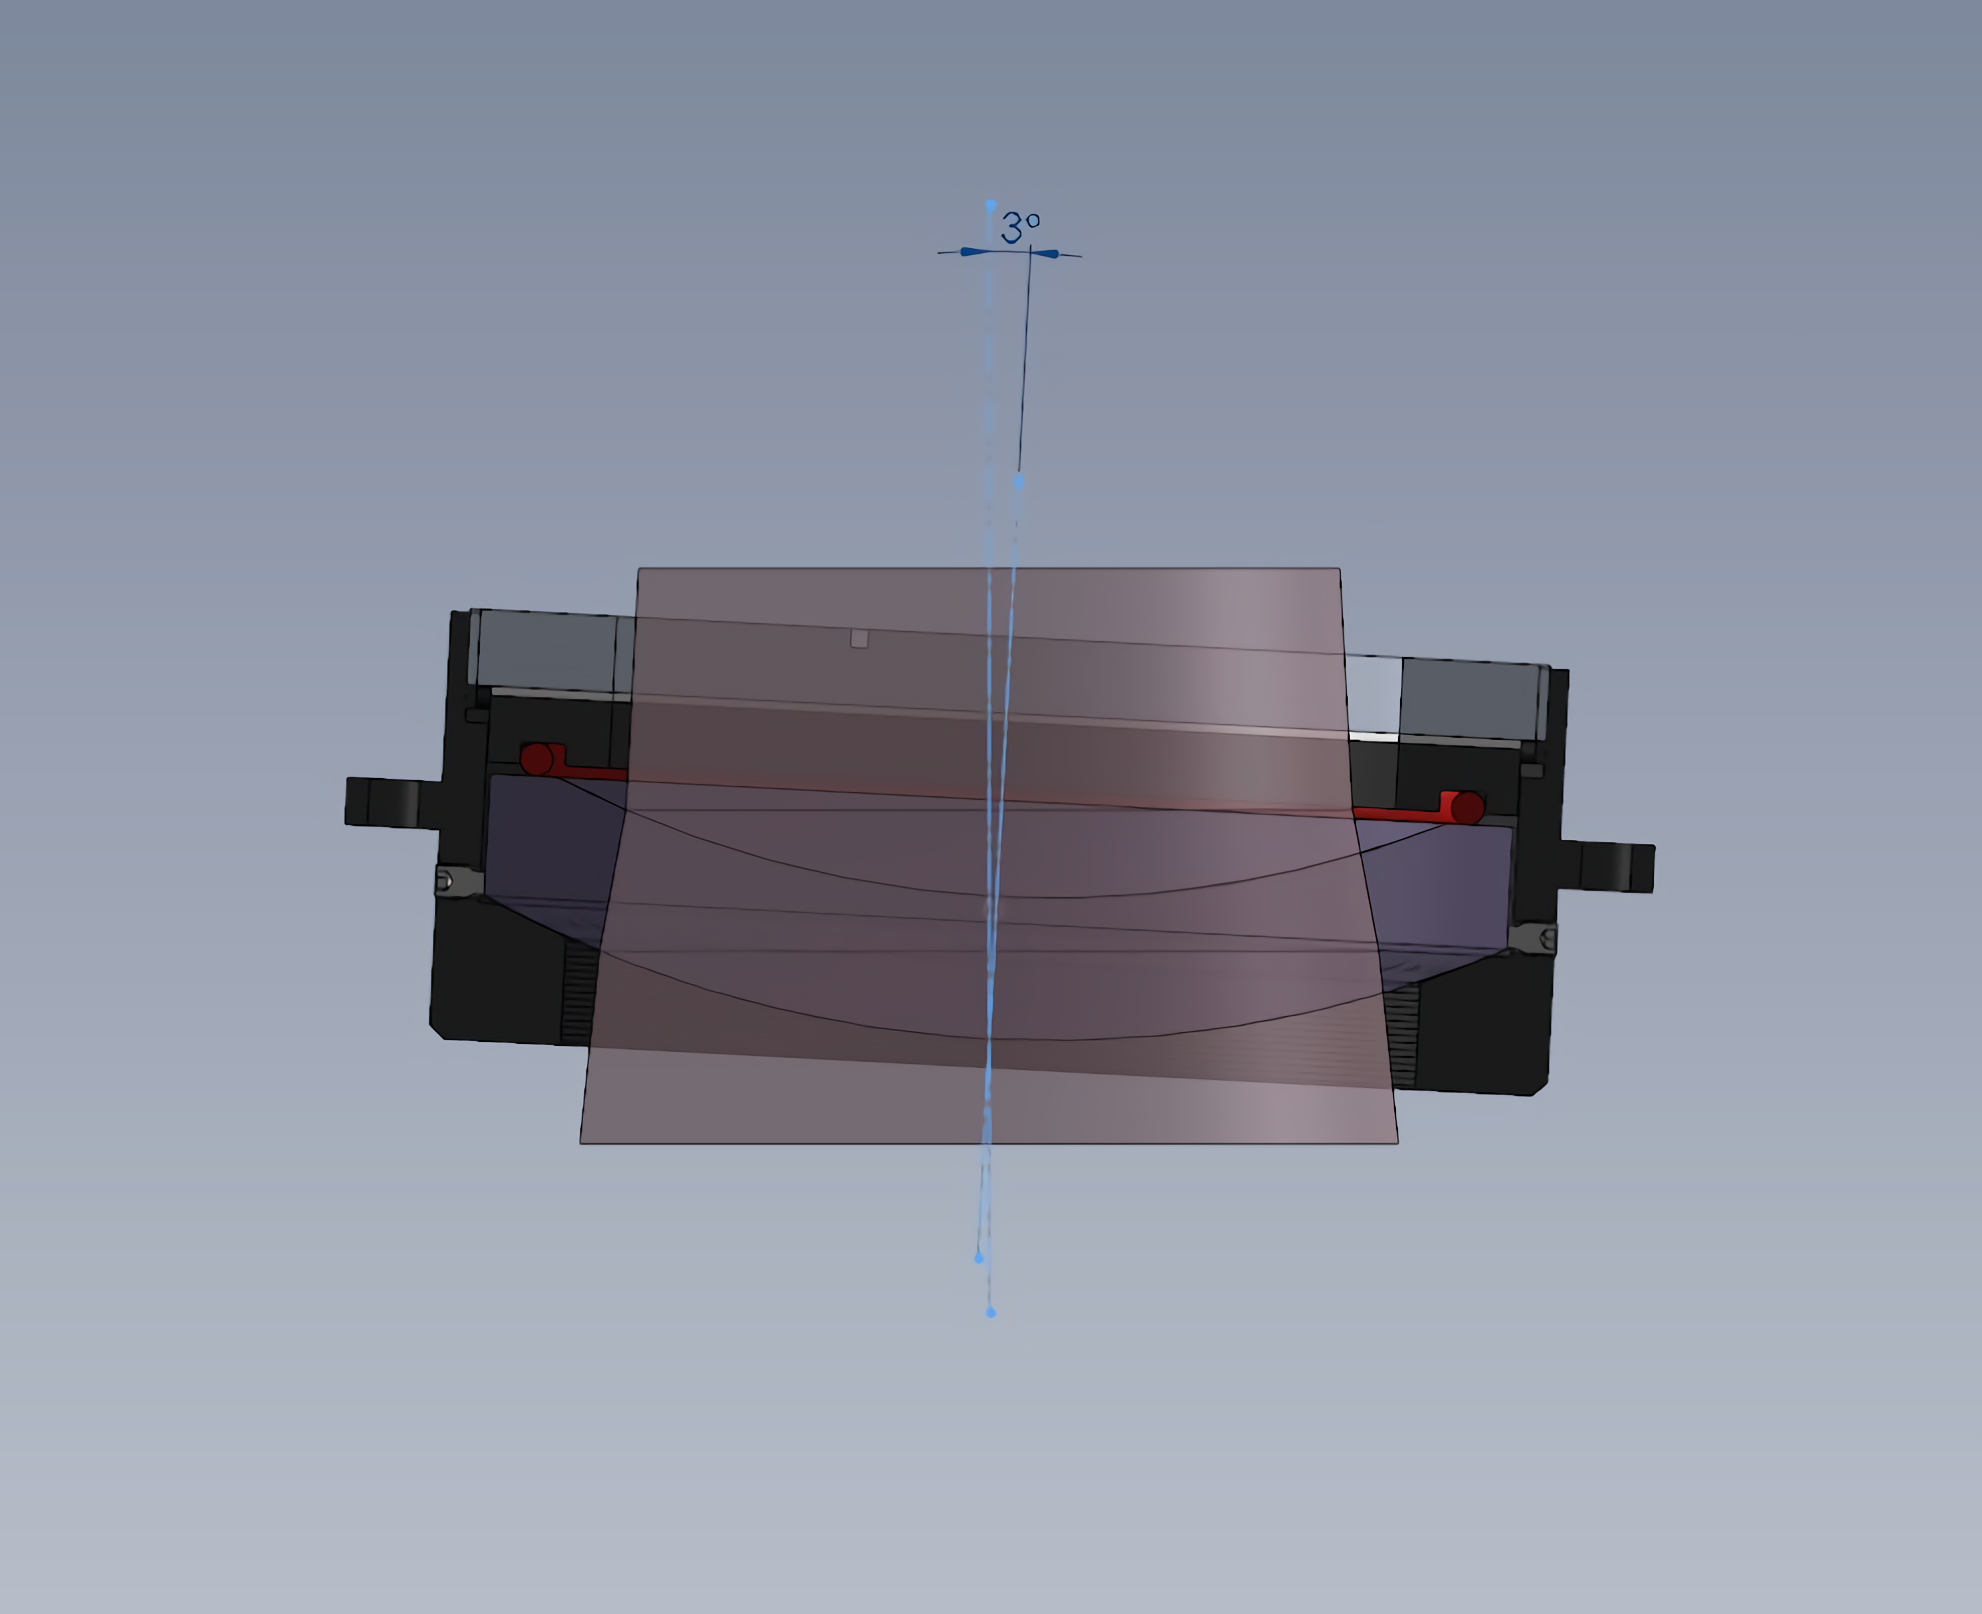
\includegraphics[width=0.7\linewidth]{figures/rosalia-oml4-tilt.png}
%\end{center}
%\caption{L4 is Tilted by the Interface between the L-Bracket DR-ME-OML4-LBR and the plate DR-ME-IN-FP1.}
%\label{figure:rosalia-oml4-tilt}
%\end{figure}
%
%L4 is a singlet meniscus lens in fused silica with a diameter of 108 mm. It constitutes the red channel field lens. The design of the lens barrel is shown in Figures~\ref{figure:rosalia-oml4} and \ref{figure:rosalia-oml4-context}.  The design of the barrel is almost the same at for L3, except that the positions of the set-screws are adjusted to match the position of the centre of gravity of L4. The barrel DR-ME-OML4-BAR mounts onto the L-bracket DR-ME-OML4-LBR which in turn is mounted on the plate DR-ME-IN-FP1.
%
%
%The first surface of L4 is convex and with a conical shoulder that is machined in the barrel and provides tangential support. The second surface has a flat bevel in contact with its thermal ring. The cross-section diameter of this O-ring is 3.5 mm (Parker® 2-240).
%The torque applied with its retaining ring during assembly will give the required preload and will compress the O-ring by about 20\% at maximum compression.
%
%The barrel has threaded holes for four centering set-screws, giving $x$ and $y$ adjustments of L4. These holes are in the planes of the centre of gravity of the lens in order to have a precise control of its position.
%
%
%The L3 and L4 barrels are similar. However, one important difference is that 
%in L4 the mechanical axis of the barrel is inclined by 3~{\deg} with respect to the optical axis of the incoming beam (to compensate the non-axisymmetric aberrations induced by transmission through D2). This requires a slightly wider inner diameter at the entrance of the barrel.
%The barrel is mounted normally in its L-bracket; the inclination of 3~{\deg} is implemented between the L-bracket and the support structure. This is shown in Figure~\ref{figure:rosalia-oml4-tilt}.

\subsection{Tolerances}

\begin{table}
\caption{Tolerances}
\label{table:tolerances}
\begin{center}
\small
\begin{tabular}{lp{2cm}p{2cm}p{6cm}}
\hline
\hline
Component&Optical\par Tolerance&Mechanical\par Tolerance&Comment\\
\hline
L1+L2	
&position\par$\pm0.2$ mm &despace\par$\pm0.05$ mm&
Length. The distance between reference surface A and entrance of barrel must have a symmetrical tolerance of ±0.05 mm.\\
&misalignment\par$\pm0.2$ mm&decenter\par$0.05$ mm&							
Concentricity. The axis of the controlled cylinder must lie within a cylindrical tolerance zone of diameter 0.05 mm and coaxial with reference.\\
&tilt\par$\pm9$ arcmin&tilt\par$0.03$ mm&
Perpendicularity. The axis of the controlled cylinder (barrel) must lie within a cylindrical tolerance zone of diameter 0.03 mm and perpendicular with reference surface A (flange).\\
\hline
L1
&position\par$\pm0.1$ mm&despace\par$\pm0.05$ mm&
Angularity. Controlled plane must lie within two parallel planes 0.05 mm apart. The angle must be theoretically exact.\\	
&misalignment\par$\pm0.3$ mm&decenter\par$0.05$ mm&
Concentricity. The axis of the controlled cylinder must lie within a cylindrical tolerance zone of diameter 0.05 mm and coaxial with reference.\\
&tilt\par$\pm6$ arcmin&tilt\par0.03 mm&Perpendicularity. The axis of the controlled cylinder (barrel) must lie within a cylindrical tolerance zone of diameter 0.03 mm and perpendicular with reference surface A (flange).\\
\hline
L2
&position\par$\pm0.2$ mm&despace\par$\pm 0.05$ mm&
Spacer length. The tolerance on the thickness or length of the spacer determines the despace tolerance of L2. This length must be theoretically exact.\\
&misalignment\par$\pm0.2$ mm&decenter\par0.05 mm&
Concentricity. The axis of the controlled cylinder must lie within a cylindrical tolerance zone of diameter 0.05 mm and coaxial with reference.\\
&tilt\par$\pm6$ arcmin&tilt\par0.05 mm&
Spacer angularity. Controlled plane in spacer must lie within two parallel planes 0.05 mm apart. The angle must be theoretically exact.\\
\hline
L3											
&position\par$\pm0.2$ mm&despace\par$\pm0.05$ mm&
Length. The distance between reference surface B and entrance of barrel must have a symmetrical tolerance of ±0.05 mm.\\
&&0.1 mm&
Angularity. Controlled plane must lie within two parallel planes 0.1 mm apart. The angle must be theoretically exact.\\
&misalignment\par$\pm1$ mm&decenter\par0.05 mm&
Concentricity. The axis of the controlled cylinder must lie within a cylindrical tolerance zone of diameter 0.05 mm and coaxial with reference.\\	
&tilt\par$\pm30$ arcmin&tilt\par0.04 mm&
Perpendicularity. The axis of the controlled cylinder (barrel) must lie within a cylindrical tolerance zone of diameter 0.04 mm and perpendicular with reference surface B (flange).\\
\hline
\end{tabular}
\end{center}
\end{table}

Table~\ref{table:tolerances} shows the translation from the optical tolerances to the mechanical tolerances for OML1L2 and OML3. The mechanical tolerances are typically much smaller than formally required by the optical tolerances but are still easily achievable. This large safety factor leaves greater margin for tolerances in the support structure and other elements.


\subsection{Manufacture}

The lens barrels, spacer, O-ring holders, and preload rings will be turned conventionally. The L-brackets will be manufactured in our CNC machine. We will use the Mitutoyo 7106 coordinate-measuring machine in the IA workshops to perform metrology the mechanical pieces. Using an iterative manufacturing process, we can typically achieve 15~{\micron} precision for the reference surfaces, which is well within the tolerances imposed by the optical design.

The friction-reducing rings will be laser-cut from 1/32-inch thick (approximately 0.8~mm) sheets.

\subsection{Centering}

\begin{table}
\caption{Self-Centerability}
\label{table:self-centerability}
\begin{center}
\small
\begin{tabular}{lccc}
\hline
\hline
Element&Karow&Hopkins&INO\\
\hline
L1&Y&N&Y\\
L2&Y&N&Y\\
L3&Y&Y&Y\\
%L4&Y&Y&Y\\
\hline
\end{tabular}
\end{center}
\end{table}

Table~\ref{table:self-centerability} shows whether each lens is self-centering according to the Karow (\ref{karow}), Hopkins (\ref{hopkins}), and INO (\ref{ino}) criteria. Each lens is self-centering according to the Karow and INO criteria but L3 is not self-centering according to the Hopkins criterion. Therefore, we feel that we cannot reply on the L3 being self-centering.

So, while we will of course take advantage of any tendency of these lenses to self-center, we will explicitly center the lenses in our ALBATROS alignment bench (see \ref{aiv}) using radially directed nylon-tipped set-screws as a temporarily aid to center the lens in its barrel. This allows us to center the lenses to better than 16~{\micron}. 

Once the lens is aligned, the assembly preload (see below) will be applied by means of a threaded preload ring until it reaches the required torque. This preload maintains the alignment.

After the preload is applied, the set-screws are backed off. (The lens barrel contracts more than the lenses at temperatures below the assembly temperature. If the set-screws are not backed off, this can cause a dangerously high stress on the lens.)

\subsection{Preload}

The lenses must be supported against axial and radial accelerations of up to $10g$. Ultimately, this support is provided by the axial preload modified by the geometry of the lens contact with the barrel and rings. The axial preload is supplied by the threaded preload ring that closes the barrel.

From these requirements, the minimum preload $F_A$ is calculated (\ref{yoder15}) according to 
\begin{equation}
F_A = \left(\frac{10Mg}{\mu}\right) \cos^2\theta,
\end{equation}
in which $M$ is the mass being supported, $g$ is the accelleration due to gravity, $\mu$ is the coefficient of static friction, and $\theta$ is the inclination of the tangential contact surface. Values of $M$, $\theta$, and $F_A$ are given in Table~\ref{table:minimum-preloads}. We assume $\mu = 0.15$ for aluminium-glass interfaces.

\begin{table}
\caption{Minimum Axial preloads}
\label{table:minimum-preloads}
\begin{center}
\small
\begin{tabular}{lllccc}
\hline
\hline
Mount&Interface&Supporting&$$M$$&$\theta$&$F_A$\\
&&&(kg)&(\deg)&(N)\\
\hline
DR-ME-OML1L2&BAR-L1&L1+SPA+L2 &3.158&\phantom{}15.1&\phantom{<}1923\\
            &L1-SPA&SPA+L2    &1.778&\phantom{0}0.0&\phantom{}<1162\\
            &SPA-L2&L2        &1.533&\phantom{}15.3&\phantom{<0}932\\
\hline
DR-ME-OML3  &BAR-L3&L3        &0.305&\phantom{}24.0&\phantom{<0}166\\
%\hline
%DR-ME-OML4  &BAR-L4&L4        &0.304&\phantom{}23.7&\phantom{<0}167\\
\hline
\end{tabular}
\end{center}
\end{table}

Some additional comments are warranted for L1+L2. First, the tangential contact between L1 and the barrel must support L1, the spacer SPA, and L2. Second, the contact between L1 and the spacer must support the spacer and L2. Finally, the contact between the spacer and L2 must support L2. Considering the three interfaces, the one that drives the minimum axial preload is the one between the barrel and L1, both because the supported mass is less for the other interfaces and because the $\mu$ will be larger than 0.15 for the interface between the ground bezel of L1 and SPA.

As the temperature changes, the dimensions of the components will change and  the axial preload will also change. To reduce this to an acceptable level, we use a passive thermal compensator situated between the last lens and the threaded preload ring. The thermal compensator consists of a soft silicone O-ring (OR), an aluminium holder (ORH), and a friction reducing ring cut from PTFE (Teflon®) sheet (FRR). The O-ring is in contact with a flat ground bevel of the last lens and absorbs most of the axial dimensional variation with temperature. The PTFE friction-reducing ring (FRR) reduces the friction at the interface between the O-ring holder (ORH) and the preload ring (PLR) and will reduce twisting of the O-ring when the preload is applied during assembly.

Silicone rubber was chosen for the O-rings because of its good heat resistance, good cold flexibility down to $-59$~C, good weather resistance, and resistance to microbiological growth.

The rate of change of preload with temperature has been considered by calculating the temperature sensitivity factor or $K_3$ for each configuration (\ref{yoder15}). The values of $K_3$, along with the preload at the assembly temperature and extreme survival temperatures, are shown in Table~\ref{table:preloads}. Note that the maximum preload varies only very slowly with temperature (because the silicone O-ring is an almost perfect thermal compensator), but that formally the maximum preload and hence the maximum stress will occur at the maximum survival temperature of $50$~C.


\begin{table}
\caption{Axial preloads}
\label{table:preloads}
\begin{center}
\small
\begin{tabular}{lcccc}
\hline
\hline
Mount&$K_3$&$-25$ C&20 C&50 C\\
&($\unit{N\,C^{-1}}$)&N&N&N\\
\hline
DR-ME-OML1L2   &$0.687$&\phantom{}1923&\phantom{}1954&\phantom{}1975\\
DR-ME-OML3     &$0.056$&\phantom{0}166&\phantom{0}169&\phantom{0}171\\
%DR-ME-OML4     &$0.056$&\phantom{0}125&\phantom{0}128&\phantom{0}129\\
\hline
\end{tabular}
\end{center}
\end{table}

At assembly, the preload will be applied by turning the preload ring to compress the O-ring. We expect the compressions to be about 30\% for L1+L2 and about 20\% for L3. However, Parker do not give sufficiently detailed information to calculate the compression with adequate precision for our purposes and it may be that the compression varies from O-ring to O-ring. Therefore, we will calibrate the relation between compression and force using an Instron compression testing machine available to us at the Faculty of Engineering of the UNAM.

Taking into account the thread of the preload ring (M185X2 for OML1L2-PLR and M114X2 for OML3-PLR) and the approximate compressions (1.06 mm for OML1L2-OR and 0.70 mm for OML3-OR), we expect to have to turn OML1L2-PLR by about 191 degrees and OML3-PLR by about 126 degrees.

The preload ring has transverse slots machined into its external face to accommodate the rectangular lugs on the end of a custom cylindrical wrench when turning the preload ring. The use of a cylindrical wrench protect the lens.

To maintain the preload, we will use a thread-locking compound (Loctite 1372603 Blue Thread Locker tape) to secure the preload ring. Using tape rather than liquid has the advantage that there is less risk of damaging a lens.

\subsection{O-Ring Compression and Set}

The preload will compress the O-rings. It is important that compression is not so much that there is contact between the lens and the O-ring holder at any temperature within the survival range.

The correct performance of DDRAGO’s thermal rings requires a continuous contact annular region
between the O-ring and the lens surface. The establishment of this annular region depends on the preload applied and the materials involved. The amount of squeeze (compression) on the O-ring should not produce an excessive deformation of the seal element. The compression load on each linear inch of an O-ring depends principally on the Shore hardness of the O-ring, its
cross-section, and the required preload. In DDRAGO’s lenses, silicone O-rings will all have a cross-section diameter of 3.53~mm (0.139~in). The L2 O-ring (with a contact circle of 168.2~mm diameter) will have a durometer of 70 Shore A and will support a
maximum axial preload at 50~C of 1975~N, which means a linear preload of 3738~N/m.
The L3 O-ring (with a contact circle of 98.4~mm diameter) will have a durometer of 50 Shore A and will support a
maximum axial preload at 50~C of 171~N, meaning a linear preload of 553~N/m.
From the Parker O-ring Handbook (\ref{parker}), Table 2-3 and Figure 2-6, it can be seen that:
L2 O-ring will have a maximum squeeze of about 30\% while L3 will have a maximum squeeze of about 20\%. These numbers were confirmed using Parker’s online “inPHorma” tool.

The maximum squeeze of 30\% on L2 O-ring means a reduction on its diameter of 1.06mm. Since the
distance between the O-ring holder and L2 is 1.53 mm, there will be a clearance of about 0.47~mm, avoiding contact between lens and O-ring holder. A maximum squeeze of 20\% on the L3 O-ring means a reduction on their diameters of 0.70 mm. Since the distance between the O-ring holders and L3 is 1.23~mm, there will be a clearance of about 0.52~mm, avoiding contact between the respective lenses and O-ring holders. Considering also the temperature dimensional changes of the O-rings, they will experience a change of $\pm0.025$~mm which is negligible here.

All the glands for DDRAGO’s O-rings have been designed following Parker recommendations, design charts and tables, with the groove outside diameter as primary and the groove inner diameter adjusted to allow a nominal gland fill of 88.56\% for L2 and 73.25\% for L3.

When under stress, rubber materials experience a progressive relaxation or creep that eventually results in a permanent deformation or “set” (\ref{parker}). The O-ring loses its O-shape causing a discontinuous contact line between the surfaces. Compression set is determined in air aging and reported by Parker as the percent of deflection by which the elastomer fails to recover after a fixed time under specified squeeze and temperature. Zero percent indicates no relaxation has occurred whereas 100\% indicates total relaxation. See Parker’s Figure 2-9 (\ref{parker}).

Failure by compression set may be caused by several conditions, the more relevant for DDRAGO case are the selection of material and seal cross-section, gland design, and temperature range.
Silicone compounds are recommended for static seals whose main requisite is to have a good (low) compression set resistance. Silicone is considered to have “G/E” (good to excellent) compression set. 

As seen in Parker’s figure 2-15 for the Silicone O-rings to be used in DDRAGO, the Compression Set is below 4\% since the maximum survival temperature is 50~C (or 122~F). With respect to temperature conditions, DDRAGO is well within the normal recommended temperature range for Silicone ($-59$~C to 204~C).

All these suggest that the selection of O-ring material, the width or cross-section, and preload applied will induce an unimportant deformation on the O-ring, that it will not fail, and that the lenses can be protected by the thermal rings.

%According to Parker® Compression Load Tables (\ref{parker}), for a 50 A Shore hardness O-ring of 3.5 mm cross section, a preload of 1622 N (maximum axial preload on L1+L2 occurring at 50~C) will induce a compression of about 35\% which means a reduction of 1.25 mm in its diameter. So, these considerations led to establish the adequate gland depth in the O-rings holders. The L2 O-ring holder is designed to leave a clearance between itself and the lens of 0.6~mm minimum at extreme conditions of preload and temperature. In the case of L3 and L4, their respective maximum preloads of 130 and 131~N will compress the O-rings by 20\% or 0.7~mm in diameter. In these cases, the minimum clearance between lens and O-ring holder is 0.5~mm.

%At assembly, the applied torque will be measured with a digital cap torque tester with a precision of ±0.5\%. 


\subsection{Compressive and Tensile Stresses}

The stresses induced within the lenses depends on the preload, the radius of the optical surfaces, the geometric shape of the mechanical interface, and the physical properties of the materials involved. 

The lenses in DDRAGO have three types of optomechanical interfaces which help to reduce contact stress: 

\begin{enumerate}
\item
Tangential interface between conical aluminium surfaces and polished convex lens surfaces (BAR-L1, SPA-L2, and BAR-L3). Since these are between two precision surfaces, the force is spread over a reasonable area of contact.
\item
Flat-bevel interface between flat aluminum surfaces and ground lens bevels (L1-SPA). Here care must be taken that the ground lens bevel is sufficiently flat to avoid restricting the contact to a few high points. This is perfectly feasible with modern grinding machines.
\item
Toroidal interface between an O-ring and ground lens bevels (L2-OR and L3-OR). Here the soft O-ring ensures that the force is spread over a reasonable area of contact.
\end{enumerate}

Compressive contact stress at these interfaces is accompanied by tensile stress occurring at the boundary of the region elastically compressed by the applied preload. The relationship between compressive stress $S_C$ and tensile stress $S_T$ is
\begin{equation}
S_T = \frac{1}{3}S_C(1-2\nu),
\end{equation}
in which $\epsilon$ is the Poisson ratio.

The maximum compressive and tensile stresses (at 50~C) are given in Table~\ref{table:stress}.

\begin{table}
\caption{Maximum Stresses (at 50 C)}
\label{table:stress}
\begin{center}
\small
\begin{tabular}{lcccc}
\hline
\hline
Lens&Material&Compressive Stress&Tensile Stress\\
&&(MPa)&(Mpa)\\
\hline
L1 &{\CaF}&9.42&1.92\\
L2 &N-BaK4&9.57&2.12\\
L3 &Fused Silica&5.87&1.70\\
%L4 &Fused Silica&&\\
\hline
\end{tabular}
\end{center}
\end{table}

\subsection{Failure Probability}

%CaF2 con St= 1.71 MPa  se tiene P(f)= 2.32X10^-9
%
%Fused Silica, con St= 1.45 MPa, se tiene P(f)= 2.61X10^-8
%
%N-BaK7  (que lo calculo como BK7), St= 1.95 MPa, se tiene P(f)< 10^-12
%
%La probabilidad de falla combinada de falla con dos lentes de Si: 5.4X10^-8
%
%Sobre el comentario de la probabilidad de falla: en efecto, casi no cambian los esfuerzos sobre las lentes (de acuerdo a la tabla 3.5). Así que estoy de acuerdo en que las lentes siempre llegan al valor del máximo esfuerzo todos los días, cuando la temperatura es máxima.
%Sean 365 noches durante 10 años de vida del instrumento son 3650 eventos. Con el valor calculado de la probabilidad de falla combinada: de 5.4X10^-8
%
%La probabilidad de al menos una falla en 10 años de vida del instrumento es de
%
%1-(1-5.4e-8)^3650 = 1.9X10^-4
%
%redondeando a 4000 eventos
%
%1-(1-5.4e-8)^4000 = 2.1X10^-4
%
%La probabilidad es despreciable (0.02%).

The probability of mechanical failure of a lens depends largely on the tensile stress. The maximum tensile stresses are shown in Table~\ref{table:stress}. Using Weibull statistics we can estimate the probability of failure when this maximum stress is applied as $5.6 \times 10^{-9}$ for the {\CaF} lens (L1), and less than $10^{-12}$ for the N-BaK4 lens (L2), and $2.4 \times 10^{-8}$ for the fused silica lens (L3).

Since the value of $K_3$ is so small, the stress on the lenses does not change dramatically from day (warmer -- higher stress) to night (colder -- lower stress). Nevertheless, we will assume that each day the lenses are taken to the maximum stress and this is then released. The probability of at least one failure when this happens is $2.4\times10^{-8}$ per day. 
The probability of at least one failure over the approximately 4000 day design lifetime of the instrument is about $1.0\times10^{-4}$. So, the probability of failure is negligible.

%\subsection{Birefringence}
%
%Surface deformation and related birefringence effects from mounting forces are in the local regions where those forces are applied. These regions are outside the optics’ clear apertures, so the effects will not be significant.
%
%\textcolor{red}{TODO: The stress on L4 is \emph{not} higher than the stress on L1 or L2. I think this calculation needs to be redone with the new stresses.}
%
%\textcolor{red}{TODO: I don’t have this figure.}
%
%As an example, the Figure XX shows the case of L4, a fused silica lens whose optical stress coefficient ($K_s=3.40 \times 10^{-6}$~\unit{Pa^{-1}} at 589.3 nm and 21 C) is higher than that for CaF2 or N-BAK4. The average compressive stress acting on this lens is also higher than on the other lenses (5.00 MPa at 20 C) and so, the optical path difference is also higher (185.35 nm).
%
%Comparing the area of contact stress into the lens with the diameter of the clear aperture, it can be seen that the latter is smaller than the stressed region, so the birefringence resulting from stress is not relevant.

%\clearpage
%\section{Dichroic and Corrector Plate Supports}
%
%\subsection{General Design}
%
%At PDR we presented a design for the optomechnical supports of the dichroics based on the design used in RATIR. This supported one surface of the dichroic at three points and used three retaining springs. However, finite-element analysis of this design showed that this design produced excessive distortions in the larger dichroics used in DDRAGO.
%
%\begin{figure}[p]
%\begin{center}
%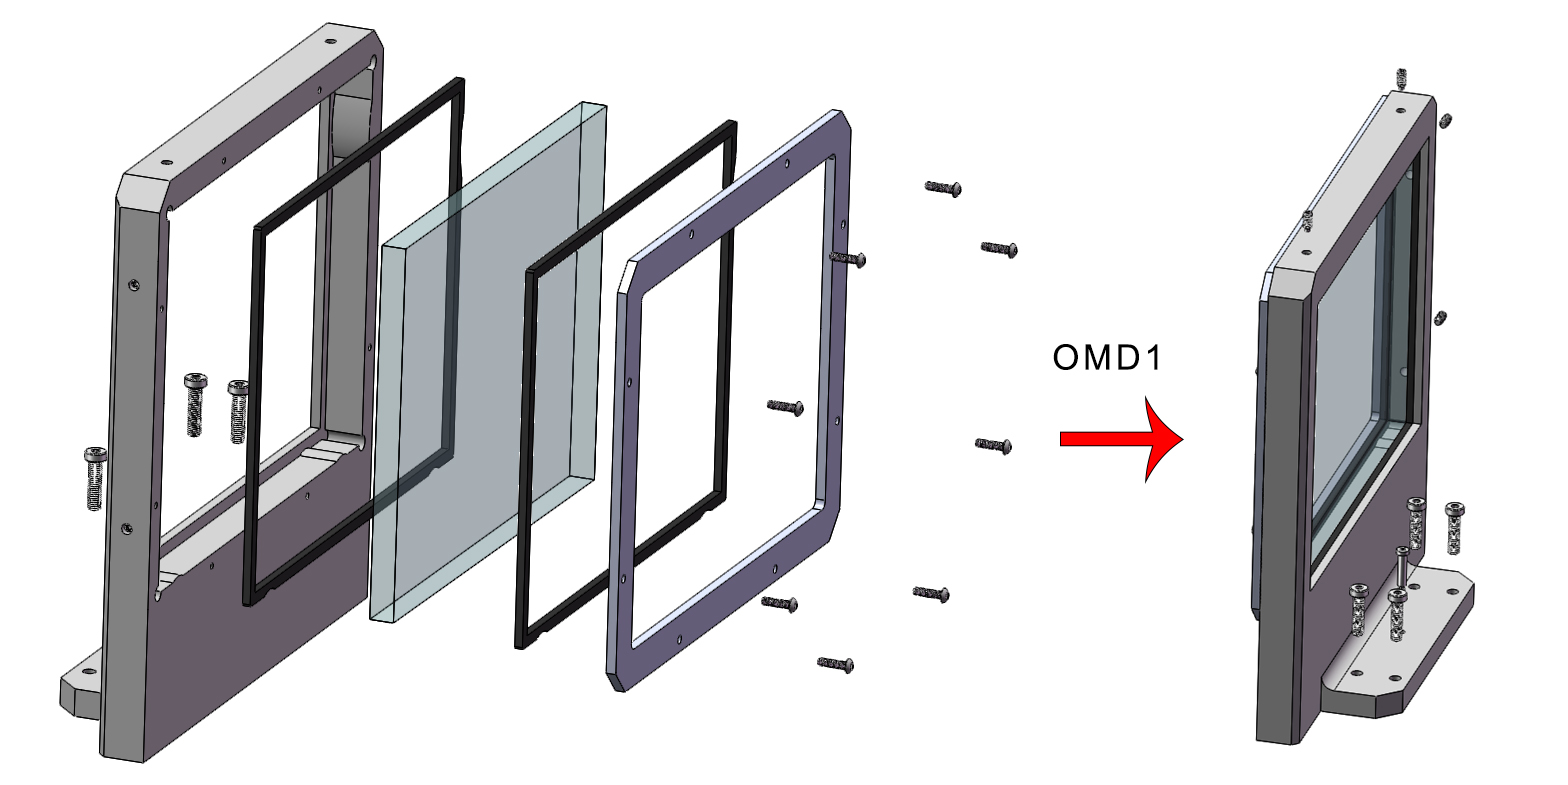
\includegraphics[width=\linewidth]{figures/alex-omd1.jpg}
%\end{center}
%\caption{The DR-ME-OMD1 Support for D1.}
%\label{figure:alex-omd1}
%\end{figure}
%
%We therefore changed the design to support the dichroics along their complete circumference between two 3.175~mm (1/8 inch) cushions of black FPM fluoroelastomer. The specific product we use is Dupont Viton® (McMaster-Carr part number 86075K34). The basic design is shown for the optomechanical support OMD1 for D1 in Figure~\ref{figure:alex-omd1}. In this design, the L-bracket OMD1-LBR has a pocket. This pocket holds the first FPM cushion OMD1-CSH1, the dichroic D1, and the second FPM cushion OMD1-CSH2. The pocket is closed by an aluminum cover OMD1-CVR. Note that the dichroics are wedged, so the cover will not close parallel to the surface of the L-bracket but will be slightly inclined. Lateral support is supplied by three reference surfaces on the inside of the pocket and four nylon-tipped set-screws.
%
%\TODO{OMCP in the STEP file uses the old design. This needs updating.}
%
%\TODO{Update to use two shoulder bolts, since we no longer need tilt adjustment.}
%
%The designs of the supports OMD2 for D2 and OMCP for CP are similar.
%
%\begin{table}[p]
%\caption{Extract of the Product Tree Table Relevant for the Dichroic and Corrector Plate Mounts}
%\label{table:dichroic-product-tree}
%\begin{center}
%\small
%\begin{tabular}{ll}
%\hline
%\hline
%Code                &Description\\
%\hline
%DR-ME-OMD1          &Optomechanics for D1\\
%DR-ME-OMD1-LBR      &L-Bracket\\
%DR-ME-OMD1-CSH1     &Cushion 1\\
%DR-OP-D1            &Dichroic D1\\
%DR-ME-OMD1-CSH2     &Cushion 2\\
%DR-ME-OMD1-CVR      &Cover\\
%\hline
%DR-ME-OMD2          &Optomechanics for D2\\
%DR-ME-OMD2-LBR      &L-Bracket\\
%DR-ME-OMD2-CSH1     &Cushion 1\\
%DR-OP-D2            &Dichroic D2\\
%DR-ME-OMD2-CSH2     &Cushion 2\\
%DR-ME-OMD2-CVR      &Cover\\
%\hline
%DR-ME-OMCP          &Optomechanics for CP\\
%DR-ME-OMCP-LBR      &L-Bracket\\
%DR-ME-OMCP-CSH1     &Cushion 1\\
%DR-OP-CP            &Corrector Plate CP\\
%DR-ME-OMCP-CSH2     &Cushion 2\\
%DR-ME-OMCP-CVR      &Cover\\
%\hline
%\end{tabular}
%\end{center}
%\end{table}
%
%Table~\ref{table:dichroic-product-tree} shows an extract of the product tree table relevant for the dichroic and corrector plate mounts.
%
%The L-brackets are attached to the corresponding plates of the support structure using bolts for strength and smaller shoulder bolts to achieve their required tolerances by manufacture.
%
%The design uses Alumold 500 (although an equivalent 7000-series alloy could be substituted if need be). Alumold 500 is suitable for precision machining.
%
%\subsection{Manufacture}
%
%We will manufacture the aluminum parts for OMD1, OMD2, and OMCP in our CNC machine.
%
%We will cut the FPM cushions from 3.175~mm (1/8~inch) sheet using a knife. We prefer not to use our laser cutter, since it can cause heat damage to the bulk of the material and leave an unacceptably rough edge.
%
%\subsection{Distortion and Displacement}
%
%\TODO{5~nm seems too small. Check this.}
%
%Figure~\ref{figure:alex-d1-fea} shows the distortion and displacement of D1 under a gravity vector perpendicular to its surface. The displacement of the dichroic is about 5~{\micron} and the distortion about 5~nm, both of which are negligible in terms of the tolerances on these from the optical design. Since D2 and CP are smaller, the displacements and distortions will even smaller.
%
%\begin{figure}
%\begin{center}
%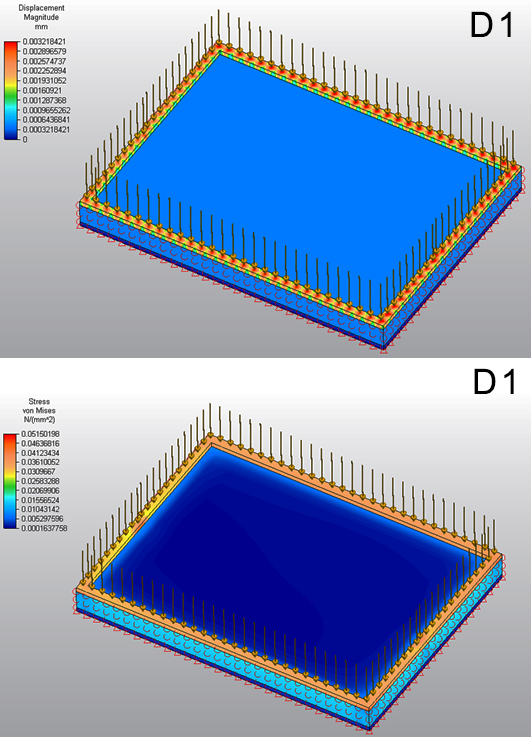
\includegraphics[width=\linewidth]{figures/alex-d1-fea.jpg}
%\end{center}
%\caption{The Support for D2}
%\label{figure:alex-d1-fea}
%\end{figure}

\clearpage
\section{DDRAGO Detector Supports}

\begin{figure}[p]
\begin{center}
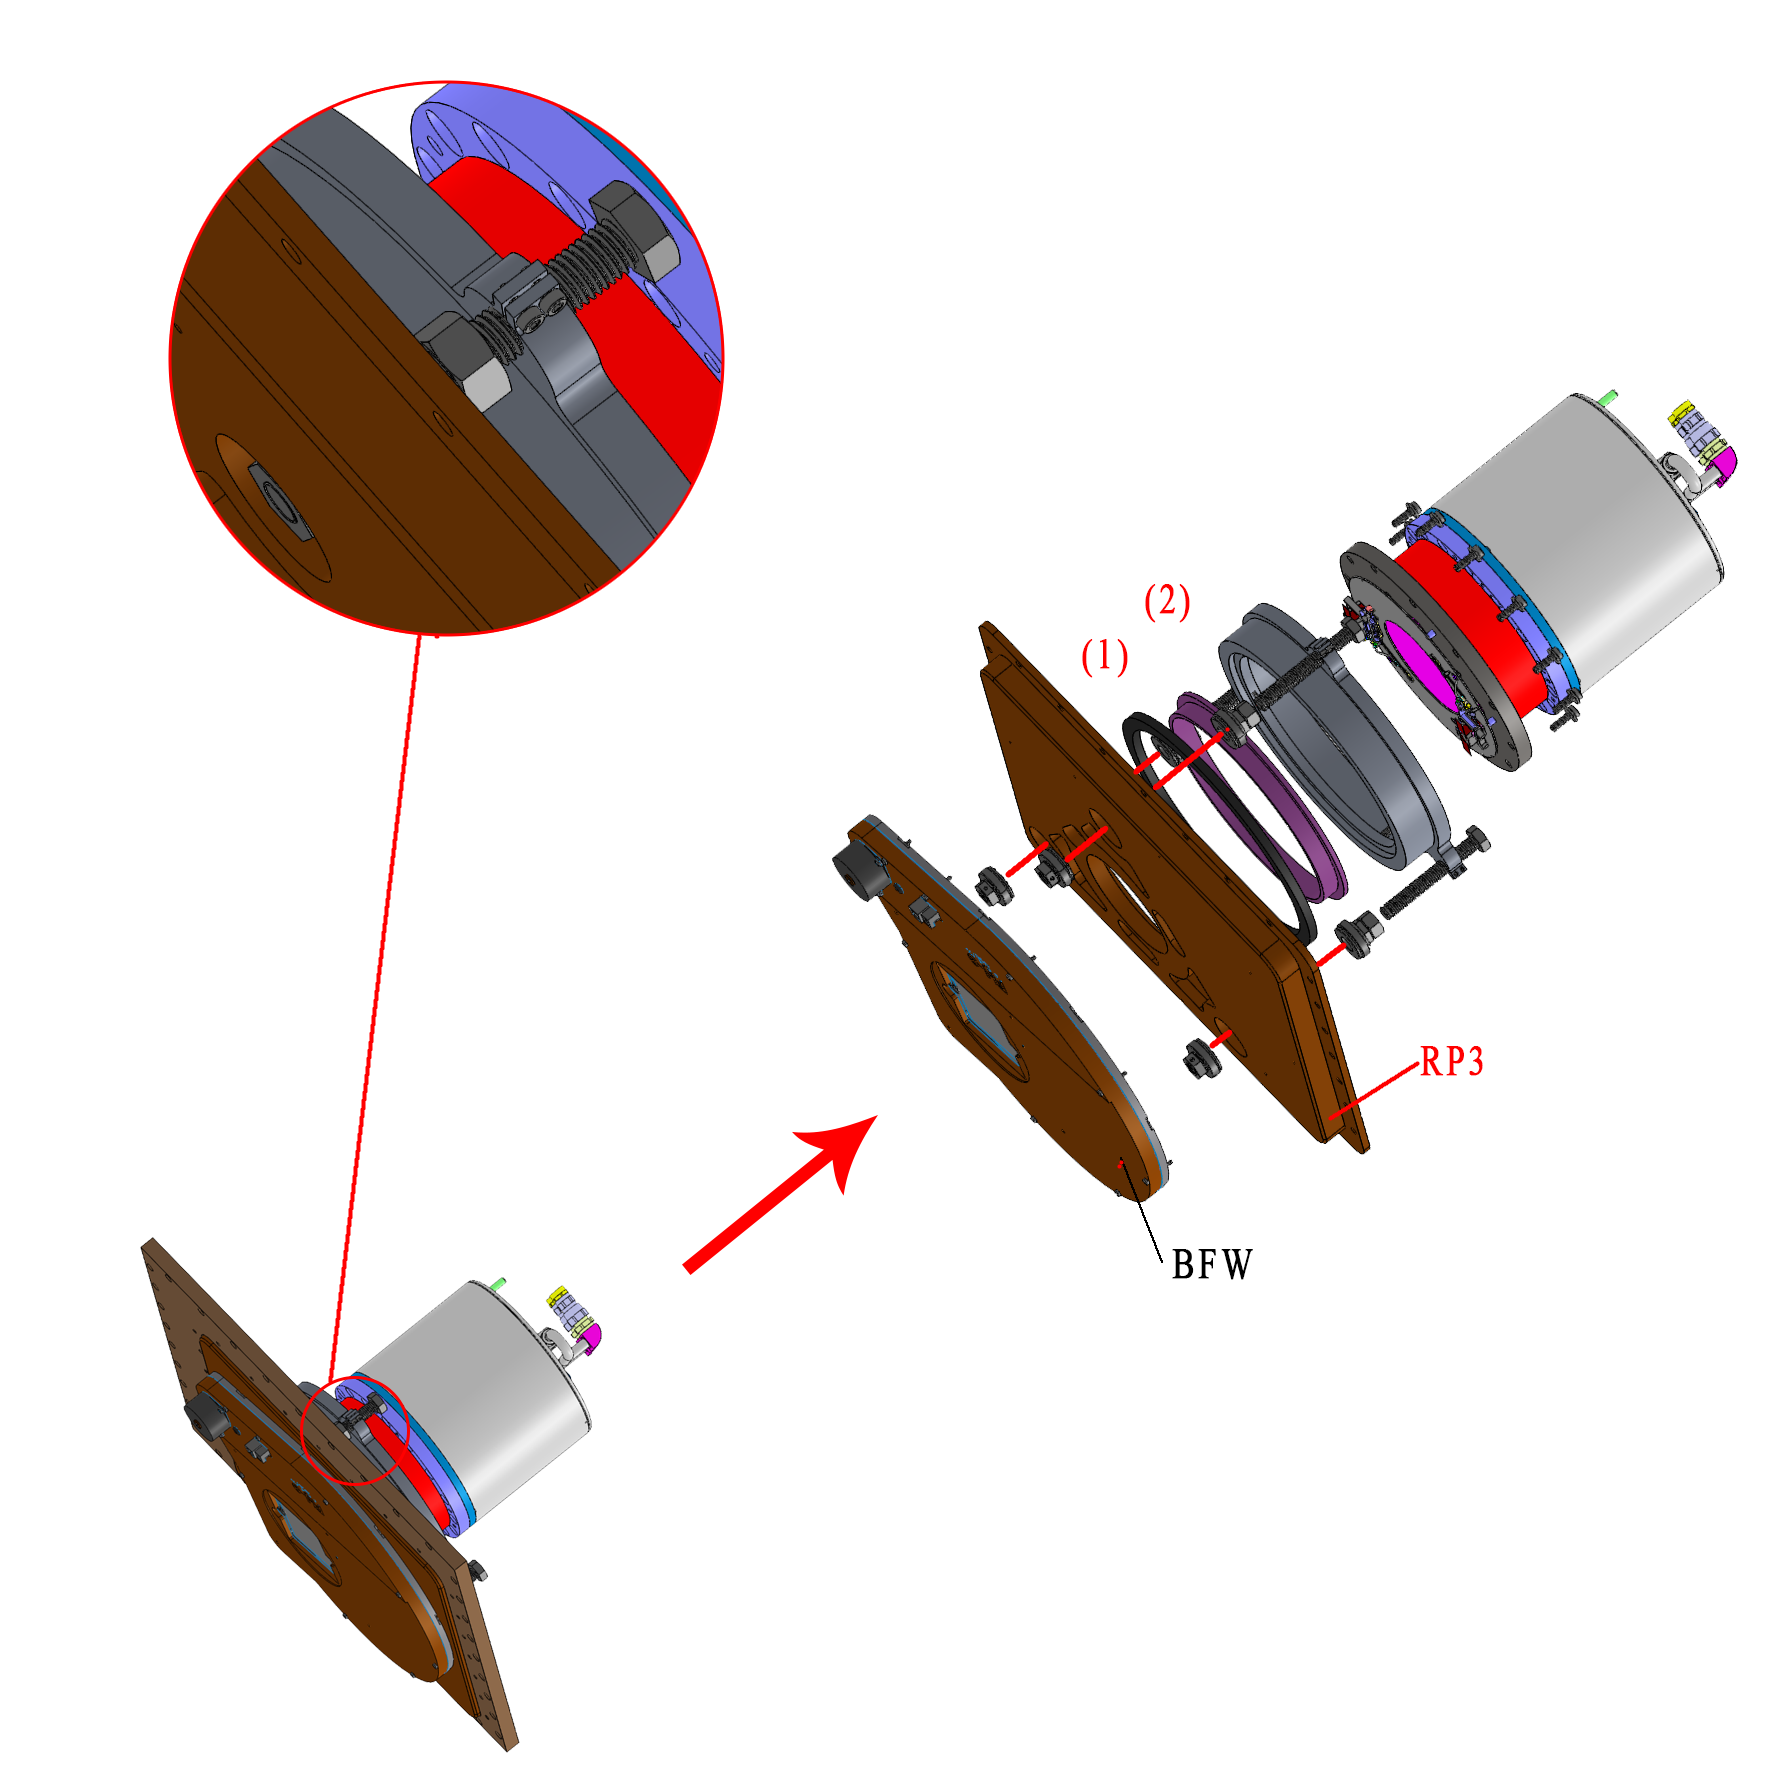
\includegraphics[width=\linewidth]{newfigures/Fig5_1.png}
\end{center}
\caption{The Detector Mount.}
\label{figure:alex-detector-mount}
\end{figure}

\subsection{Design}

We need to be able to statically adjust the detector in focus and tilt.

At PDR, we proposed to do this by shimming. This is extremely laborious. 

We now propose to adopt a design that we have used successfully to adjust the tilt of the detectors in the DDOTI project. The design is shown in Figure~\ref{figure:alex-detector-mount}. It uses three M12 bolts to acting between an adapter ring (which is attached to the detector head) and a support structure removable plate. The attachment to the support structure uses spherical washers to allow the bolts to tilt as well as extend.

Normally, the play in the bolt thread would limit the precision with which we could position the detector. To counteract this, after adjustment, the threads in the adapter ring are tightened on the M12 bolt using two lateral tightening bolts (see in (b) of Figure~\ref{figure:alex-detector-mount}). We have verified that this reduces the play to about 5~{\micron}, which is now negligible. The play between the M12 bolt and the removable plate is also eliminated by the use of locking nuts on both sides of the spherical washers.

The gap between the adapter ring and the removable plate is sealed against light in two ways. First, the adapter ring has an extension into the removable plate, which acts as a baffle. Second, we will place a compressible black EVA foam liner cut from 3/8-inch thick sheet (McMaster part 86095K43) between the ring and the plate.

The design uses Alumold 500 (although an equivalent 7000-series alloy could be substituted if need be). Alumold 500 is suitable for precision machining.

\subsection{Manufacture}

We will manufacture the aluminum parts in our CNC machine.

%\clearpage
%\section{CAGIRE WOB Masks}
%
%The CAGIRE WOB will be aligned using a set of masks, one in the focal plane before L5 and the other just before L8. In operation, the L5 mask will be replaced with a field mask to reduce scattered light. These mask holders are shown in Figure~\ref{figure:alex-M1}.
%
%\begin{figure}[p]
%\begin{center}
%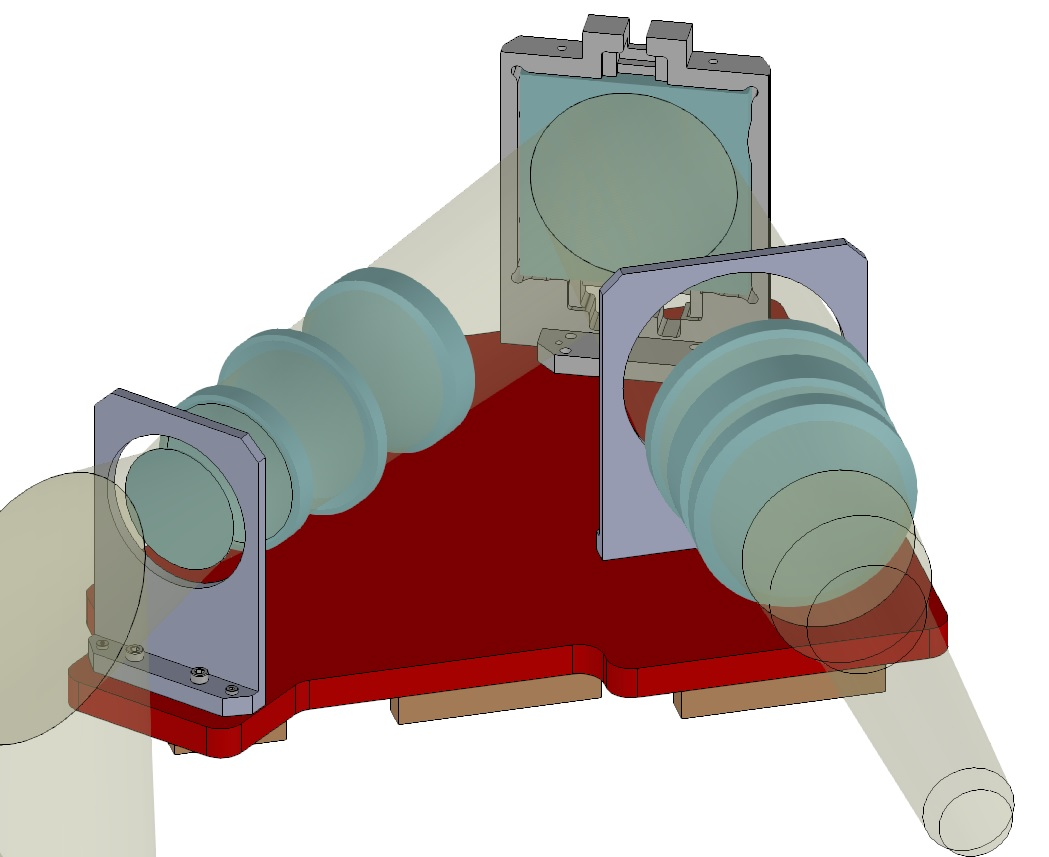
\includegraphics[width=\linewidth]{figures/alex-M1.jpg}
%\end{center}
%\caption{The Mask Supports on the CAGIRE WOB}
%\label{figure:alex-M1}
%\end{figure}

\clearpage
\section{Mechanisms}

\subsection{Shutter}

The DDRAGO CCD has an integrated Vincent/Uniblitz CS90 shutters.

\subsection{Filter Wheel}

\begin{figure}[p]
\begin{center}
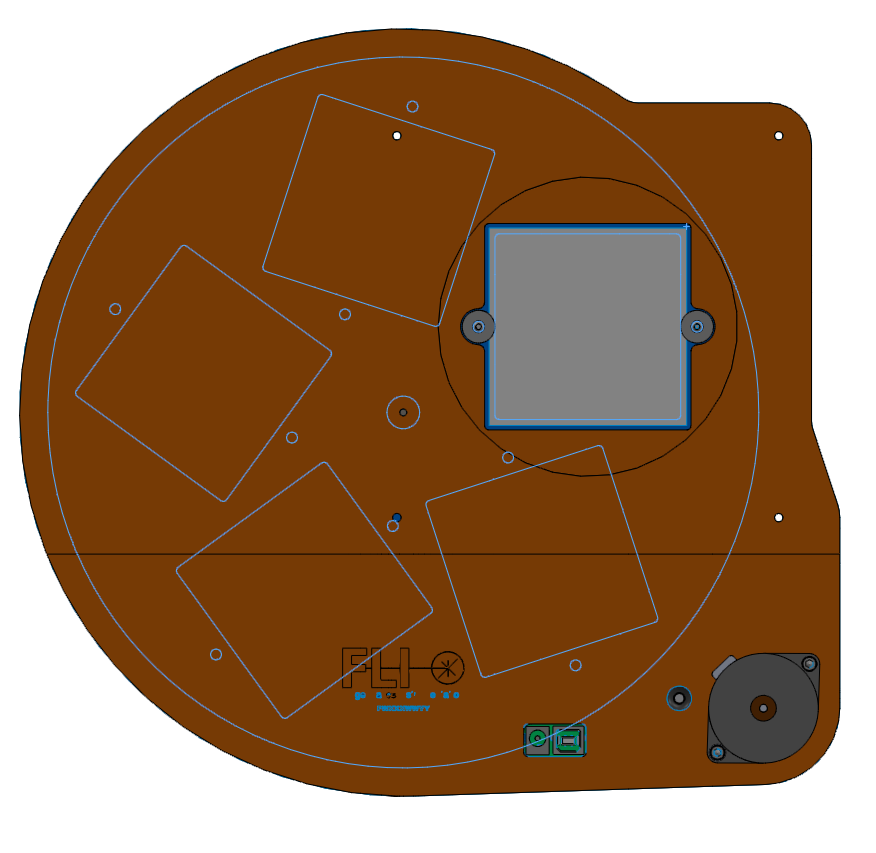
\includegraphics[width=\linewidth]{newfigures/Fig6_1.png}
\end{center}
\caption{The DDRAGO FLI CFW-14-5 Filter Wheels.}
\label{figure:alex-ddrago-cfw}
\end{figure}

The interim imager will use a FLI CFW-14-5 filter wheel. These have been customized by FLI to accept five 76 mm square filters (see Figure~\ref{figure:alex-ddrago-cfw}). We have three examples: one for the interim instrument or the blue channel of the definitive instrument, one for the red channel of the definitive instrument, and one spare.

We will perforate the wall of the filter wheel to allow it to be mounted to the support structure. We have experience mounting a similar filter wheel this way in the COATLI interim instrument. Unfortunately, the position of the connectors forces the cover of the filter wheel to be against the support structure plate RP5. This means that changing filters requires removing the whole filter wheel. That said, we do not expect to change filters frequently.

%\subsection{CAGIRE Filter Wheel}
%
%\begin{figure}
%\begin{center}
%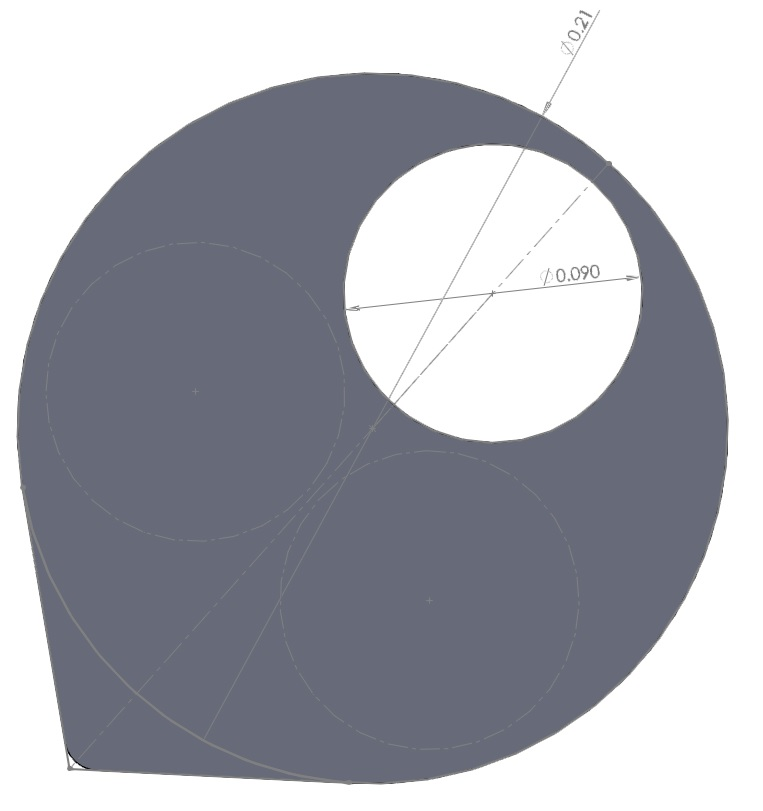
\includegraphics[width=\linewidth]{figures/alex-cagire-cfw.jpg}
%\end{center}
%\caption{A Suggested CAGIRE FLI CFW-2 Filter Wheel.}
%\label{figure:alex-cagire-cfw}
%\end{figure}
%
%Our current interface agreement with the IRAP has the custom CAGIRE filter wheel outside of the support structure. Thus, the interface is between the support structure on one hand and the filter wheel and cryostat on the other. We consider that complicates the implementation of the interface.
%
%Instead, we would suggest that CAGIRE uses a modified FLI filter wheel, similar to the ones used by DDRAGO. Figure~\ref{figure:alex-cagire-cfw}
% shows that three round 90-mm filters ($J$, $\Hs$, and reflective) can fit in a modified CFW-2 wheel. This wheel could then be mounted to an inside wall of the support structure wall in the same way that the DDRAGO wheels are mounted to inside walls. The cryostat could then mount to the corresponding outside wall.
%
%FLI have offered to produce three modified filter wheels for DDRAGO (two for use and one spare) for US\$18,750 with less than 9 months delivery time. We would imagine the cost and delivery time for two or three modified filter wheels for CAGIRE would be similar.

%\subsection{CAGIRE Focuser Stage}
%
%We propose to focus CAGIRE by moving the L7 lens with an FLI Atlas focuser. 
%
%Our current design has the Atlas focuser after L7 and separated from the L5+L6 barrel (see Figure~\ref{figure:alex-OB1}). This makes alignment of the L5+L6+L7 triplet in the ALBATROS bench rather difficult. In the detailed design, we may place the Atlas before L7 and mount it to the L5+L6 barrel. Alternatively, we may mount the L5+L6 barrel and the Atlas+L7 separately on a common structure and then mount the common structure on the WOB. Either of these options would facilitate alignment.
%
%The mechanical performance of the Atlas focuser  will be verified experimentally at the laboratory shortly after PDR.
%
%\begin{figure}
%\begin{center}
%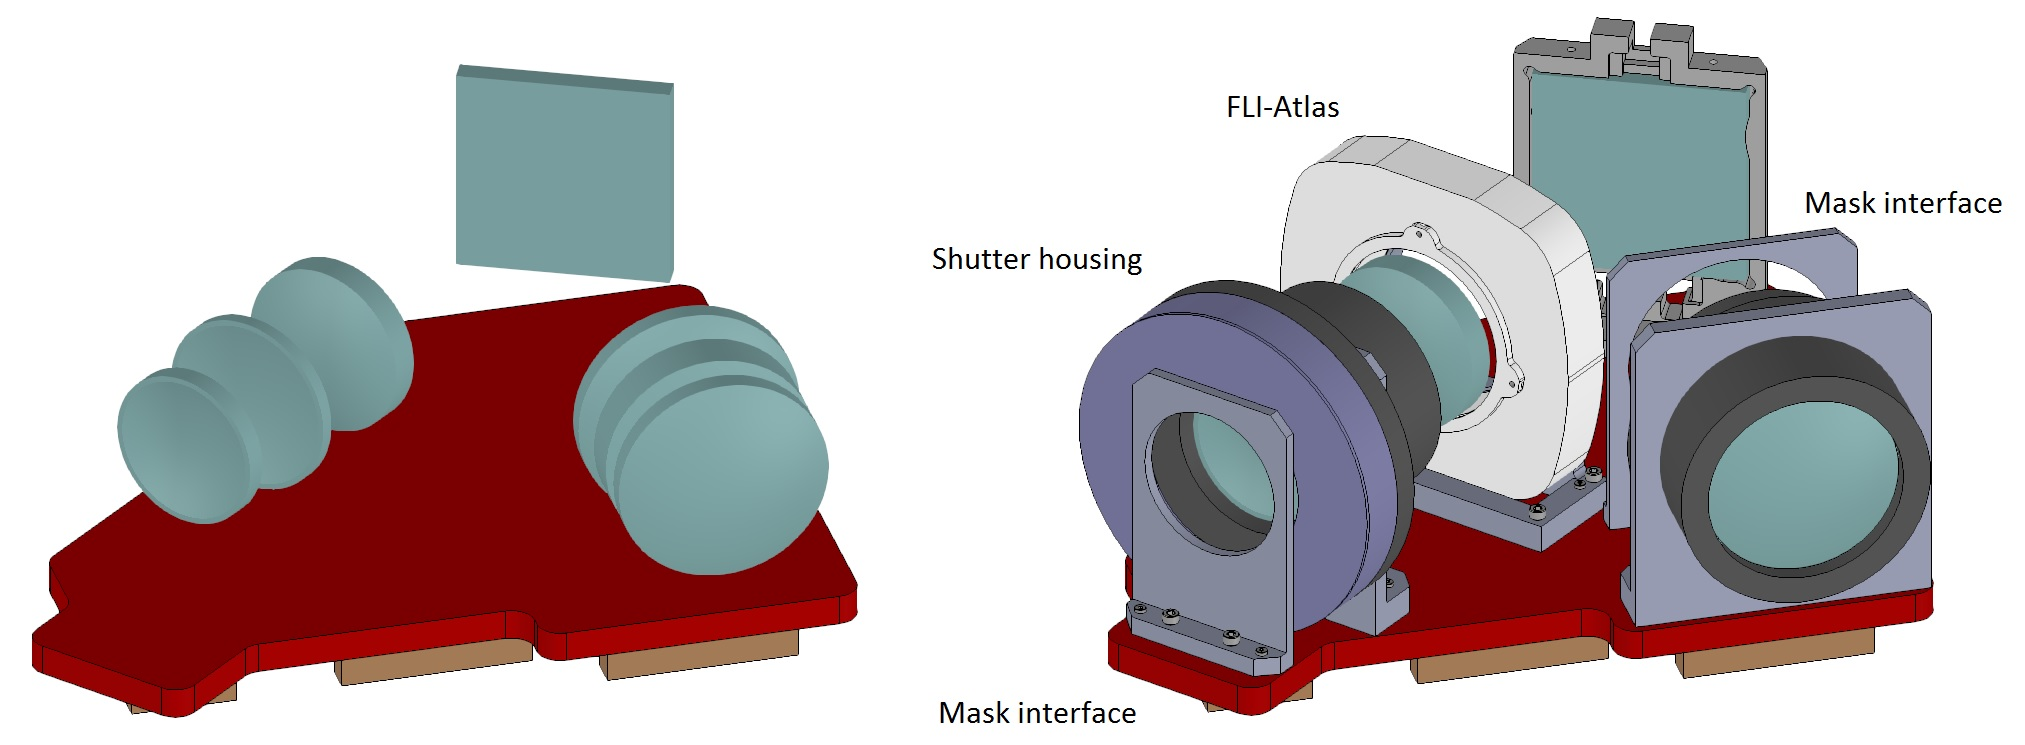
\includegraphics[width=\linewidth]{figures/alex-OB1.jpg}
%\end{center}
%\caption{The Atlas Focuser on the CAGIRE WOB.}
%\label{figure:alex-OB1}
%\end{figure}
%
%\subsection{CAGIRE Shutter}
%
%The FPRD requires a mechanical shutter for CAGIRE. We propose to place it before L5, where the beam is relatively compact. Even so, the beam is slightly too large for a 65~mm shutter. Therefore, we will use the same model of 90~mm Vincent/Uniblitz CS90 shutter used in the CCDs. Figure~\ref{figure:alex-S1} shows the shutter and the way it could be attached to the L5+L6 lens barrel.
%
%\begin{figure}
%\begin{center}
%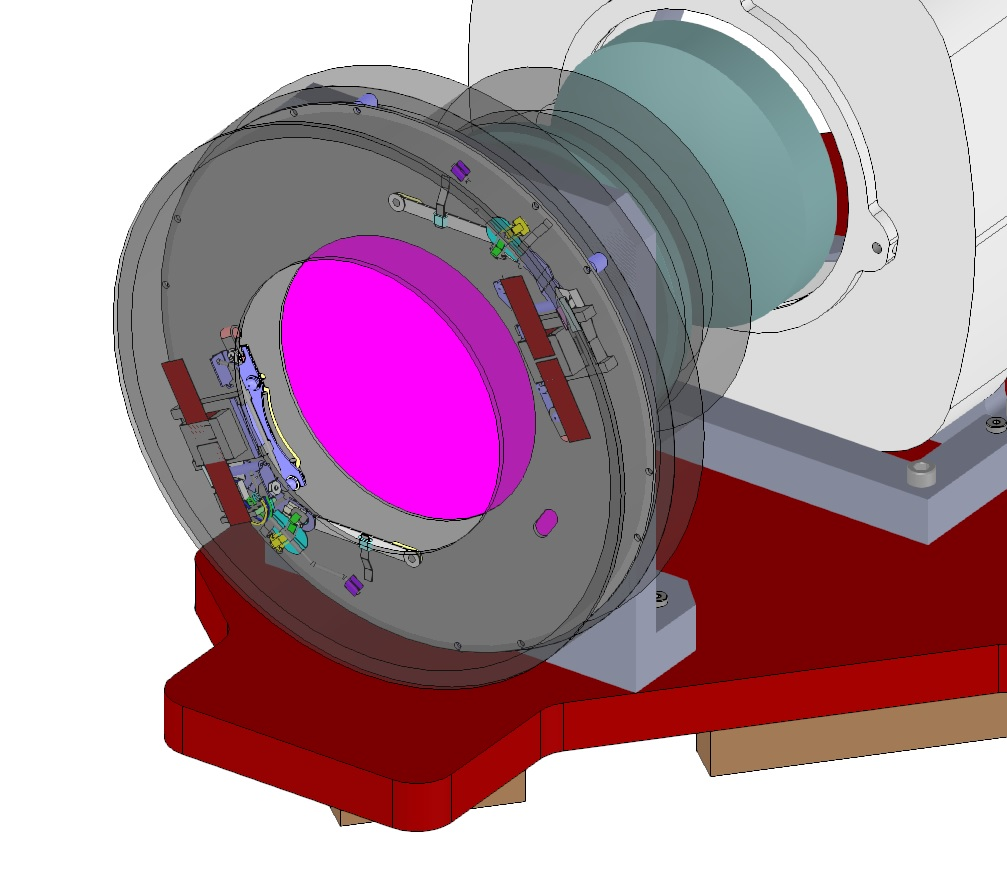
\includegraphics[width=\linewidth]{figures/alex-S1.jpg}
%\end{center}
%\caption{The Shutter on the CAGIRE WOB.}
%\label{figure:alex-S1}
%\end{figure}

\clearpage
\section{Mechanism MTBF}

\subsection{Shutters}

Vincent Associates have informed us that the CS90 shutters we are using with both of the DDRAGO CCDs and in the CAGIRE warm optics have a mean lifetime of approximately half a million cycles.

For DDRAGO, we anticipate that the shutters will be used once per minute (60 second exposures) for 12 hours per night for 80\% of nights. Thus, the MTBF will be about 2.4 years. We will provide a spare and document the replacement process.

%Since we have two CCDs, we expect about one shutter failure per year. Thus, provision of spares and the process of replacing shutters is vitally important.

%For CAGIRE, the MTBF will depend on the mode in which the shutter are used. If it is used at the end of each exposure, we anticipate that it will be used twice per minute (30 second exposures) for 12 hours per night for 80\% of nights. Thus, the MTBF will be about 1.2 years. If it is only used during the day and during slews, we anticipate that the life will be at least 10 times longer (one slew every five minutes).

%In both cases, we need to decide if we should replace the shutters proactively before they fail. However, since the shutters cost about US\$6000 each, the additional cost of this would not be trivial. This is something that needs to be discussed with the GFT project and the OAN.

\subsection{Filter Wheels}

We do not have lifetimes for the FLI filter wheels we are using in DDRAGO.

Nevertheless, we have operated a similar wheel in the C0 channel of RATIR for five years without any failures. This suggests that FLI filter wheels are reliable.

We will procure a total of three wheels, two for service and one spare. If one fails, we will replace it with the spare and send it to FLI for repair.

%\subsection{Focuser}

%Again, we do not have lifetimes for the FLI Atlas focuser we are using in the CAGIRE warm optics.

%Nevertheless, we have operated four similar focusers in RATIR (two PDF models for the science CCDs and two DF-2 models for the finders) for five years without any failure. This suggests that these are reliable.

%We will procure a spare focuser. If the focuser fails, we will replace it with the spare and send it to FLI for repair.

\clearpage
\section{Environmental Sensors}

\begin{figure}
\begin{center}
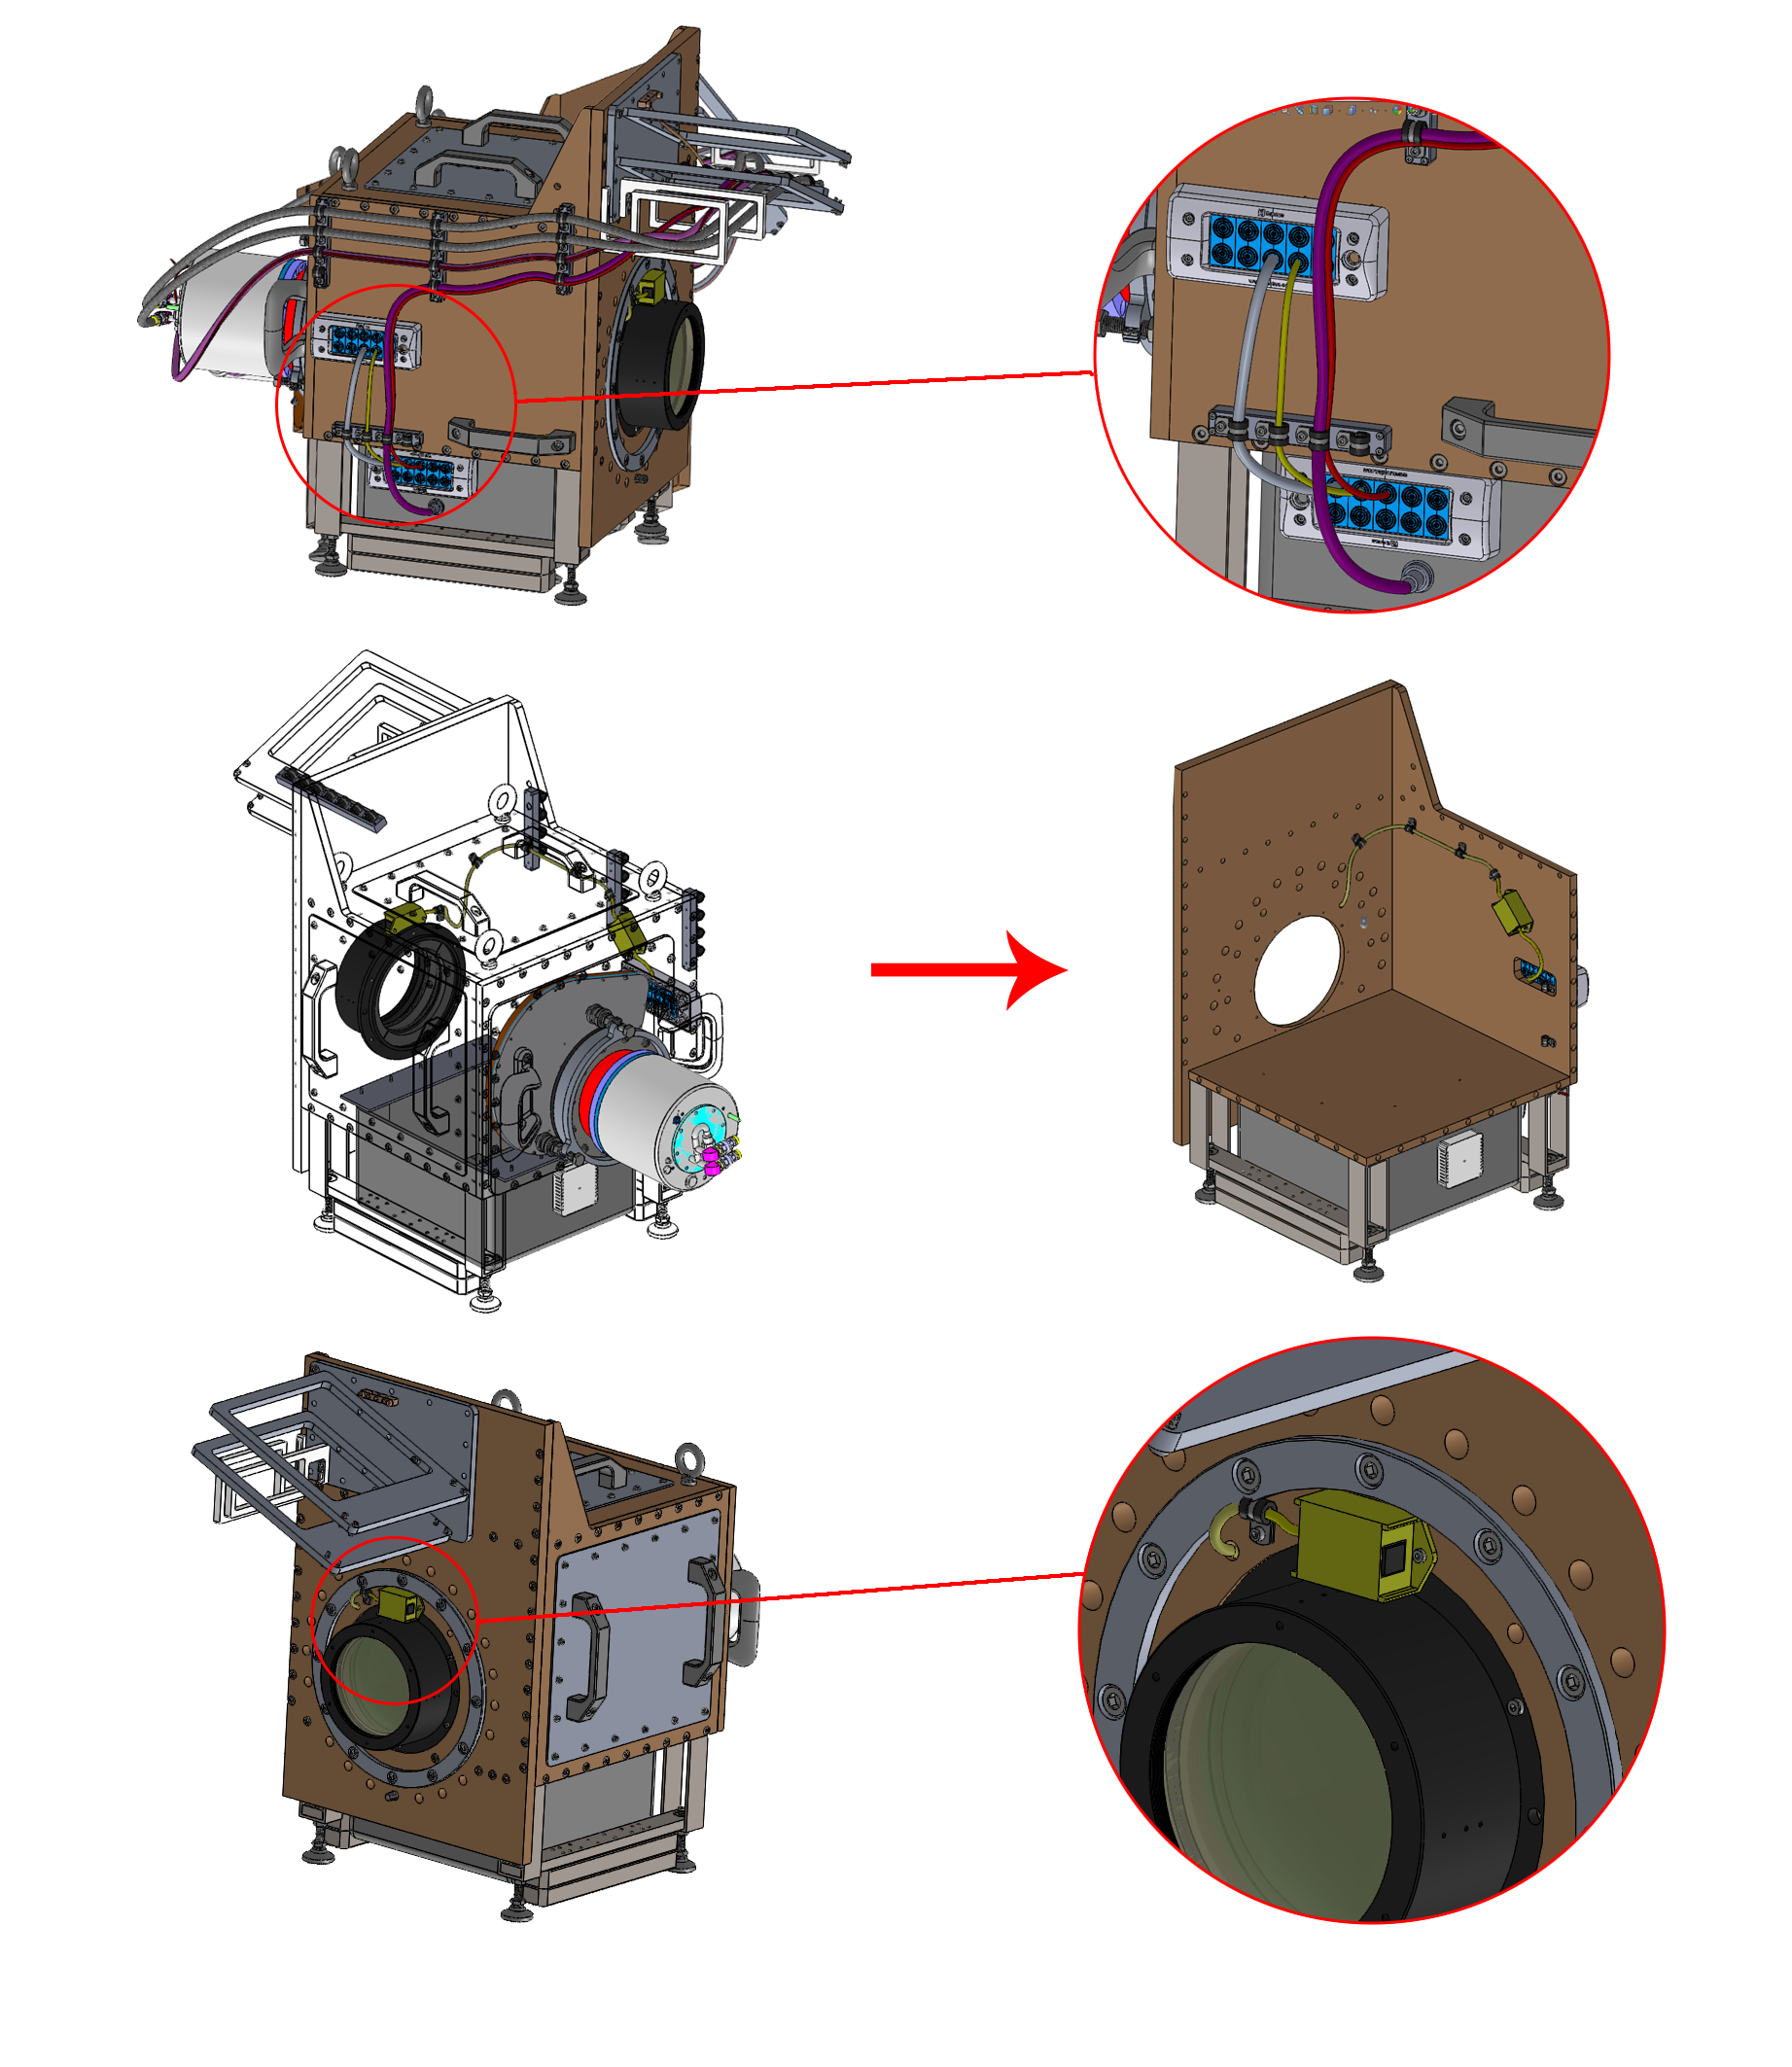
\includegraphics[width=\linewidth]{newfigures/Fig8_1.png}
\end{center}
\caption{The Environmental Sensors in the Support Structure for DDRAGO.}
\label{figure:alex-environmental-sensors}
\end{figure}

Figure~\ref{figure:alex-environmental-sensors} shows the environmental sensors installed on the support structure. These is one MS-TH 1-wire temperature and humidity sensor in the support structure and one MS-TH in the derotator tunnel adjacent to OML1L2.

The MS-TH sensors are wired in series from an adapter in the DDRAGO close electronics cabinet. The cable enters the support structure through the RoxTec CM 20w40 cable seal mounted on plat FP4 and leaves through a hole in the flange of plate FP1. The hole will be filled with silicone once the cable has been installed.

%Also, at the request of the CAGIRE team, we include an EDS OW-ENV-THPL sensor for their use.  The cable for this enters through the SS-CAP2 cable-access plate

\clearpage
\section{Detector Orientation}

\begin{figure}[bp]
\begin{center}
\includegraphics[width=\linewidth]{newfigures/CCD-Orientation.png}
\end{center}
\caption{The rotation of the CCD by 13 degrees with respect to the support structure.}
\label{figure:ccd-rotation}
\end{figure}

The orientation of the filter wheel and hence the square filters is fixed by our desire to use the same removable plate RP3 in the interim instrument and in the blue channel of the definitive instrument. In the definitive instrument, avoiding interference with the derotator forces us to choose a specific orientation that is rotated with respect to the instrument support structure. In the interim instrument, we could have avoided this by making the support structure larger, but did not see a compelling reason to do so.

To avoid vignetting, the CCD must be aligned with the square filters and so in turn is also rotated with respect to the support structure of the instrument.

When the instrument is shown at the nominal center of the $\pm60$ degree range of the derotator, the plates FP3 and FP5 are horizontal, with FP3 at the top, the plates FP2 and FP4 are vertical, and the CCD is rotated by 13 degrees clockwise when looking along the axis of the derotator from outside. This is shown in Figure~\ref{figure:ccd-rotation}.

\clearpage
\section{Cables and Hoses}

The cables and hoses which reach the instrument from the cable wrap are: two coolant hoses; one power cable for the CCD; one control fiber for the CCD; one power cable for the close electronics; one control fiber pair for the close electronics; and ground cable.

The cable wrap (supplied with the telescope) is supported by the cable wrap support (DR-ME-IN-CWS). 

The ground cable is connected to a ground connector (McMaster model 2450k1) on the cable wrap support. 

The other cables and hoses are then guided onto the plate FP4 by the cable support guides (DR-ME-IN-CSG1/2) in a way that does not require any cable or hose to be bent more sharply than the minimum bending radius. The cables and hoses are then supported by FP4 to their final destination, either the close electronics (CE) or the detector (BDET). We use neoprene-lined loop clamps (McMaster model 3177T120) to support the cables and hoses. Those at the mouth of the cable wrap are constrained to not rotate, so that they support the hoses axially. The other clamps can rotate slightly. The fibers will follow their corresponding power cables and will not pass through the clamps but rather around them.

\begin{figure}
\begin{center}
\includegraphics[width=\linewidth]{newfigures/Fig9_1.png}
\end{center}
\caption{The cable and hose management.}
\label{figure:alex-cables-and-hoses}
\end{figure}

Three cables (one for the environmental sensores, one for filter wheel power, and one for filter wheel control) leave the close electronics cabinet (DR-CO-CE) and enter the support structure through Roxtec CM 20w40 cable seals. Each cable seal is capable of passing 10 cables from 3.5 to 16.5 mm in diameter.

\begin{figure}
\begin{center}
\includegraphics[width=\linewidth]{newfigures/FigDero.png}
\end{center}
\caption[The cable guides.]{The cable guides allow the derotator to move through its $\pm60$ degree range without any interference with the cables.}
\label{figure:cable-rotation}
\end{figure}

Figure~\ref{figure:cable-rotation} shows that the cable guides allow the derotator to move through its $\pm60$ degree range about its nominal position without any interference with the cables. However, if the derotator rotates outside this range, there is a possible interference between the cables and the derotator motor and drive. We need to clarify with the telescope vendor if this is a possibility, and if so install a hard stop to prevent it.

\clearpage
\section{Covers}

\begin{figure}[p]
\begin{center}
\includegraphics[width=0.7\linewidth]{figures/DR-ME-OML1L2-FC-EXV.PDF}
\end{center}
\caption{The DR-ME-OML1L2-FC front cover mounted on DR-ME-OML1L2-BAR.}
\label{figure:oml1l2-fc}
\end{figure}

\begin{figure}[p]
\begin{center}
\includegraphics[width=0.7\linewidth]{figures/DR-ME-OML3-FC-EXV.PDF}
\end{center}
\caption{The DR-ME-OML3-FC front cover mounted on DR-ME-OML3-BAR.}
\label{figure:oml3-fc}
\end{figure}

\begin{figure}[p]
\begin{center}
\includegraphics[width=\linewidth]{newfigures/SSCoverPlates.png}
\end{center}
\caption{The DR-ME-OML1L2-RC, DR-ME-OML3-RC, and DR-ME-IN-FSSC cover.}
\label{figure:covers}
\end{figure}

We will manufacture front and rear covers for OML1L2 and OML3 to protect the lenses and a cover to substitute OMBDET during transport, storage, and maintenance. These will be manufactured from Nylamid. The front covers attach to the corresponding barrels and the rear covers to the support structure (for OML1L2) or to the L-bracket (OML3). The covers are shown in Figures~\ref{figure:oml1l2-fc}, \ref{figure:oml3-fc}, and \ref{figure:covers}.

\clearpage
\section{Mass and Torques}

\subsection{Mass Budget}

%\TODO{Add cables and hoses to mass budget. Make more precise estimates for the electronics and fixing hardware.}

Table~\ref{table:mass} shows our current mass budget for the DDRAGO interim instrument of 112~kg.

\begin{table}[p]
\caption{Mass Budget}
\label{table:mass}
\begin{center}
\begin{tabular}{llcl}
\hline
Component&Code&Mass&Source\\
&(kg)&\\
\hline
Support Structure                      &IN       &\phantom{0}60.82&Model\\
Lenses                                 &L1/L2/L3 &\phantom{00}3.24&Model\\
Optomechanics for L1/L2                &OML1L2   &\phantom{00}1.40&Model\\
Optomechanics for L3                   &OML3     &\phantom{00}1.01&Model\\
Optomechanics for CCD and filter wheel &OMBDET   &\phantom{00}1.33&Model\\
CCD                                    &BDET     &\phantom{0}11.40&Manufacturer\\
Filter wheel                           &BFW      &\phantom{00}2.04&Measured\\
Filters                                &FL       &\phantom{00}0.32&Model\\
Electronics cabinet                    &CE       &\phantom{00}5.00&Estimated\\
Electronics cabinet interface          &         &\phantom{00}1.00&Estimated\\
Hoses and cables                       &         &\phantom{00}1.21&Model\\
Counterweights                         &         &\phantom{0}14.66&Model\\
Mechanical hardware                    &         &\phantom{00}8.00&Estimated\\
\hline
Total                                  &         &\phantom{}111.44\\
%DDRAGO\\
%Support Structure             &\phantom{0}94.56\phantom{}&Model\\
%Optics                        &\phantom{00}4.50\phantom{}&Model\\
%L1+L2 Barrel                  &\phantom{00}2.60\phantom{}&Model\\
%D1, D2 and CP supports        &\phantom{00}3.63\phantom{}&Model\\
%L3 Barrel/Interface           &\phantom{00}1.13\phantom{}&Model\\
%L4 Barrel/Interface           &\phantom{00}1.13\phantom{}&Model\\
%Blue CCD Interface            &\phantom{00}1.08\phantom{}&Model\\
%Blue CCD                      &\phantom{0}11.40\phantom{}&Manufacturer\\
%Blue FW                       &\phantom{00}1.50\phantom{}&Manufacturer\\
%Red CCD interface             &\phantom{00}1.08\phantom{}&Model\\
%Red CCD                       &\phantom{0}11.40\phantom{}&Manufacturer\\
%Red FW                        &\phantom{00}1.50\phantom{}&Manufacturer\\
%Electronics Cabinet           &\phantom{00}5\phantom{.00}&Estimate\\
%Electronics Cabinet	Interface &\phantom{00}1\phantom{.00}&Estimate\\
%Fixing Hardware               &\phantom{00}6\phantom{.00}&Estimate\\
%SUBTOTAL for DDRAGO           &\phantom{}146.54\phantom{}\\
%\hline
%CAGIRE\\
%WOB Optics                    &\phantom{00}4\phantom{.00}&Model\\
%Lens Barrels/Interfaces       &\phantom{00}3.85\phantom{}&Estimate\\
%FM Supports                   &\phantom{00}4.45\phantom{}&Estimate\\
%Mask Supports                 &\phantom{00}1.4\phantom{0}&Estimate\\
%Shutter                       &\phantom{00}1\phantom{.00}&Estimate\\
%Focuser                       &\phantom{00}1.5\phantom{0}&Manufacturer\\
%Focuser Interface             &\phantom{00}0.57\phantom{}&Estimate\\
%WOB Plate                     &\phantom{00}4.29\phantom{}&Model\\
%Cryostat                      &\phantom{0}50\phantom{.00}&Estimate\\
%Electronics Cabinet           &\phantom{0}30\phantom{.00}&Estimate\\
%Electronics Cabinet Interface &\phantom{00}4\phantom{.00}&Estimate\\
%Fixing Hardware               &\phantom{00}6\phantom{.00}&Estimate\\
%SUBTOTAL for CAGIRE           &\phantom{}111.06\phantom{}\\
%\hline
%TOTAL for DDRAGO and CAGIRE   &\phantom{}258.60\\
\hline
\end{tabular}
\end{center}
\end{table}


\subsection{Center of Mass}

\begin{figure}[p]
\begin{center}
\includegraphics[width=\linewidth]{newfigures/CoMIN.png}
\end{center}
\caption[The Center of Mass.]{The center of mass without counter-weights (above) and with counterweights (below)}
\label{figure:alex-com}
\end{figure}

The center of mass without counterweights is at $x = -4$ cm, $y = -1$ cm, and $z = 24$~cm (relative to an origin at the center of the derotator). 
Figure~\ref{figure:alex-com} shows that the coordinates of the center of mass  with counterweights is at $x = -2$ cm, $y = 0$~cm, and $z = 24$~cm.

%We estimate that putting approximately 42~kg on CWE3A-CWE3B (below the blue detector) and 14~kg on CWE3C-CWE3D (next to the CAGIRE cryostat interface) will move the center of mass to the axis of the derotator. Each CWE pair can easily accommodate 60~kg. The precise weight and distribution of the counter-weights will be determined iteratively when the instrument is mounted on the telescope.

\subsection{Torque on Derotator Motor}

The mass density of cables in the cable wrap is about 0.713 \unit{kg\,m^{-1}}. The linear mass density of the cable chain itself is 3.05~\unit{kg\,m^{-1}}. The length is about 1.7 meters and the cable wrap is attached at a radius of about 0.31~m. Thus, the torque of the cable wrap alone on the derotator is about 19.4~\unit{N\,m}.

The torque of the DDRAGO interim imager is about 24.0~\unit{N\,m}.

The combined torque of both is about 35~\unit{N\,m}. This is well within the 100~\unit{N\,m} limit on the derotator motor.

%We will balance the instrument using counter-weights attached to the counter-weight extensions CWE3A--CWE3D. These operate in pairs and masses are placed between them and fastened at both ends. Initial calculations suggest that for the DDRAGO and CAGIRE together we will need to add about 100~kg of mass (see Figure~\ref{figure:alex-com-balanced}). This is certainly possible.

%We may be able to reduce the mass of counter-weights by perhaps a factor of two by moving the CAGIRE electronics to a more optimal position.

\subsection{Torque on Derotator Flange}

The torque on the derotator flange for the DDRAGO interim instrument with counter-weights is about 285~\unit{N\,m}. This is well below the maximum permitted torque of 1,715~\unit{N\,m}.

\clearpage
\section{Surface Finishes}

Requirement GFT-REQ-47 in the FPRD requires us to ensure that all mechanical surfaces that are exposed to the beam have a reflectivity of less than 8\%.

For external parts and surfaces, we will use a standard black anodization. 

For most internal parts and surfaces, we will use sandblasting, anodization, and Krylon 1602 Ultra-Flat Black paint. This is a hardened carbon-black paint with a reflectivity of less than 4\% from the optical to the infrared. We used this finish in the RATIR cryostat, and witness tests at GSFC showed reflectivities of 3.25\% to 3.75\% from 600 to 2500 nm after painting. (We have no quantitative data below 600 nm, but since the paint visually has no color cast, we have qualitative evidence that the reflectivity is uniformly low from 400 to 700 nm.) We have applied this finish to witness samples of aluminum to confirm its robustness. (The RATIR cryostat was manufactured at GSFC.) We discovered that sandblasting seems to give better adherence than using a self-etching primer. Anodization gives additional protection.

Reference surfaces between aluminum parts require some care. For the optomechanical mounts, we will typically finish all surfaces except reference surfaces and threads, sand blast and anodize, finish the reference surfaces and manufacture the threads. Then, after assembly and verification, we will paint the unpainted regions around the reference surfaces. For the support structure, we will paint the inner surfaces after assembly, mounting all of the optomechanical mounts, and verification.

Despite this, we note that we cannot paint some reference surfaces, non-aluminium materials, or screw threads. A full list of unpainted internal surfaces is:

\begin{itemize}
\item
The reference surfaces between aluminum and glass in OML1L2-BAR, OML1L2-SPA, and OML3-BAR. However, we have shown that the reflections are shaded or benign (\ref{optics}).
\item
The inside surfaces of the teflon friction reducing rings OML1L2-FRR and OML3-FRR. We will make these inner diameter of these slightly larger than necessary so that they are shielded by the corresponding O-ring holder (OML1L2-ORH and OML3-ORH).
\item
The screw threads for the preload rings in the lens barrels OML1L2-BAR, OML1L2-SPA, and OML3-BAR. These will be shaded by the corresponding preload rings OML1L2-PLR, OML1L2-PLR, OML3-PLR.
%\item
%The FPM cushions in the optomechanical mounts OMD1, OMD2, and OMCP. Here our only mitgation is using black material, but we have no information on the actual reflectivity. We note, however, that the cushions are outside the nominal beam.
\end{itemize}

%\clearpage
%\section{Support Trolley}
%
%\TODO{Design the trolley}
%
%We will provide a support trolley capable of supporting DDRAGO/CAGIRE in the laboratory, at the OHP, and at the OAN. 
%
%The support trolley will consist of three parts: an upper part that mates to the instrument, a lower part with wheels, and a middle spacer part that adjusts the the desired height.
%
%The upper part of the trolley will be common to both configurations. It will fasten to the counter-weight extensions CW3A--CW3D on the fixed plate FP3 of the support structure in a manner TBD. It will, to the extent necessary, allow for the removal of the electronics boxes, cryostat, CCDs, and structure walls. It will firmly fasten to the support structure using bolts so that it will be stable even if some of these components are removed.
%
%The lower part of the trolley will have wheels or castors in order to move horizontally in two dimensions on a relatively flat surface. It will also have height adjustment of perhaps $\pm1$~cm. It will have a wide wheel base so that it will be stable even if components are removed from the instrument.
%
%There will be two middle sections, one for OHP and one for the OAN. The detailed design of these will depend on the height between the derotator axis and the floor, which is still TBD.
%
%%In the “short” configuration, the upper part of the trolley will mate to a lower part that will hold the instruments perhaps 20 cm above the floor. The short configuration will be used in the laboratory and at the OHP. At the OHP, we propose to mount and dismount the instrument by installing the lower part of the trolley on a (rented) scissor lift. If necessary, we will install a temporary wooden floor on the scissor lift to facilitate moving the trolley horizontally.
%
%%In the “tall” configuration, the upper part of the trolley will mate to a lower part that will hold the instrument at approximately the correct height for mounting or dismounting the instrument at the OAN.
%
%% NOT FALL OVER EVEN IF WE REMOVE THE CRYOSTAT
%%










\end{document}
